% Created 2014-06-27 Fri 20:54
\documentclass[11pt]{report}
\usepackage[utf8]{inputenc}
\usepackage[T1]{fontenc}
\usepackage{fixltx2e}
\usepackage{graphicx}
\usepackage{longtable}
\usepackage{float}
\usepackage{wrapfig}
\usepackage{soul}
\usepackage{textcomp}
\usepackage{marvosym}
\usepackage{wasysym}
\usepackage{latexsym}
\usepackage{amssymb}
\usepackage{hyperref}
\tolerance=1000
\usepackage{german}
\providecommand{\alert}[1]{\textbf{#1}}

\title{Das RubyFrontier-Buch\\Statische Seiten mit allem Komfort}
\author{Jörg Kantel}
\date{\today}
\hypersetup{
  pdfkeywords={},
  pdfsubject={},
  pdfcreator={Emacs Org-mode version 7.9.3f}}

\begin{document}

\maketitle

\setcounter{tocdepth}{4}
\tableofcontents
\vspace*{1cm}

\part{Übersicht und Installation}
\label{sec-1}
\chapter{Einleitung}
\label{sec-1-1}
\section{Was ist RubyFrontier?}
\label{sec-1-1-1}

    
\subsection{Die Kurzfassung}
\label{sec-1-1-1-1}


RubyFrontier ist ein Werkzeug, um statische Webseiten in einem
Texteditor unter MacOS X) zu erstellen (zur Zeit wird leider nur der
(kommerzielle) Editor TextMate unterstützt). Die Software wurde von
Matt Neuburg in der Programmiersprache Ruby geschrieben und kann mit
Ruby-Skripten erweitert werden.
\subsection{Die Langfassung (und ein wenig Computer- und Netzgeschichte)}
\label{sec-1-1-1-2}


Vor langer, langer Zeit, als es das Internet noch gar nicht wirklich
gab, gab es für die Macintosh-Computer eine Software, die Frontier
hieß. Sie war — bis zur Version 5.0.1 — frei (im Sinne von Freibier)
und so etwas wie eine eierlegende Wollmilchsau. Sie konnte andere
Apple-Programme steuern (lange bevor es AppleScript gab), sie konnte
Daten in einer integrierten Objekt-Datenbank (Look ma, no SQL)
speichern, sie war ein Outliner und ab der Version 5 auch ein
Webserver auf dem Desktop. Vor allem aber besaß sie seit der Version
4.2.3 ein sogenanntes Website Framework, mit dem man für die damaligen
Verhältnisse einfach und effektiv statische Webseiten herausschrieben
konnte. Und sie besaß eine integrierte Skriptsprache, UserTalk, mit
der man das System an seine Bedürfnisse anpassen und experimentieren
konnte. Frontier war 1988 von Dave Winer, einem Weblog-Pionier
entwickelt worden und wurde von seiner Firma UserLand vertrieben, die
Versionen größer 5.0.1 waren kommerziell und mußten bezahlt werden.

\begin{figure}[h!]
\centering
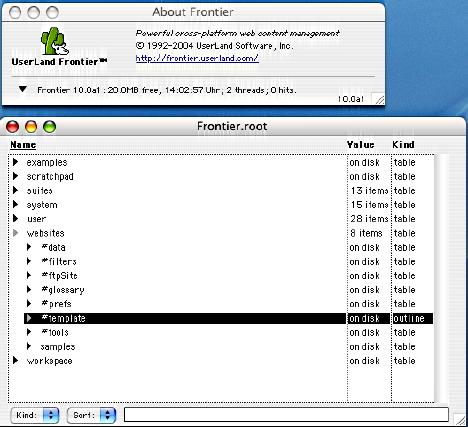
\includegraphics[width=0.7\textwidth]{./images/frontierdesktop.jpg}
\caption{\label{frontierdesktop}Frontier-Desktop}
\end{figure}

Winer hatte und hat bis heute immer großartige Ideen, leider haperte
es häufig an der Ausführung. So ignoriert er bis heute — obwohl er ein
Großneffe Arno Schmidts ist —, daß es auch andere Sprachen als
Englisch gibt und diese womöglich einer besonderen Beachtung wegen
ihrer Schriftzeichen (zum Beispiel Umlaute) benötigen. Ich hatte meine
ersten Schritte im Web mit Frontier begonnen und auch mein Weblog, der
Schockwellenreiter lief in de ersten Jahren mit dem auf Frontier
basierenden Content Management System (CMS) Manila auf einem von
Winers Servern. Später wechselte ich dann zu dem ebenfalls auf
Frontier basierenden Radio UserLand, einem CMS und Weblog-Tool, das
als Webserver auf dem Desktop arbeitete und statische Seiten auf den
Server meiner Wahl herausrenderte.

\begin{figure}[h!]
\centering
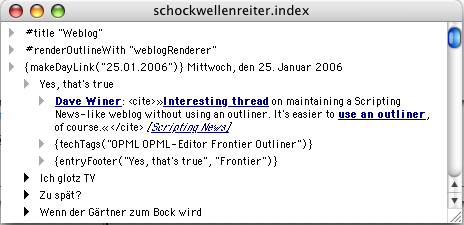
\includegraphics[width=0.7\textwidth]{./images/outliningswr.png}
\caption{\label{outliner}Outliner}
\end{figure}

Frontier und Radio UserLand waren über Jahre so etwas wie mein Uber
Tool, ich programmierte fast alle meine Web-Aktivitäten damit, zum
Beispiel auch das Virtual Laboratory for Physiology, eine Website zur
Erforschung der Medizingeschichte des 19. Jahrhunderts (aber auch hier
wechselte ich vor einigen Jahren zu Zope — siehe unten).


Als Frontier dann kommerziell und die Objekt Datenbank (ODB) ob ihrer
Größe instabil wurde, wechselte ich zu Zope, einem auf der
Programmiersprache Python basierendem CMS, das große Ähnlichkeiten mit
Frontier hatte. Doch einige Jahre später — Dave Winer hatte sich aus
gesundheitlichen Gründen von UserLand zurückgezogen — wurde Frontier
Open Source und ich stieg sofort wieder um und nutzte von 2005 bis
2009 das Static Site Framework um mein Blog zu erstellen. Leider gab
es nicht genug Entwickler, um das Open Source Frontier nicht nur am
Leben zu erhalten, sondern weiterzuentwickeln und die Fork, die Winer
mit seinem OPML Editor (ein nahzu komplettes Frontier) anbot, hatte
alles, nur nicht das Static Site Framework (auf meine Veranlassung war
es kurzfristig unter den Tools dabei, verschwand dann aber aus mir
unbekannten Gründen wieder aus dem Angebot).


Aber zuerst einmal war ich begeistert und schrieb auch ein Tutorial
über Frontiers Static Site Framework, das ich für diese Einführung in
RubyFrontier überarbeitet habe.


So läuft mein Blog seitdem mit WordPress, ich bin aber nicht wirklich
glücklich darüber und denke immer wieder mal nach, ob ich nicht wieder
ein statisches Blog schreibe — evtl. tatsächlich mit
RubyFrontier. (Eigentlich habe ich schon alles dafür konzipiert, nur
es muß etliches programmiert werden — speziell das Herausschreiben des
RSS-Feeds — und ich bin bisher einfach noch nicht dazu gekommen. Aber
wenn dieses Buch fertig geschrieben ist, habe ich vielleicht wieder
ein wenig mehr Zeit.)


Wie dem auch sei, Winers Version von Frontier, der OPML Editor, lebt
und wird auch weiterentwickelt. Aber ihm fehlt einiges, speziell die
Möglichkeit, statische Seiten herauszuschreiben. Und in diese Bresche
sprang Matt Neuburg, einst ebenfalls ein großer Frontier-Fan, der auch
ein Buch darüber veröffentlicht hatte (das über Jahre so etwas wie
meine Bibel war), mit RubyFrontier.
\section{Warum RubyFrontier?}
\label{sec-1-1-2}
\subsection{Warum überhaupt statische Seiten?}
\label{sec-1-1-2-1}


\begin{figure}[h!]
\centering
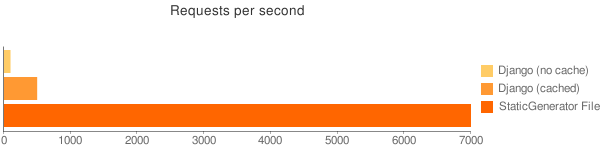
\includegraphics[width=0.7\textwidth]{./images/staticgenerator-chart.png}
\caption{\label{staticpages}Statische Seiten sind schnell}
\end{figure}

Statische Seiten sind unheimlich schnell. Obiger Vergleich zeigt, daß
statische Seiten bis zu 14 mal schneller als (selbst gecachte)
dynamisch erzeugte Seiten vom Browser geladen werden.


Statische Seiten sind sicher: Es gibt für Angreifer keine Möglichkeit,
mit irgendwelchen Skripten ihren Webauftritt zu manipulieren. Denn in
der Regel liegen die Quellen auf Ihrem Desktop. Und da muß ein
Angreifer erst einmal herankommen. Okay, wenn Sie Ihren Laptop mit all
Ihren Quellen im Zug liegen lassen — wie es angeblich einigen
britischen Geheimdienstlern passiert sein soll —, dann haben auch Sie
mit Zitronen gehandelt, aber unter normalen Umständen sind Sie der
einzige, der die Integrität Ihrer Quellen beschädigen kann. Das
natürlich eine vernünftige Backup-Strategie die Sicherheit fördert,
muß ich Ihnen sicher nicht erst erzählen, oder?


Statische Seiten gehören Ihnen: Wenn Sie RubyFrontier (aber auch
andere Template Toolkits wie das schon erwähnte Perl Template Toolkit
oder Ninja2) nutzen, rendert die Software die Seiten auf Ihrem Rechner
heraus. Und auch die Quelltexte liegen auf Ihrem Rechner. Falls also
irgendein Provider beschließt, Sie zu zensieren oder auch aus
finanziellen Gründen den Laden schließen zu wollen, suchen Sie sich
einfach einen anderen und laden die Seiten da wieder hoch.


Natürlich funktioniert ein Framework wie RubyFrontier zur Erstellung
statischer Seiten nicht wie ein Webserver auf dem Desktop. Dabei hat
diese Idee durchaus Charme und es gibt einige Anwendungen, die die
Nützlichkeit dieses Konzeptes zeigen, zum Beispiel die
Mathematik-Software Sage. Ich habe sie auch nicht völlig aus den Augen
verloren, setze da aber weniger auf den OPML Editor (obwohl auch das
durchaus Charme hätte), sondern auf den einfach zu installierenden in
Python geschriebenen Webserver web2py. Vermutlich wird eine Einführung
in dieses Framewokr mein nächstes Buchprojekt.
\subsection{RubyFrontier}
\label{sec-1-1-2-2}


Es gibt viele Tools, um statische Seiten zu erzeugen. Die meisten sind
Template Engines, die sowohl statische Seiten erzeugen, aber auch im
Hintergrund für ein dynamisches Web Framework agieren können. Mein
Favorit war lange Zeit das in der Skriptsprache Perl geschriebene Perl
Template Toolkit, aber auch andere wie Jekyll (Ruby) oder Ninja2
(Python) hatten meine Sympathie. Bis mir dann auffiel, daß alle diese
Werkzeuge einen »Profi«-Ansatz hatten, das heißt, daß es keinen
einfachen Einstieg für Menschen gab, die nicht unbedingt auf ein
abgeschlossenes Informatik-Studium zurückblicken konnten. Und das,
obwohl fast alle das Gegenteil behaupteten. RubyFrontier wiederum ist
nach Einschätzung seines Schöpfers zwar ein Werkzeug für
Programmierer, doch wie ich Ihnen in den nächsten Abschnitten zeigen
werde, ist der Einstieg auch für Nicht-Programmierer doch recht
einfach.


Ein wenig skripten muß man zwar auch hier und wenn man Ruby gut
beherrscht, kann man sich nahezu alle Wünsche, die man an eine
Template-Engine hat, mit RubyFrontier erfüllen. Aber der Einstieg ist
— dank der hervorragenden Integration in TextMate — einfach und leicht
nachvollziehbar.
\subsection{RubyFrontiers Grenzen}
\label{sec-1-1-2-3}


RubyFrontier ist sehr schnell — bedeutend schneller als es Frontier je
war —, aber es gibt Situationen, bei denen der Einsatz nicht mehr
sinnvoll ist. Falls Sie zum Beispiel zehntausende von Katalog-Seiten
herausschreiben müssen, dann sollten Sie auf andere Werkzeuge
zurückgreifen. Der Glossary-Mechanismus von RubyFrontier ist sinnvoll
und erleichtert Ihnen die Arbeit ungemein, aber er kostet auch Zeit,
und zwar viel Zeit. Und bei zehntausenden von Einträgen kann das
Herausschreiben der HTML-Seiten auch schon mal einen Tag und eine
Nacht oder noch länger dauern. Glauben Sie mir, ich habe es mit einem
Katalog des Nachlasses eines vor etwa 100 Jahren gestorbenen
Wissenschaftlers probiert (circa 80.000 HTML-Seiten) und mir dann
entnervt ein kleines, schmutziges Skript in Python geschrieben. Das
konnte zwar nur die Webseiten des Katalogs mit den dazugehörigen Scans
rausschreiben und sonst gar nichts, war aber dafür nach wenigen
Minuten damit fertig. RubyFrontier benötigte für die gleiche Aufgabe
etwa 36 Stunden.


Aber für einen durschnittlichen Web-Auftritt selbst mit ein paar
hundert Seiten ist RubyFrontier durchaus das geeignete Werkzeug.
\subsection{Mac only}
\label{sec-1-1-2-4}


Bis dato läuft RubyFrontier nur auf Apple-Rechnern unter MacOS X und
auch nur mit TextMate. Das ist nicht zwingend, denn Ruby läuft
eigentlich auf so ziemlich allem, was die Bezeichnung Betriebssystem
verdient (also auch unter Windows und den diversen
Linux-/Unix-Derivaten). Gelegentlich hat Matt verlauten lassen, daß er
daran denke, diese Abhängigkeiten zu beseitigen, aber es scheint nicht
wirklich eine hohe Priorität zu haben. Mein Favorit wäre ja der in
Java geschriebene, plattformübergreifende Editor jEdit, für den es ein
komfortables Project Viewer-Plugin gibt, mit dem ich alle meine Perl
Template Toolkit-Projekte verwalte.

\begin{figure}[h!]
\centering
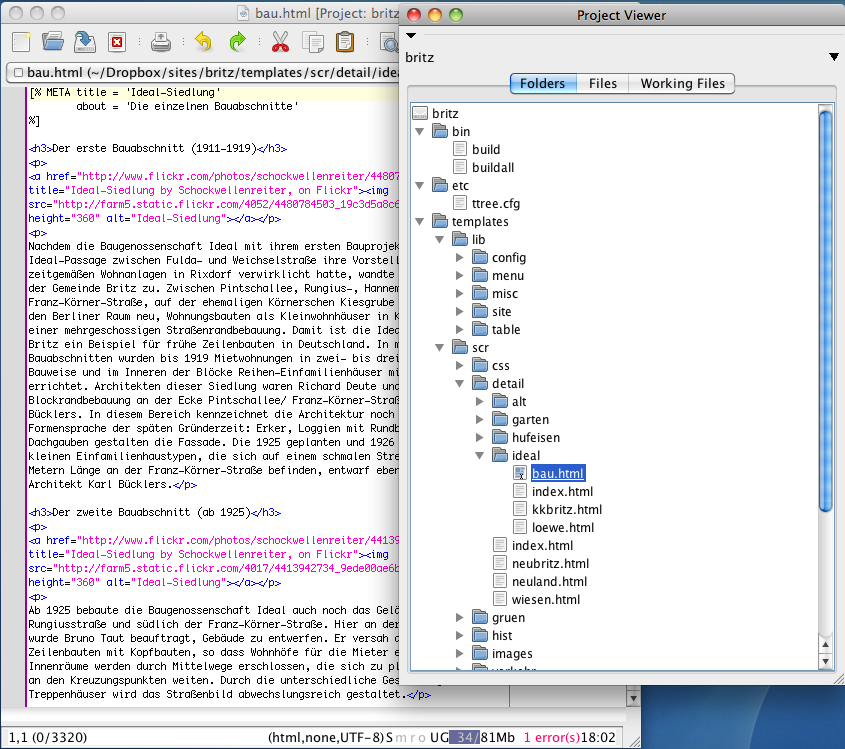
\includegraphics[width=0.7\textwidth]{./images/projektviewer-in-jedit.png}
\caption{\label{jeditsidedrawer}Side Drawer in jEdit}
\end{figure}

Aber vielleicht setzt sich auch mal jemand anders daran und baut
RubyFrontier plattformübergreifend aus. RubyFrontier ist schließlich
Open Source und steht unter der äußerst liberalen MIT-Lizenz. Und es
sind ganze elf Befehle, die anzupassen und mit dem Text-Editor zu
verheiraten sind. Dem Absatz dieses Buches würde es jedenfalls
bestimmt nicht schaden, wenn RubyFrontier auch unter Windows und Linux
laufen würde.
\subsection{Kein Outliner}
\label{sec-1-1-2-5}


Einer der großen Stärken von Frontier war (und ist es beim OPML Editor
noch heute), daß es mit Outlines, also strukturierten, eingerückten
und ausklappbaren Texten umgehen und diese auch skripten konnte. Mein
Weblogzum Beispiel war so organisiert, daß in der ersten Ebene die
Überschriften eines Beitrags standen und in der zweiten Ebene und
darunter der eigentliche Text. Und der Outline-Renderer (ein
UserTalk-Skript) nutzte diese Struktur um dann nicht nur das
eigentliche Weblog herauszuschreiben, sondern auch um den RSS-Feed zu
produzieren.


Matt Neuburg hat zwar die wichtigsten Outline-Kommandos aus Frontier
nach RubyFrontier portiert, aber TextMate ist nun mal kein
Outliner. Wer Outlines benötigt, muß diese mit einem externen Programm
im OPML-Format erzeugen (dazu böte sich unter anderem natürlich Dave
Winers OPML Editor als Open Source-Programm an, aber auch das
kommerzielle OmniOutliner ab ca. 40 US-\$ kann OPML-Dateien
herausschreiben).


\begin{figure}[h!]
\centering
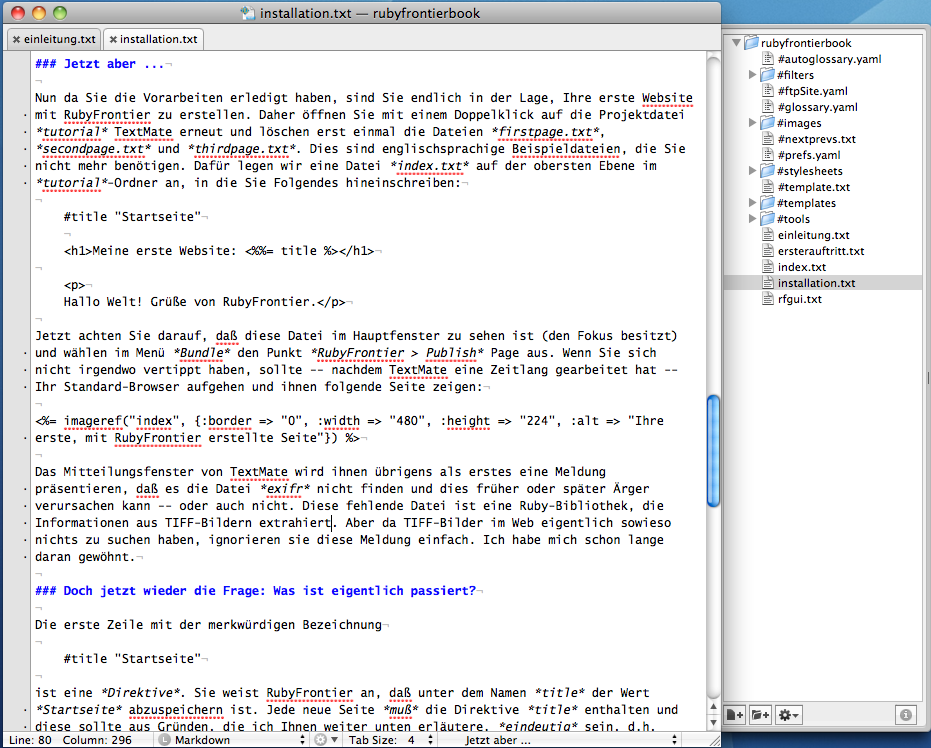
\includegraphics[width=0.7\textwidth]{./images/markdown-in-rubyfrontier.png}
\caption{\label{markdownrf}Markdown in RubyFrontier}
\end{figure}

Aber es gibt auch eine interne Alternative: RubyFrontier kann mit der
Auszeichnungssprache Markdown und dessen Superset kramdown umgehen,
wobei für meinen Geschmack die Unterstützung von kramdown noch etwas
gewöhnungsbedürftig ist. Außerdem ist Markdown so etwas wie ein
plattformübergreifender Standard und wird von TextMate hervorragend
unterstützt. Daher benutze ich bei fast allen meinen Seiten nun
Markdown statt eines Outlines und habe so ein leicht lesbares
Quellformat, das nicht nur von RubyFrontier in valides (X)HTML
gewandelt wird, sondern das ich gegebenenfalls auch leicht in andere
Formate (zum Beispiel nach \LaTeX{}) umwandeln kann (das erzeugte
\LaTeX{}-File bedarf zwar noch einer gründlichen Nachbehandlung, aber ein
Anfang ist damit gemacht). So kommt es, daß ich den Outliner nicht
mehr wirklich vermisse.
\subsection{Für Autoren}
\label{sec-1-1-2-6}


Dave Winer hatte einmal geschrieben: »The web is an writing
environment.« — »Das Netz ist eine Umgebung für Autoren.« Und genau
das ist auch RubyFrontier: Eine Arbeitsumgebung für Autoren. Und zwar
für unabhängige Autoren, die bis zur endgültigen Publikation die volle
Kontrolle über ihre Veröffentlichungen behalten wollen.
\chapter{Installation und erste Schritte}
\label{sec-1-2}
\section{RubyFrontier installieren}
\label{sec-1-2-1}
\subsection{Voraussetzung}
\label{sec-1-2-1-1}


Um RubyFrontier auf Ihrem Mac installieren zu können, müssen Sie vorher schon TextMate installiert haben. Der Editor ist kommerziell und kostet als Einzelplatzlizenz 44,85 Euro. Falls Sie mit diesem Tutorial nur einmal ausprobieren wollen, ob RubyFrontier überhaupt das richtige Werkzeug für Sie ist, können Sie sich auf der Seite des Herstellers eine 30 Tage gültige, voll funktionsfähige Probeversion herunterladen und damit erst einmal experimentieren.

RubyFrontier nutzt momentan Ruby 1.8.7 (das ist die mit dem Schneeleoparden (MacOS X 10.6) und dem Löwen (MacOS X 10.7) mitgelieferte und installierte Ruby-Version). Matt Neuburg erwartet nicht, daß die derzeit aktuelle RubyFrontier-Version unter Ruby 1.9 läuft, aber eine Ruby 1.9 kompatible Version ist für die Zukunft geplant und sollte spätestens dann vorhanden sein, wenn Apple Ruby 1.9 per Default mit seinen Rechnern ausliefert.
\subsection{Installation}
\label{sec-1-2-1-2}


Um dann RubyFrontier auf Ihrem Mac zu installieren, müssen Sie sich erst einmal das TextMate-Bundle als Zip-Datei von GitHub holen.

\begin{figure}[h!]
\centering
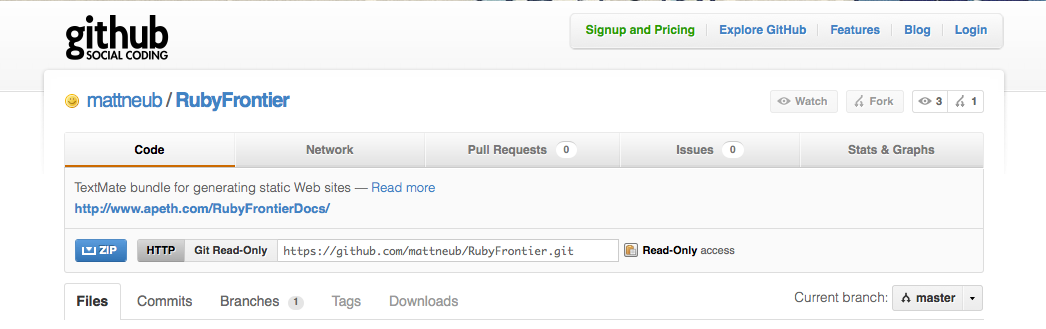
\includegraphics[width=0.7\textwidth]{./images/rubyfrontier-github.png}
\caption{\label{rubyfrontier-github}RubyFrontier auf GitHub}
\end{figure}


Mit einem einfachen Doppelklick kann die Datei auf dem Rechner entpackt werden. Man erhält dann ein ReadMe als Markdown-Datei (was Markdown ist, erfahren Sie später) und dann das eigentliche RubyFrontier-Paket als ein TextMate-Bundle (mit der Endung .tmbundle).

\begin{figure}[h!]
\centering
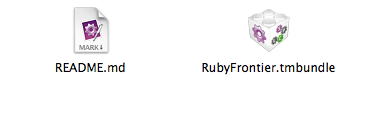
\includegraphics[width=0.7\textwidth]{./images/rubyfrontier-tmbundle.png}
\caption{\label{rubyfrontier-tmbundle}Die ausgepackte Installation}
\end{figure}

Ein Doppelklick auf das TextMate-Bundle installiert es. Wenn alles gut gegangen ist, öffnet sich TextMate mit dem Bundle-Editor und zeigt Ihnen was alles installiert wurde.

\begin{figure}[h!]
\centering
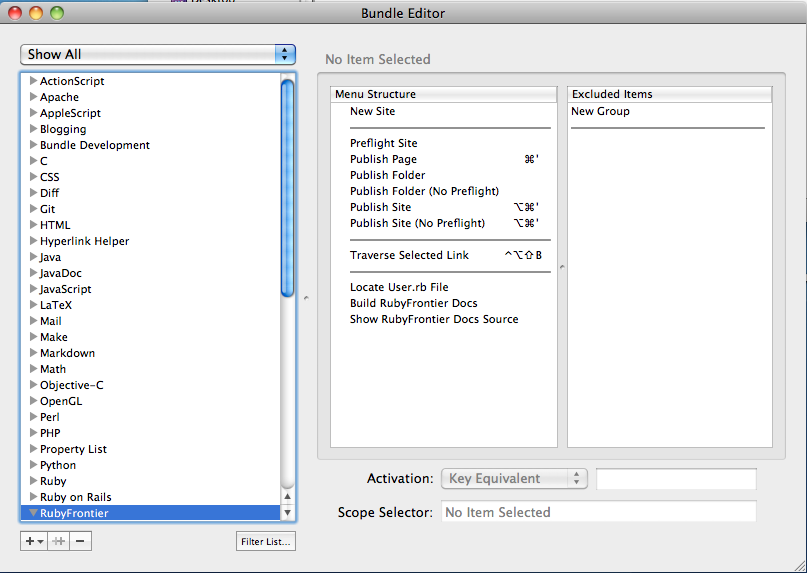
\includegraphics[width=0.7\textwidth]{./images/ruby-frontier-bundle-editor.png}
\caption{\label{ruby-frontier-bundle-editor}RubyFrontier im Bundle-Editor}
\end{figure}

Was zu tun ist, wenn die Installation danebengeht, kann ich Ihnen leider nicht sagen. Ich habe RubyFrontier schon dutzendfach auf diversen Rechnern installiert und bisher ist alles glattgegangen. Hoffen wir also einfach, daß es bei Ihnen genau so ist.

RubyFrontier ist nun fertig installiert. Doch bevor Sie zum ersten Mal loslegen, zügeln Sie Ihre Neugier und beenden TextMate erst einmal wieder und öffnen es dann neu.
\section{Die erste Website}
\label{sec-1-2-2}


Denn bevor Sie wirklich eine neue Website mit RubyFrontier anlegen
können, müssen noch einige Vorarbeiten erledigt werden. Erstellen Sie
zuerst einen Ordner, der alle ihre RubyFrontier-Projekte enthalten
soll und nennen Sie ihn irgendwie, zum Beispiel myRubyFrontierSites.


Tip: Wenn Sie über einen Dropbox-Account verfügen, können Sie diesen
Ordner auch in ihrer Dropbox anlegen. Sie können dann mit ihren
Dateien auf allen Rechnern arbeiten, die mit Ihrer Dropbox verbunden
sind (vorausgesetzt, auf ihnen ist ebenfalls TextMate und RubyFrontier
installiert).


Jetzt öffnen Sie TextMate wieder. Falls Sie Ihre Version so
konfiguriert haben, daß der Editor beim Öffnen kein Textfenster (weder
ein leeres noch das zuletzt benutzte) öffnen soll, öffnen Sie eines,
weil sonst die RubyFrontier-Befehle nicht aufgerufen werden können.


Nun gehen sie in das Menü Bundles und wählen RubyFrontier > New Site
aus. Eventuell besteht TextMate darauf, daß Sie vorher Ihr leeres
Textfenster sichern müssen. Tun Sie der Software diesen gefallen und
sichern Sie es irgendwo ab, wo Sie es leicht wiederfinden und
wegwerfen können (das dürfte bei den meisten von Ihnen der
Schreibtisch sein). Den folgenden Dialog navigieren Sie in den soeben
angelegten Ordner myRubyFrontierSite (oder wie immer Sie ihn genannt
haben) und legen dort einen neuen Ordner an. Ich habe ihn aus
naheliegenden Gründen tutorial genannt.

\begin{figure}[h!]
\centering
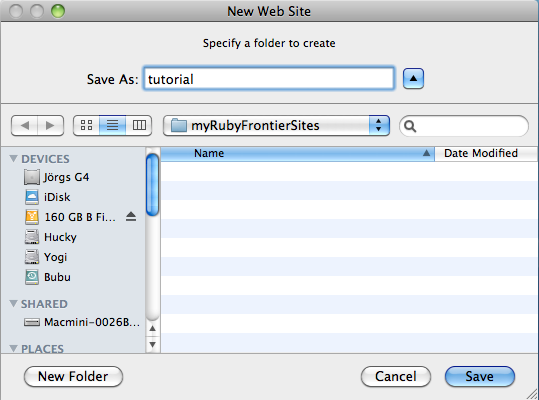
\includegraphics[width=0.7\textwidth]{./images/neuer-source-folder.png}
\caption{\label{neuer-source-folder}Dialog um eine neue Webseite anzulegen}
\end{figure}

Und voilà, schon öffnet sich ein Projekt-Fenster, das Ihnen einen
frisch generierten Ordner mit vielen Dateien, also Ihr neues Projekt,
zeigt:

\begin{figure}[h!]
\centering
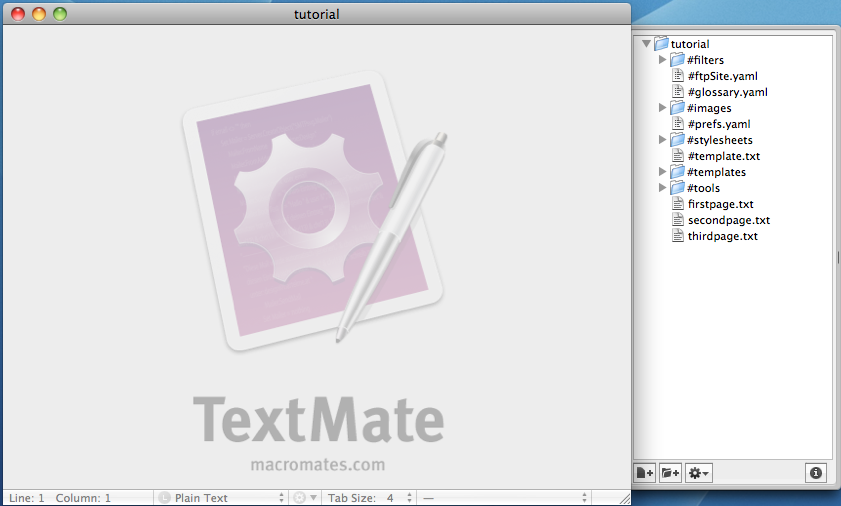
\includegraphics[width=0.7\textwidth]{./images/neues-projekt.png}
\caption{\label{neues-projekt}Frisch angelegtes RubyFrontier-Projekt}
\end{figure}

Bevor Sie weitermachen, sollten Sie noch etwas erledigen, was sonst im
Eifer des Gefechts leicht untergeht: Sichern Sie Ihr frisch angelegtes
Projekt. Dazu gehen Sie in TextMate in das Menü File und dann zu Save
Project. Legen Sie die Projektdatei oberhalb Ihres frisch angelegten
Tutorial-Ordners, aber im Ordner myRubyFrontierSites ab.

\begin{figure}[h!]
\centering
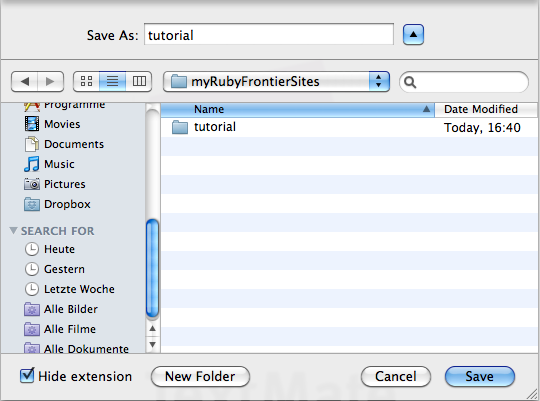
\includegraphics[width=0.7\textwidth]{./images/projekt-sichern.png}
\caption{\label{projekt-sichern}Das Projekt sichern}
\end{figure}


Nennen Sie es wie Ihr Projekt, also tutorial. Das ist nicht zwingend
vorgeschrieben, aber es erleichtert bei vielen Projekten die Übersicht
ungemein. Ihr frisch angelegter Projektordner sollte also so aussehen:

\begin{figure}[h!]
\centering
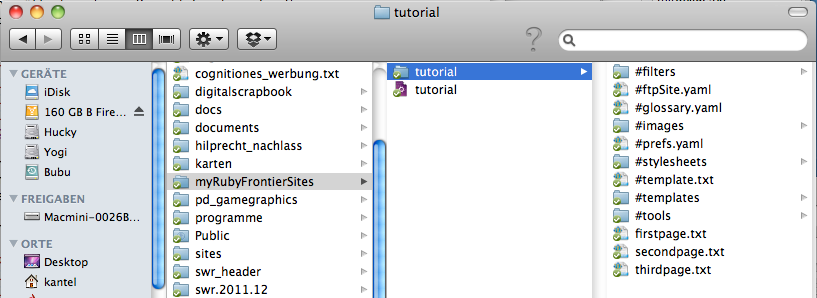
\includegraphics[width=0.7\textwidth]{./images/projektstruktur-1.png}
\caption{\label{projektstruktur-1}RubyFrontier-Projektstruktur}
\end{figure}

Als Letztes ist eines noch zu erledigen: Öffnen Sie die
Datei \#ftpSite.yaml und ändern Sie sie wie folgt:



\begin{verbatim}
:folder: ~/Desktop/tutorial
:method: file
:isLocal: true
\end{verbatim}

Unter :folder: wählen Sie einfach den Ordner aus, in dem Sie Ihre
fertigen Webseiten ablegen möchten. Für’s erste reicht der
Schreibtisch, später werde ich Ihnen andere Alternativen vorschlagen
und Ihnen auch erklären, was der merkwürdige Lattenzaun (\#, auch
Doppelkreuz genannt) bedeutet, der dieser und anderen Dateien und
Ordner vorsteht, bedeutet.


Gratuliere! Sie haben Ihr erstes RubyFrontier-Projekt erfolgreich
angelegt. Ab jetzt können Sie Ihr Projekt einfach öffnen, in dem Sie
auf die Projektdatei klicken.
\subsection{Jetzt aber …}
\label{sec-1-2-2-1}


Nun da Sie die Vorarbeiten erledigt haben, sind Sie endlich in der
Lage, Ihre erste Website mit RubyFrontier zu erstellen. Daher öffnen
Sie mit einem Doppelklick auf die Projektdatei tutorial TextMate
erneut und löschen erst einmal die Dateien firstpage.txt,
secondpage.txt und thirdpage.txt. Dies sind englischsprachige
Beispieldateien, die Sie nicht mehr benötigen. Dafür legen wir eine
Datei index.txt auf der obersten Ebene im tutorial-Ordner an, in die
Sie Folgendes hineinschreiben:



\begin{verbatim}
#title "Startseite"

<h1>Meine erste Website: <%= title %></h1>

<p>
Hallo Welt! Grüße von RubyFrontier.</p>
\end{verbatim}

Jetzt achten Sie darauf, daß diese Datei im Hauptfenster zu sehen ist
(den Fokus besitzt) und wählen im Menü Bundle den Punkt RubyFrontier >
Publish Page aus. Wenn Sie sich nicht irgendwo vertippt haben, sollte
— nachdem TextMate eine Zeitlang gearbeitet hat — Ihr Standard-Browser
aufgehen und ihnen folgende Seite zeigen:

\begin{figure}[h!]
\centering
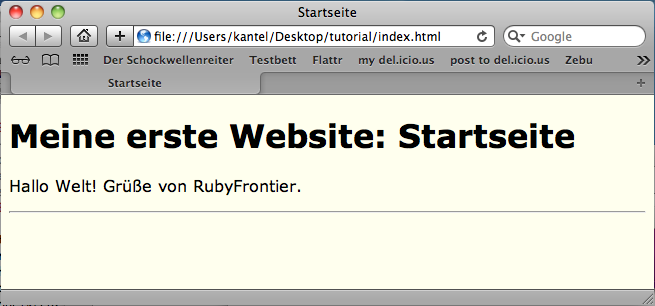
\includegraphics[width=0.7\textwidth]{./images/index.png}
\caption{\label{index01}Ihre erste, mit RubyFrontier erstellte Seite}
\end{figure}


Wenn Sie mit Bildern arbeiten, benötigen Sie die Ruby-Bibliothek
dimensions, die Sie auf Ihrem Mac ganz einfach mit nachladen
können. Dazu öffnen Sie ein Terminalfenster und tippen dort


\begin{verbatim}
sudo gem install dimensions
\end{verbatim}

ein. Sie werden nach Ihrem Passwort gefragt und kurz danach ist die
Bibliothek installert.


Je nach Umfang Ihrer Ruby-Installation könnten jedoch noch andere
Ruby-Bibliotheken angemeckert werden, z.B. kramdown, SASS, LESS, HAML
und lib/xml. Obwohl Sie für die Arbeit in diesem Buch eigentlich nur
noch kramdown wirklich benötigen, schadet es nicht, die anderen
fehlenden auch zu installieren. Denn LESS resp. SASS und auch die
lib/xml könnten für spätere Aufgaben durchaus nützlich sein. Dazu
öffnen Sie das Terminalfenster und tippen zum Beispiel ein:


\begin{verbatim}
sudo gem install kramdown
\end{verbatim}

Sie werden aufgefrodert, Ihr Admin-Passwort einzugeben (das ist das,
das Sie bei vielen anderen Programm-Installationen und
Betriebssystem-Updates ebenfalls eingeben müssen) und dann läuft die
Installation automatisch ab.


Genau so verfahren Sie mit LESS, SASS oder HAML:


\begin{verbatim}
sudo gem install less
sudo gem install sass
sudo gem install haml
\end{verbatim}

lib/xml ist eine Besonderheit, da der Name der Bibliothek hier anders
eingegeben werden muß:



\begin{verbatim}
sudo gem install libxml-ruby
\end{verbatim}

Außerdem wird Ihnen RubyFrontier im Meldungsfenster noch empört
mitteilen, daß die Datei user.rb nicht gefunden würde. Auch diese
Datei wird nicht unbedingt benötigt (hier können Sie z.B. Makros
ablegen, die für mehrere RubyFrontier-Projkete Verwendung finden
sollen), aber falls Sie die Meldung stört, legen Sie einfach eine
Datei user.rb an und teilen Sie RubyFrontier über das Menü Bundels ->
RubyFrontier -> Locate User.rb File mit, wo Sie diese angelegt
haben. Theoretisch kann das überall auf Ihrer Festplatte sein und Sie
können das auch jederzeit ändern, ich empfehle Ihnen, die Datei im
Ordner myRubyFrontierSites auf oberster Ebene abzulegen, also dort, wo
auch schon Ihre TextMate-Projektdatei liegt.


Doch jetzt wieder die Frage: Was ist eigentlich passiert? Die erste
Zeile mit der merkwürdigen Bezeichnung


\begin{verbatim}
#title "Startseite"
\end{verbatim}

ist eine Direktive. Sie weist RubyFrontier an, daß unter dem Namen
title der Wert Startseite abzuspeichern ist. Jede neue Seite muß die
Direktive title enthalten und diese sollte aus Gründen, die ich Ihnen
weiter unten erläutere, eindeutig sein, d.h. keine Seite darf den
gleichen Titel wie eine andere besitzen.


Bevor RubyFrontier mit dem Prozeß des Herausschreibens beginnt,
sammelt es diese und andere Direktiven im Hauptspeicher und kann dann
darauf zugreifen. Genau das haben Sie mit der Zeichenfolge


\begin{verbatim}
<h1>Meine erste Website: <%= title %></h1>
\end{verbatim}

getan. An dieser Stelle wird der Inhalt der title-Direktive, in diesem
Falle also »Startseite«, eingesetzt. Auch wenn Direktiven weit
mächtiger sind, können sich Programmierer diese erst einmal als eine
Art Variable vorstellen.


Der Rest ist simples HTML. RubyFrontier kann auch mit anderen
Markup-Sprachen (z.B. Markdown) umgehen, wie ich Ihnen in einem
späteren Abschnitt zeigen werde.


Der Befehl »Publish Page« hat RunyFrontier angewiesen, den Text als
HTML-Datei herauszuschreiben, zu »rendern«, das heißt aus diesem Text
eine HTML-Seite für das Web zu erstellen. Die Seite liegt, wenn Sie
meinen Empfehlungen gefolgt sind, auf Ihrem Schreibtisch im Ordner
tutorial und heißt index.html. Es ist eine stinknormale
HTML-Seite. Sie können Sie mit jedem beliebigen Texteditor öffnen und
sich anschauen, Sie könnten sie aber auch mit einem (S)FTP-Client
Ihrer Wahl auf einem Server ablegen.
\subsection{Templates}
\label{sec-1-2-2-2}


Doch wo kommt eigentlich der Rest des HTML her, das RubyFrontier um
Ihre Websiete herum gebastelt hat? Um das herauszubekommen, öffnen Sie
doch einfach in TextMate die Datei \#template.txt und Sie werden dieses
sehen:



\begin{verbatim}
<%= pageheader() %>
<p id="bodytext"></p>
<hr />
<%= nextprevlinks() %>
<%= pagefooter() %>
\end{verbatim}

Die erste Zeile sorgt dafür, daß das HTML vor Ihrem Text erzeugt wird,
die letzte Zeile bringt das HTML nach Ihrem Text. Und der Eintrag


\begin{verbatim}
<p id="bodytext"></p>
\end{verbatim}

sorgt dafür, daß an dieser Stelle Ihr Text erscheint. Danach wird noch
eine horizontale Linie erzeugt und ein Makro aufgerufen, das Links zu
den vorherigen und nachfolgenden Seiten erzeugt, falls Sie das
wünschen. Momentan benötigen Sie diese Zeile noch nicht, daher können
Sie sie gefahrlos löschen (es stört aber auch nicht wirklich, wenn Sie
sie stehen lassen.


Das heißt also: Jedesmal, wenn Sie eine Seite herausrendern, sucht
sich RubyFrontier das »zuständige« Template und bringt dieses mit
Ihrem zu rendernden Text zusammen.


Natürlich können Sie auch Templates ändern. Vermerken Sie doch einfach
einmal stolz in ihrem Template, womit Sie die Seite herausgeschrieben
haben


\begin{verbatim}
<%= pageheader() %>
<p id="bodytext"></p>
<hr />
<p style="font-size:small;">
Diese Seite wurde mit RubyFrontier erstellt.</p>
<%= pagefooter() %>
\end{verbatim}

und rendern dann Ihre Datei index.txt erneut heraus. Sie sollte jetzt
so aussehen:

\begin{figure}[h!]
\centering
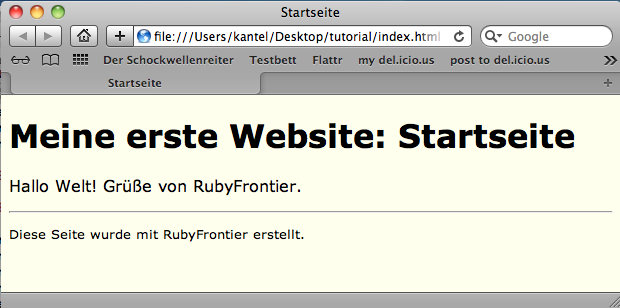
\includegraphics[width=0.7\textwidth]{./images/index02.png}
\caption{\label{index02}Änderung am Template}
\end{figure}


Die Zeilen


\begin{verbatim}
<%= pageheader() %>
<%= pagefooter() %>
\end{verbatim}

sind, wie schon erwähnt, Makroaufrufe. Makroaufrufe stehen immer in
spitzen Klammern und Prozentzeichen. Und das Gleichheitszeichen
bedeutet, daß das Makro einen Wert (in der Regel einen String, also
Text) zurückliefert. Makros ohne das Gleichheitszeichen berechnen zwar
auch irgendetwas, haben aber nur indirekt Einfluß auf die
herausgeschriebenen Seiten.
\subsection{Ein erstes Makro}
\label{sec-1-2-2-3}


Das ist zwar schon etwas, aber eigentlich noch langweilig. Häufig
steht im Footer einer Seite, wann das letzte Update passiert
ist. Dafür schreiben wir uns ein Makro. Makros sind kleine
Ruby-Programme, die irgendetwas zurückliefern, was Sie in Ihre
Webseite einbauen wollen. Üblicherweise werden Makros im \#tools-Ordner
abgelegt und haben die Dateiendung .rb. Also öffnen Sie den
Tools-Ordner und legen darin eine Datei mit dem Namen clocknow.rb
an. Und in diese Datei schreiben Sie folgendes kleine Ruby-Skript:


\begin{verbatim}
def clocknow()
  t = Time.new
  t.strftime("%d.%m.%Y, %H:%M Uhr")
end
\end{verbatim}

Makro-Dateien haben üblicherweise den gleichen Namen wie die Funktion,
die daraus aufgerufen werden soll — obwohl das nicht zwingend
ist. Aber es erleichtert die Übersicht. Den Namen clocknow habe ich
als Reminiszens an eine gleichnamige Frontier-Funktion
gewählt. Ruby-Funktionen liefern im Default-Fall den Wert der letzten
Programmzeile (vor dem end) zurück, ein explizites return ist nicht
erforderlich. Die Funktion ist recht einfach: Erst weisen Sie der
Variablen t die aktuelle Zeit zu und dann formatieren Sie diese, so
daß sie den deutschen Gepflogenheiten, also dd.mm.YYYY, HH:MM
entspricht. Die vorletzte Zeile in Ihrem Template ändern Sie auch noch
(der Zeilenumbruch dient nur der besseren Lesbarkeit):


\begin{verbatim}
<p style="font-size:small;">Diese Seite wurde mit RubyFrontier erstellt.
   Letzte Änderung: <%= clocknow() %></p>
\end{verbatim}

Und schon steht nach jedem Herausschreiben die aktuelle Uhrzeit auf
Ihrer Seite.

\begin{figure}[h!]
\centering
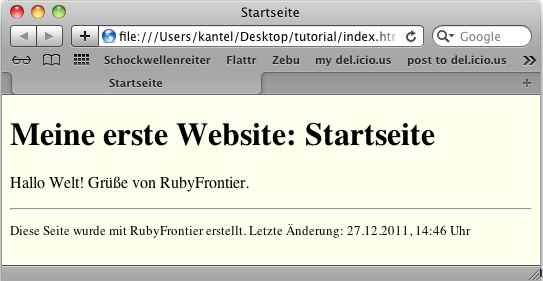
\includegraphics[width=0.7\textwidth]{./images/clocknow.png}
\caption{\label{clocknow}Seite mit aktueller Uhrzeit}
\end{figure}


Dieses Makro wäre zum Beispiel auch ein Kandidat für ein Makro, das
Sie in der oben angelegten Datei user.rb ablegen könnten, da Sie die
Uhrzeit sicher auch in anderen Projekten benötigen. Für die weitere
Arbeit an diesem Tutorial lassen Sie sie jedoch bitte erst einmal
im \#tools-Ordner.
\chapter{Die Benutzeroberfläche von RubyFrontier}
\label{sec-1-3}


\begin{figure}[h!]
\centering
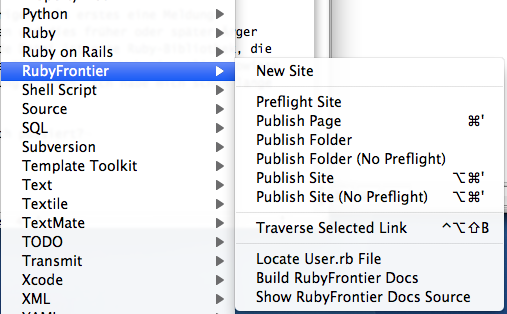
\includegraphics[width=0.7\textwidth]{./images/rubyfrontier-im-bundles-menue.png}
\caption{\label{rubyfrontier-im-bundles-menue}RubyFrontier im Bundles-Menü}
\end{figure}

RubyFrontier ist ja bekanntlich ein TextMate Bundle und so sind die
RubyFrontier Befehle natürlich über das Menü Bundle zu
erreichen. Fahren Sie mit der Maus in diesem Menü über den Eintrag
RubyFrontier, so öffnet sich ein Untermenü mit etwas mehr als zwei
Handvoll (genauer: elf) Befehlen. Es sind dies:

\begin{itemize}
\item New Site
\item Preflight Site
\item Publish Page
\item Publish Folder
\item Publish Folder (No Preflight)
\item Publish Site
\item Publish Site (No Preflight)
\item Traverse Selected Link
\item Locate User.rb File
\item Build RubyFrontier Docs
\item Show RubyFrontier Docs Source
\end{itemize}

Das gleiche Menü (nur in kleinerer Schriftgröße) erhalten Sie auch,
wenn Sie auf das kleine Zahnrädchen in der Fußzeile des Fensters
klicken (es ist die dritte Spalte von links):

\begin{figure}[h!]
\centering
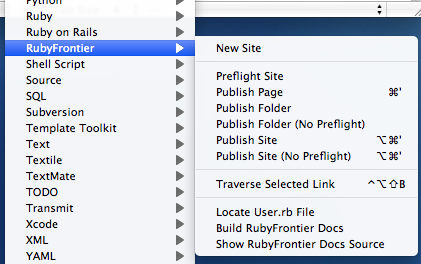
\includegraphics[width=0.7\textwidth]{./images/rubyfrontier-in-textmate-fusszeile.png}
\caption{\label{rubyfrontier-in-textmate-fusszeile}RubyFrontier in der Fußzeile des Textfensters}
\end{figure}

Welche von beiden Möglichkeiten Sie bevorzugen, ist
Geschmackssache. Bei mir ist die Fußzeile der kürzere Mausweg und
daher benutze ich fast immer diese. Aber da es für die wichtigsten
Menüs immer auch Tastaturkürzel gibt, benutze ich die Menüs so gut wie
gar nicht, sondern rufe RubyFrontier immer über die Tastatur auf.


Die Menüpunkte bedeuten im Einzelnen (auf die Preflight-Menüs komme
ich später im Zusammenhang mit dem Glossary-Mechanismus von
RubyFrontier zu sprechen):


\begin{itemize}
\item New Site: Diesen Befehl haben Sie schon am Anfang kennengelernt,
  damit legen Sie ein komplett neues RubyFrontier-Projekt mit all
  seinen Dateien und Ordnern an.
\end{itemize}


\begin{itemize}
\item Publish Page schreibt eine einzelne Seite heraus.
\item Publish Folder schreibt alle Seiten eines Unterordners und der
  Ordner darunter heraus. Diesen Punkt hat Matt Neuburg auf meine
  Anregung in RubyFrontier eingebaut. Denn wie ich weiter oben schon
  einmal schrieb, hatte ich versucht, eine große Sammlung mithilfe von
  RubyFrontier zu publizieren. Und es kann die zum Rendern notwendige
  Zeit doch erheblich verkürzen, wenn man nur Teilbäume
  herausschreiben muß.
\end{itemize}


\begin{itemize}
\item Publish Site ist der Befehl, um alle Dateien eines Projektes
  herauszuschreiben.
\end{itemize}


\begin{itemize}
\item Traverse Selected Link versucht, einen selektierten (internen) Link
  zu interpretieren und die entsprechende Seite in TextMate zu
  öffnen. Dieser Befehl kann bei einem großen Projekt sehr hilfreich
  sein, wenn Sie zum Beispiel herausfinden wollen, was eigentlich noch
  mal auf der Seite stand, die sich hinter diesem Link verbirgt.
\end{itemize}


\begin{itemize}
\item Locate User.rb File: User.rb ist die Datei, in der Sie
  projektübergreifend Ruby-Makros für ihre Webseiten unterbringen. Im
  Regelfalle nutzen Sie sie nicht, wenn Sie mit RubyFrontier beginnen,
  aber irgendwann kommt der Punkt, wo Sie über eine Sammlung
  nützlicher Skripte verfügen, die Sie für alle Ihre Sites parat haben
  wollen.
\end{itemize}


\begin{itemize}
\item Build RubyFrontier Docs rendert Matt Neuburgs
  RubyFrontier-Dokumentation auf Ihrem Schreibtisch heraus und öffnet
  sie anschließend im Browser. Sollten Sie mindestens einmal aufrufen,
  damit Sie sie zur Verfügung haben, auch wenn Sie offline arbeiten.
\end{itemize}


\begin{itemize}
\item Show RubyFrontier Docs Source öffnet die RubyFrontier-Dokumentation
  als RubyFrontier-Projekt in TextMate. Das ist — wenn Sie mit
  RubyFrontier ein wenig fortgeschritten sind — eines der nützlichsten
  Hilfen überhaupt. Denn hier können Sie nachschauen, wie der Meister
  seine Probleme gelöst hat.
\end{itemize}


Ja, und das letzte »GUI«-Element von RubyFrontier ist das
Meldungsfenster von TextMate:

\begin{figure}[h!]
\centering
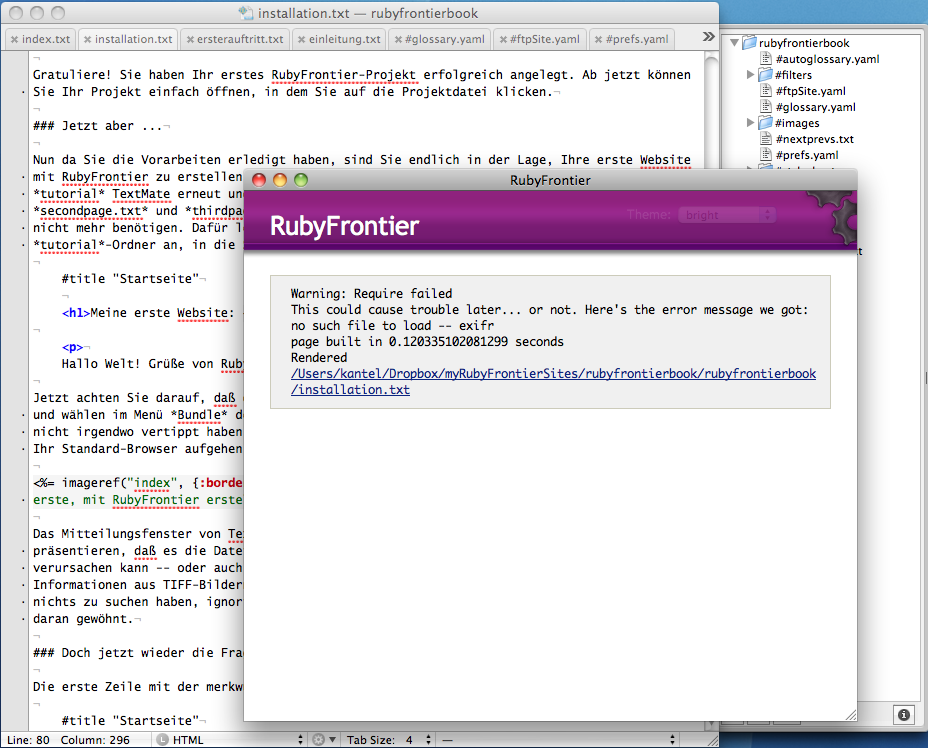
\includegraphics[width=0.7\textwidth]{./images/rubyfrontier-meldungsfenster.png}
\caption{\label{rubyfrontier-meldungsfenster}RubyFrontier-Meldungsfenster}
\end{figure}


Hier stehen — wenn etwas schiefläuft — auch die mehr oder weniger
aussagekräftigen Informationen über den gefundenen Fehler. Es ist ein
oft sehr hilfreiches, aber schnittstellentechnisch etwas
benutzerunfreundlich gelöstes Feature. Denn man muß nach jedem
Durchlauf dieses Fenster erst einmal wegklicken (oder sonstwie dafür
sorgen, daß das eigentlich Textfenster, mit dem man arbeitet, den
Fokus bekommt), bevor man weiterarbeiten kann. Aber das ist ein
Feature von TextMate und kann nicht dem Programmierer von RubyFrontier
angelastet werden.
\part{Webseiten bauen mit RubyFrontier}
\label{sec-2}
\chapter{Eine erste Website mit RubyFrontier}
\label{sec-2-1}
\section{Ihr Hundesportverein im Web}
\label{sec-2-1-1}


Nachdem Sie nun die Grundlagen der Webseiten-Erstellung mit
RubyFrontier kennengelernt haben, werden wir nun in medias res gehen
und eine erste »echte« Website erstellen. Dazu stellen Sie sich bitte
vor, Sie sind Mitglied im Hundesportverein Flughund e.V. und der
Vorstand hat Sie beauftragt, eine Homepage für Ihren Verein zu
erstellen. Vermutlich war Ihr erster Gedanke dann, ein vollständiges
Content Management System (CMS), wie z.B. Drupal, Joomla! oder das
sehr populäre WordPress einzusetzen, in dem dann alle
Vereinsmitglieder mitschreiben und Inhalte einstellen können. Aber
glauben Sie mir: Sie tun es nicht. Ich habe jahrelang die Webseiten
(m)eines Hundesportvereins gepflegt. Sie werden Emails mit — im
schlimmsten Falle — Word-Dateien bekommen, die eventuell sogar noch
liebevoll gestaltet sind und diese sollen Sie dann genau so ins Web
stellen.


Und das ist nicht Hundesportverein-typisch. In Ihrem Fußball- oder
Eishockeyverein, in Ihrer Bürgerinitiative oder wofür Sie immer eine
Website erstellen wollen oder sollen, wird es nicht anders sein.


Ein CMS ist in solchen Fällen nicht nur ein totaler Overkill, sondern
bedeutet für Sie auch noch mehr Arbeit: Sie müssen Updates einspielen,
die Datenbank pflegen und Sicherheitshinweise beachten. Und daher
können Sie — wenn sowieso alles nur über Ihren Rechner läuft — auch
genau so gut, wenn nicht besser, RubyFrontier dafür benutzen: Keine
Updates, keine Datenbank und keine Sicherheitsprobleme. Und billiger
wird es im Regelfalle auch noch, da Sie für statische Seiten die
günstigste Hosting-Möglichkeit auswählen können. (Das letzte Argument
wird mit Sicherheit den Kassenwart Ihres Vereins überzeugen.)


Sie werden daher jetzt sukzessive die anfangs erstellten Seiten zu
einem kleinen Webauftritt aufbauen. Dazu schreiben Sie erst einmal
etwas in die Startseite (index.txt) hinein.


\begin{verbatim}
#title: "HSV Flughund e.V.: Startseite"

<h1>Willkommen auf den Webseiten des Hundesportvereins Flughund e.V.</h1>
<p>
Der HSV Flughund e.V. ist eine Organisation von Hundesportlern und
Hundeliebhabern. Wir betreiben insbesondere die Hundesportarten Agility,
Obedience und den Turnierhundesport. Auch die Ausbildung von
menschenfreundlichen Familienhunden und verkehrssicheren Begleithunden
wird angestrebt. Jede der Gesundheit der Hunde und ihrer Hundeführer
dienende Aktivität wird unterstützt. Darüberhinaus leistet der Verein
Aufklärungsarbeit in der Öffentlichkeit zur artgerechten Hundehaltung
und -erziehung. Der HSV Flughund e.V. setzt sich aktiv für Tierschutz,
Umweltschutz und Jugendarbeit ein.</p>
\end{verbatim}

Schlagen Sie mich bitte nicht wegen des Textes. Er ist zum großen Teil
der Satzung eines real existierenden Hundesportvereins entnommen. Aber
darauf kommt es ja auch nicht an. Rendern Sie den Text heraus und Sie
sollten eine Webseite erhalten, die ungefähr so aussieht:

\begin{figure}[h!]
\centering
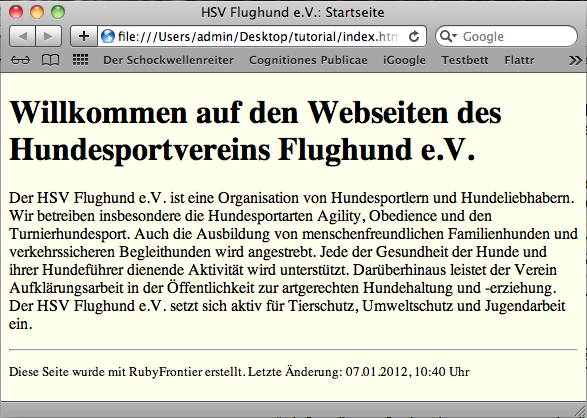
\includegraphics[width=0.7\textwidth]{./images/flughund01.png}
\caption{\label{flughund01}Screenshot 1: HSV Flughund e.V.}
\end{figure}


Das ist zwar schon etwas, aber noch nicht wirklich weltbewegend. Mich
— und vielleicht auch Sie — ie blaßgelbe Farbe des
Hintergrunds. Um diese zu ändern, öffnen Sie doch einfach die
Datei \#prefs.yaml. Dort steht nur folgender Eintrag:


\begin{verbatim}
--- 
:bgcolor: FFFFEE
\end{verbatim}

YAML ist eine vereinfachte Auszeichnungssprache, die sowohl von Ruby
leicht zu parsen als auch von Menschen zu lesen ist und daher hat Matt
Neuburg sie ausgewählt, um einige Voreinstellungen für Ihre Webseiten
ablegen zu können. Ändern Sie also einfach die Hintergrundfarbe
bgcolor nach weiß:


\begin{verbatim}
---
:bgcolor: ffffff
\end{verbatim}

Die Farbdarstellung ist eine Kodierung der Hexwerte, wie sie in HTML
üblich ist. Das dabei normalerweise nötige führende Doppelkreuz
kann/muß entfallen, statt \#ffffff schreiben Sie also einfach
ffffff. (Und wie Sie gesehen haben, bevorzuge ich die Kleinschreibung
der Hexwerte, das ist allerdings völlig egal, der Browser
interpretiert das schon richtig.)

Wenn Sie jetzt die Startseite erneut herausschreiben lassen, hat sie
eine weiße Hintergrundfarbe.

Die prefs.yaml ist der Ort, in dem Sie viele weitere Voreinstellungen
ablegen können. Ich werde im Laufe dieser Einführung noch häufiger
darauf zurückkommen.
\subsection{Ein neuer Pageheader}
\label{sec-2-1-1-1}


Was Sie vermutlich stört, ist das der Titel der Startseite HSV Flughund e.V.: Startseite heißt. Ich habe das so angelegt, weil ich möchte, daß in der Kopfleiste des Browserfenster, in dem immer der komplette Seitentitel steht, auch der Name des Vereins auftaucht. Denn dieser Seitentitel ist für die meisten Suchmaschinen, speziell für Google sehr relevant. Aber es macht die Titelei doch sehr unhandlich. RubyFrontier holt sich den Pageheader irgendwo aus den Tiefen seines Quellcodes, aber es gibt natürlich Möglihckeiten, hier einzugreifen.

Die einfachste Möglichkeit, einen eigenen Pageheader zu bekommen, ist es, eine Datei namens \#pageheader.txt im Wurzelverzeichnis anzulegen, also dort, wo zum Beispiel auch die \#prefs.yaml oder die \#ftpSite.yaml zu finden ist. Sie sollte so aussehen:


\begin{verbatim}
<!DOCTYPE html PUBLIC "-//W3C//DTD XHTML 1.0 Transitional//EN"
"http://www.w3.org/TR/xhtml1/DTD/xhtml1-transitional.dtd">
<html xmlns="http://www.w3.org/1999/xhtml" xml:lang="de" lang="de">
<head>
    <%= metatags() %>
    <%= linkstylesheets() %>
    <%= linkjavascripts() %>
    <title><%= sitetitle %>: <%= title %></title>
</head>
<%= bodytag() %>
\end{verbatim}

Bis auf zwei Ausnahmen entspricht dieser Pageheader exakt dem
Pageheader, der von RubyFrontier per Default herausgeschrieben
ist. Die erste Ausnahme steckt in der dritten Zeile, hier habe ich dem
HTML-Tag noch mitgeteilt, daß diese Seite in deutscher Sprache
geschrieben ist. Dies wird häufig vergessen, ist aber ein wichtiger
Anhaltspunkt für Suchmaschinen:


\begin{verbatim}
<html xmlns="http://www.w3.org/1999/xhtml" xml:lang="de" lang="de">
\end{verbatim}

Und dann habe ich in den <title>-Tag noch den Aufruf <\%= sitetitle \%>
eingefügt. Das ist eine selbsterstellte Direktive und Sie müssen
RubyFrontier nun noch bekanntmachen, daß diese Direktive einen Wert
besitzt. Die geeignetste Stelle ist dafür wieder die Datei \#prefs.yaml
Also fügen Sie dort folgende Zeile ein:


\begin{verbatim}
:sitetitle: 'HSV Flughund e.V.'
\end{verbatim}

Nun können Sie den \#title in der index.txt auf “Startseite”
verkürzen. Wenn Sie nun die Seite wieder herausschreiben, werden Sie
feststellen, daß — wie erwartet — der HSV Flughund e.V. dennoch in der
Titelleiste des Brwosers erscheint. Und das wird er auch in allen
Seiten, die Sie noch erstellen werden.

Spätestens dann, wenn Sie viel mit JavaScript arbeiten, werden Sie
froh sein, daß RubyFrontier Ihnen diverse Möglichkeiten bietet, einen
eigenen Pageheader zu erzeugen. Ich werde später noch darauf
zurückkommen.

Was bedeuten nun die anderen Zeilen im Pageheader? <\%= metatags() \%>
schreibt diese beiden Zeilen heraus:


\begin{verbatim}
<meta http-equiv="content-type" content="text/html; charset=utf-8" />
<meta name="generator" content="RubyFrontier" />
\end{verbatim}

Die erste Zeile sollten Sie nur ändern, wenn Sie wirklich wissen, was
Sie tun (ihre Seite zum Beispiel komplett auf chinesisch ist). Die
zweite Zeile gibt RubyFrontier Kredit. Das ist nicht nur eine
Spielerei — vielleicht will Matt Neuburg mal wissen, wieviele Seiten
mit seiner Software es im Netz gibt — und sollte daher, wenn es keine
Gründe gibt, die dagegen sprechen, auch nicht geändert werden.


Die nächsten beiden Zeilen machen momentan noch gar nichts, da Sie in
ihrer Site bisher wegerr etwas mit JavaScript noch mit Cascading Style
Sheets (CSS) angestellt haben. Zumindest das letztere wird sich aber
gleich ändern.

Der letzte Unbekannte ist noch der <\%= bodytag() \%>-Aufruf. Er
schreibt per Default nur <body> heraus, kann aber noch andere
Parameter, wie zum Beispiel die Text- oder die Linkfarbe,
übernehmen. Dies ist jedoch veraltet, da man dies heutzutage im
Regelfalle mit Stylesheets erledigt und sollte daher nur angewendet
werden, wenn es Gründe dafür gibt. Ein Grund wäre zum Beispiel, daß
man auf jeden Fall ein bestimmtes Aussehen erreichen will, auch wenn
die Stylesheets nicht geladen oder interpretiert werden.
\subsection{Text mit Stil}
\label{sec-2-1-1-2}


Wenn Sie den \#stylesheets-Ordner öffnen, werden Sie feststellen, daß
es dort schon zwei CSS-Dateien gibt (s1.css und s2.css). Sie sind aus
didaktischen Gründen dort, Sie benötigen sie aber nicht, daher können
Sie sie einfach wegwerfen. Legen Sie stattdessen in diesem Ordner eine
Datei namens default.css an (sie könnte auch irgendwie anders heißen,
es ist einfach der Name, den ich für die Default-Stylesheet-Datei
bevorzuge). Und dort schreiben Sie folgendes hinein:


\begin{verbatim}
body {
    font-family: Verdana, sans-serif;
    font-size: 12px;
}

h1 {
    font-size: 18px;
}

.small {
    font-size: 10px;
}
\end{verbatim}

Es ist ein minimalistisches Stylesheet, das ich Ihnen hier
anbiete. Aber einmal ist dies kein Lehrbuch über CSS und zum anderen
will ich Ihnen erst einmal auch nur das Prinzip erläutern. Wenn Sie
jetzt die Seite neu herausschreiben, werden Sie feststellen, daß
nichts Neues passiert. RubyFrontier weiß nämlich noch nicht, welches
Stylesheet es nutzen soll, dies müssen Sie der Software erst noch
mitteilen. Und die naheliegendste Stelle, wo dies geschehen kann, ist,
was Sie sicher schon geahnt haben, wieder die Datei \#prefs.yaml. Fügen
Sie ihr einfach noch eine weitere Zeile hinzu:


\begin{verbatim}
:linkstylesheets: [default]
\end{verbatim}

Außerdem sollten Sie im Template noch etwas ändern. Der Tag


\begin{verbatim}
<p style="font-size:small;">
\end{verbatim}

sollte in


\begin{verbatim}
<p class="small">
\end{verbatim}

umgewandelt werden, da Sie den Stil dafür ja nun auch in ihrem
Stylesheet festgelegt haben.

\begin{figure}[h!]
\centering
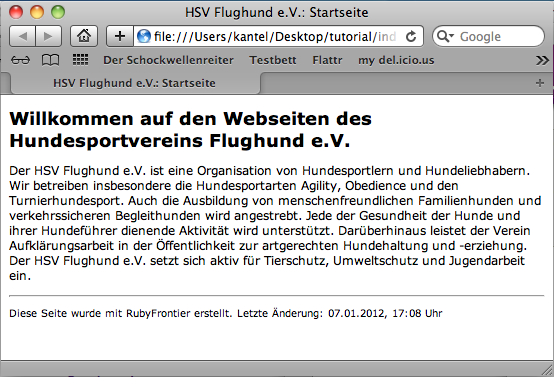
\includegraphics[width=0.7\textwidth]{./images/flughund02.png}
\caption{\label{flughund02}Screenshot 2: HSV Flughund e.V. mit Stil}
\end{figure}


Okay, die Schrift ist vielleicht ein wenig arg klein geraten, aber ich
wollte ja auch, daß Sie einen Unterschied zur Seite ohne Stylesheet
sehen. Sie sind ausdrücklich eingeladen, ein wenig mit den Parametern
zu spielen, damit Sie ein Gefühl dafür bekommen, wie sich diese auf
das Aussehen der Seite auswirken.


Stylesheets können ja bekanntlich auf zweierlei Arten eingebunden
werden: Einmal kann man ein Stylesheet direkt in den <head> einer
HTML-Seite schreiben und einmal kann man es mit Link auf eine externe
CSS-Datei dazulinken. Beide Methoden haben ihre Vor- und Nachteile:
Seiten mit eingebundenen Stylesheets laden in der Regel schneller, da
sie keine weitere Datei nachladen müssen. Dies ist bei der heutigen
Geschwindigkeit des Internets jedoch nur noch bei sehr stark
frequentierten Seiten ein Problem, sicher jedoch nicht bei der Seite
Ihres Hundesportvereins.


Bei Seiten mit Links auf externe Stylesheets braucht man dafür auch
nur an dieser einen Stelle etwas ändern, wenn es etwas zu ändern
gibt. Da das Stylesheet bei jedem Aufruf einer Seite nachgeladen wird,
sind die Änderungen — von irgendwelchem Cache-Verhalten des Browsers
mal abgesehen — sofort sichtbar.


Zwar müssen Sie bei RubyFrontier auch nur an einer Stelle ein
engebettetes Stylesheet ändern, damit die Änderungen aber wirksam
werden, müssen Sie alle Seiten neu herausschreiben. Und das kann bei
einem größeren Webauftritt schon etwas dauern. Daher empfehle ich,
nach Möglichkeit auf das Einbetten von Stylesheets zu verzichten. Aber
— wie ich später noch zeigen werde — es kann durchaus Situationen
geben, wo das Einbetten eines Stylesheets die sinnvollere Lösung ist.
\subsection{Wir wollen Bilder!}
\label{sec-2-1-1-3}


\begin{figure}[h!]
\centering

\includegraphics[width 2cm]{./images/hund02.jpg}
\caption{\label{hund02}Sheltie}
\end{figure}


Eine Website ohne Bilder ist wie ein … Fisch ohne Fahrrad. Mindestens!
Und natürlich bietet auch RubyFrontier die Möglichkeit, Bilder
komfortabel einzubinden. Laden Sie sich dazu erst einmal das
nebenstehende Bild eines kleinen Sheltie herunter. Es heißt
hund02.jpeg und der natürliche Ort, in dem RubyFrontier Bilder
abspeichert, ist der \#images-Ordner. Dort sollte bisher nur die Datei
RubyFrontierLogo.png liegen und dort legen Sie nun auch das
Hundebildchen hinein.


Dann geben Sie in der Startseite unter dem ersten Paragraph-Tag (<p>)
folgendes Makro ein:


\begin{verbatim}
<%= imageref("hund02", {:border => "0", :width => "64", :height => "64",
:alt => "Sheltie", :align => "left", :hspace => "8", :vspace => "4"})
%>
\end{verbatim}

Das Makro verlang als erstes den Namen der Datei ohne Endung,
unterstützt werden JPEG-, GIF- und PNG-Bilder, alle anderen Formate
führen zu Fehlermeldungen. Danach folgt eine Liste der Attribute, auf
die Angabe von Höhe und Weite können Sie verzichten, wenn das Bild —
wie hier — in der Originalgröße abgebildet werden soll, RubyFrontier
rechnet diese für Sie aus. Ich habe Sie hier nur beispielhaft
aufgenommen, damit Sie wissen, wie Sie ein Bild verkleinern oder
vergrößern können.


Alle Parameter außer dem Dateinamen sind übrigens optional, aber
manchmal, wie im Falle der Linksbündigkeit, auch notwendig. Wenn der
alt-Parameter fehlt, bastelt sich RubyFrontier einen aus dem
Dateinamen zusammen, da er der einzige Parameter ist, der bei HTML
vorgeschrieben ist. Und RubyFrontier gibt sich große Mühe, valides
XHTML zu erzeugen. Die Reihenfolge der Parameter ist übrigens
beliebig, sie besteht aus einer kommagetrennten Liste mit den
einzelnen Listenpaaren:


\begin{verbatim}
:attribut => "Attributwert"
\end{verbatim}

Menschen wie ich, die Ruby nicht mit der Muttermilch eingesogen haben,
vergessen übrigens häufig den Doppelpunkt vor dem :attribut. Das führt
zu häßlichen Fehlermeldungen, die man als Anfänger nicht immer richtig
interpretiert. Daher achten Sie bitte darauf, diese (und auch die
Kommata) nicht zu vergessen.
\subsection{Ein Wort noch zu den (internen) URLs}
\label{sec-2-1-1-4}


Eine von RubyFrontiers Zielen ist es, eine Website so portabel wie
möglich zu halten. Daher sind alle internen URLs — auch die zu den
Bildern —, die von RubyFrontier generiert werden, relative URLs. Dies
sollte uns jedoch nicht weiter beunruhigen, denn RubyFrontier erledigt
dies gut. Wichtigstes Hilfsmittel dazu ist die
Datei \#autoglossary.yaml, die von RubyFrontier automatisch erzeugt
wird. Diese Datei sollten Sie daher nach Möglichkeit nicht
anfassen. Sie gehört RubyFrontier und nur RubyFrontier.


Sie helfen RubyFrontier auch, wenn Sie alle Dateinamen eindeutig
halten. RubyFrontier kommt zwar auch mit einer zweiten index.txt in
einem Unterordner zurecht, gibt aber eine Warnung aus, die den Prozeß
des Herausschreibens bei großen Sites mit vielen Unterordnern und
vielen index.txt-Dateien durchaus signifikant verlangsamen kann. Also
vermeiden Sie dieses nach Möglichkeit.
\subsection{Und jetzt noch ein wenig Template-Bastelei}
\label{sec-2-1-1-5}


Das bisherige Template ist eher minimalistisch als der Weisheit
letzter Schluß. Das liegt natürlich auch daran, daß ich Ihnen die
Möglichkeiten von RubyFrontier vorführen möchte und kein Buch über
HTML und CSS schreibe. Daher soll natürlich auch das Template und das
Stylesheet übersichtlich bleiben. Trotzdem: So können Sie mit dem
Webauftritt Ihres Hundesportvereins noch keinen Blumentop
gewinnen. Daher werden Sie jetzt noch ein wenig daran herumbasteln,
weniger, um schon ein endgültiges Layout festzulegen als mehr, um ein
Gefühl für die Template-Erstellung in RubyFrontier zu bekommen.


Fügen Sie in Ihr Template also erst einmal folgende Zeilen zwischen
dem Pageheader-Makro und dem bodytext-Tag ein:


\begin{verbatim}
<div id="header">
    <h1>HSV Flughund e.V.</h1>
    <h2>Spaß, Spiel und Sport für Mensch und Hund</h2>
</div>
<div id="navigation">
    <p>Startseite | Nachrichten | Termine | Impressum</p>
</div>
\end{verbatim}

Wenn Sie jetzt die einzige, bisher angelegte Seite erneut
herausrendern, sollte sie so aussehen:

\begin{figure}[h!]
\centering
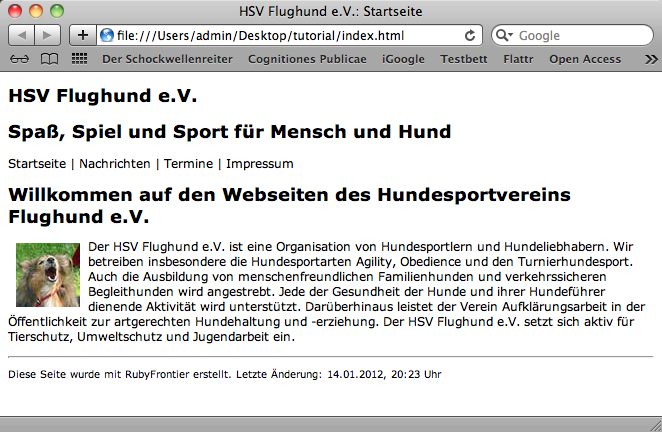
\includegraphics[width=0.7\textwidth]{./images/flughund03.png}
\caption{\label{flughund03}Screenshot 3: HSV Flughund e.V.}
\end{figure}

Das ist immer noch nicht wirklich weltbewegend, aber Sie ahnen sicher
schon, wohin die Reise gehen soll.


Die Navigation ist übrigens ein Dummy oder Mockup, wie es so schön auf
Neudeutsch heißt. Sie werden sie in einem späteren Abschnitt durch
eine funktionierende Navigation ersetzen, momentan dient sie aber erst
einmal als Platzhalter.


Sie ahnen sicher schon, daß die wesentlichen Änderungen, um ein
schönes Design zu bekommen, in der CSS-Datei geschehen müssen. Diese
ändern Sie daher wie folgt:


\begin{verbatim}
body {
    font-family: Verdana, sans-serif;
    font-size: 12px;
    background-color: #ffffcc;
}
h1 {
    font-size: 18px;
}
.small {
    font-size: 10px;
}
#header h1 {
    font-size: 32px;
}
#header h2 {
    font-size: 16px;
}
#navigation {
    background-color: #99cc99;
}
\end{verbatim}

Die ganze Seite bekommt nun wieder einen gelben Hintergrund (\#ffffcc),
die Überschriften im Header bekommen eine eigene Größe und die
Navigationsleiste eine lindgrüne (\#99cc99) Hintergrundfarbe
verpaßt. Nach einem erneuten Herausschreiben sollte Ihre Seite daher
nun so aussehen:

\begin{figure}[h!]
\centering
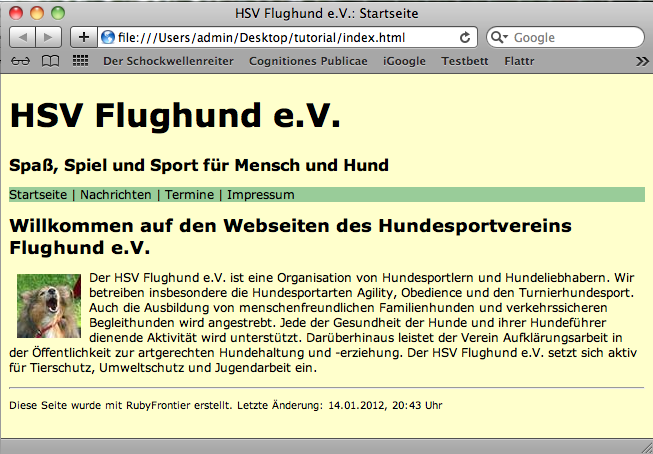
\includegraphics[width=0.7\textwidth]{./images/flughund04.png}
\caption{\label{flughund04}Screenshot 4: HSV Flughund e.V.}
\end{figure}


Und bitte vergessen Sie nicht, in der prefs.yaml die Zeile


\begin{verbatim}
:bgcolor: ffffff
\end{verbatim}

entweder komplett zu streichen oder auch hier den Wert ffffcc
einzusetzen. (Ich bin fürs streichen. Die Angabe der Hintergrundfarbe
und anderer Werte im body-Tag ist zwar sehr bequem und während der
Entwicklungsphase auch manchmal nützlich, aber eigentlich
überholt. Farben sollten nur noch in den Stylesheets festgelegt
werden. Wie Sie weiter unten sehen werden, kann die prefs.yaml dabei
aber dann doch wieder eine nützliche Rolle spielen.)


Ich erwarte übrigens nicht, daß Ihnen die Farben gefallen. Im
Gegenteil: Sie sind wieder aufgefordert, selber zu experimentieren und
andere Farben, Schriften und Größen auszuprobieren.


Abschließend möchte ich, daß Sie die Seite doch noch ein wenig
aufhübschen. Fast jede Website, die heutzutage etwas auf sich hält,
besitzt ein Hintergrundbild in der Kopfzeile, das etwas Stimmung
verbreitet und auf die Thematik der Seite hinweist. Dazu bringen Sie
erst einmal via Stylesheet die Seiten auf eine feste Breite von 920
Pixeln. Danach sieht die default.css wie folgt aus:


\begin{verbatim}
body {
    text-align: center; /* IE-Fix */
    font-family: Verdana, sans-serif;
    font-size: 12px;
    background-color: #ffffcc;
}
h1 {
    font-size: 18px;
}
.wrapper {
    width: 920px;
    margin: 0 auto;
    text-align: left; /* IE-Fix */
}
.small {
    font-size: 10px;
}
#header h1 {
    font-size: 32px;
}
#header h2 {
    font-size: 16px;
}
#navigation {
    background-color: #99cc99;
}
\end{verbatim}

Die beiden Ihnen vielleicht unverständlichen Zeilen mit den
Kommentaren IE-Fix dahinter sind eine Umgehung eines Fehlers des
Internet Explorers, der leider in vielen Fällen CSS nicht so
interpretiert, wie die Schöpfer es gewollt hatten. Ansonsten haben Sie
der Klasse wrapper die Breite von 920-Pixeln zugewiesen und mit auto
erreicht, daß diese 920 Pixel immer in der Mitte des Brwoserfensters
dargestellt wird.


Damit dieses Stylesheet funktioniert, schließen Sie im Template der
Seite den gesamten Inhalt in einen Wrapper ein:


\begin{verbatim}
<%= pageheader() %>
<div class="wrapper">
<div id="header">
    <h1>HSV Flughund e.V.</h1>
    <h2>Spaß, Spiel und Sport für Mensch und Hund</h2>
</div>
<div id="navigation">
    <p>Startseite | Nachrichten | Termine | Impressum</p>
</div>
<p id="bodytext"></p>
<hr />
<p class="small">Diese Seite wurde mit RubyFrontier erstellt.
Letzte Änderung: <%= clocknow() %></p>
</div>
<%= pagefooter() %>
\end{verbatim}

Wenn Sie alles richtig abgetippt haben, sollte nach einem erneuten
Herausrendern die Seite eine feste Breite besitzen und immer und die
Abstände rechts und links sollten immer gleich breit sein — egal,
wieweit Sie das Browserfenster aufziehen.

\begin{figure}[h!]
\centering
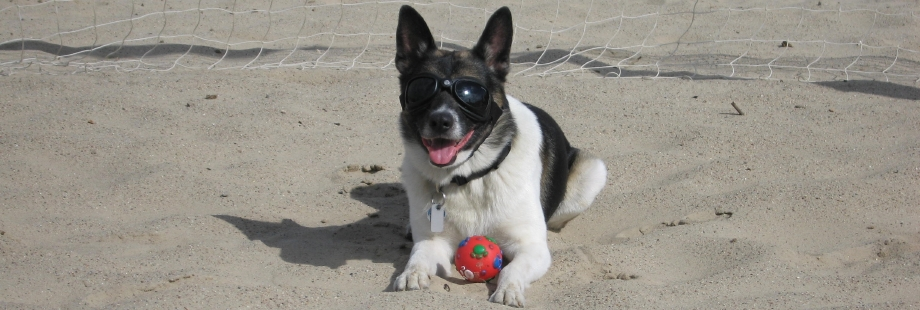
\includegraphics[width=0.7\textwidth]{./images/flughund-header.jpg}
\caption{\label{flughund-header}Header Image HSV Flughund e.V.}
\end{figure}


Das ist das Header-Bild, das ich für Sie ausgesucht habe. Laden Sie es
von der Webseite herunter, benennen Sie es in header.png um und legen
Sie es in den \#images-Ordner Ihres RubyFrontier-Projektes. Es ist im
Original 920 Pixel weit und 310 Pixel hoch. Sie können natürlich auch
ein anderes Bild wählen, Sie sollten es nur auf die gleichen
Abmessungen zuschneiden.


Da RubyFrontier seit der Version 0.9.9.6 Makros (aber keine
Direktiven!) auch in CSS- und JavaScript-Dateien erlaubt, sah mein
erster, naiver Versuch so aus:


\begin{verbatim}
#header {
    height: 310px;
    background-image: url(<%= imageref("header") %>);
    background-repeat: none;
}
\end{verbatim}

Sie können es ja selber ausprobieren. RubyFrontier schreibt Ihnen die
Seite anstandslos und ohne Fehlermeldung heraus, nur das gewünschte
Headerbild, das sehen Sie nicht. Wenn Sie sich den Quellcode des
herausgeschriebenen Stylesheets anschauen, sehen Sie, daß RubyFrontier
das Makro korrekt ausgewertet hat, aber auch, daß der relative Pfad
nicht vom Stylesheet, sondern von der index.txt aus berechnet
wurde. Das Verhalten ist ja eigentlich auch korrekt, wir haben ja die
index.txt herausgeschrieben. Matt Neuburg stellt in seiner
Frontier-Dokumentation unter anderem folgende Lösung vor:


In das Stylesheet fügen Sie bitte ganz oben auf der Seite (an erster
Stelle) folgendes Makro ein:


\begin{verbatim}
<% def writeAndGetRelativeURI(im)
       getImageData(im)[:path].relative_uri_from(adrPageTable[:sheetLoc])
end %>
\end{verbatim}

Sie sehen, dieses Makro hat kein Gleichheitszeichen nach dem <\%, das
bedeutet, es wird zwar ausgeführt, schreibt aber nichts in das
Stylesheet hinein, das somit valide bleibt.


Jetzt noch eine kleine Änderung im Style-Sheet …


\begin{verbatim}
#header {
    height: 310px;
    background-image: url(<%= writeAndGetRelativeURI("header") %>);
    background-repeat: none;
}
\end{verbatim}

und schon sehen Sie nach einem erneuten Herausschreiben das
Header-Bild auf der Seite:

\begin{figure}[h!]
\centering
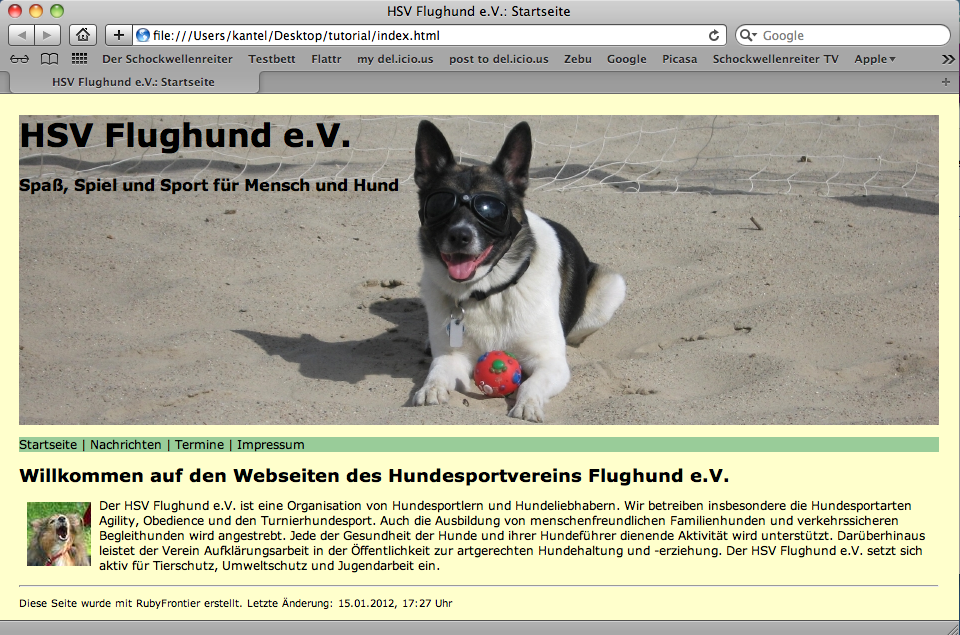
\includegraphics[width=0.7\textwidth]{./images/flughund05.png}
\caption{\label{flughund05}Screenshot 5: HSV Flughund e.V.}
\end{figure}

Okay, die Position des Vereinsnamens und des Untertitels sind noch
verbesserungswürdig, doch da dies eine Einführung in RubyFrontier und
nicht in CSS ist, schlage ich unkommentiert ein paar (einfache)
Änderungen im Stylesheet vor, die dies verschönert. Aber hier sind
auch Sie wieder aufgefordert, selber zu experimentieren und Ihre
CSS-Kenntnisse aufzufrischen (ich bin nämlich nicht gerade der große
CSS-Guru, eher im Gegenteil).


\begin{verbatim}
#header h1 {
    font-size: 32px;
    padding-left: 20px;
    padding-top: 200px;
    color: #ffffcc;
}
#header h2 {
    font-size: 16px;
    padding-left: 20px;
    color: #ffffcc;
}
\end{verbatim}

Ein linker Rand von 20 Pixeln und ein Abstand von 200 Pixel zum oberen
Rand machen das Ganze doch ein wenig ansehnlicher. Außerdem habe ich
den Überschriften die Farbe des Hintergrundes zugewiesen, so daß es
aussieht, als wären sie ausgestanzt.

\begin{figure}[h!]
\centering
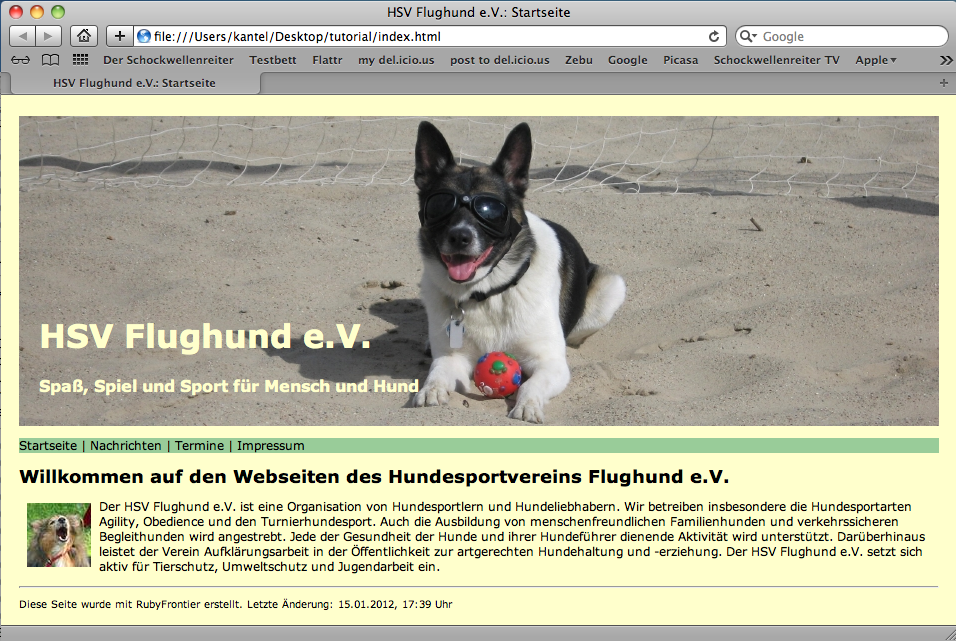
\includegraphics[width=0.7\textwidth]{./images/flughund06.png}
\caption{\label{flughund06}Screenshot 6: HSV Flughund e.V.}
\end{figure}

Die Website Ihres fiktiven Hundesportvereins nimmt nun langsam Gestalt
an: Zwar haben Sie immer noch erst eine Seite fertiggestellt, aber Sie
wissen jetzt, was ein Template ist und wie es Ihnen hilft, bei der
Seitengestaltung Form und Inhalt zu trennen. Außerdem wissen Sie nun,
wo Voreinstellungen festgelegt werden und wie RubyFrontier mit Bildern
und Stylesheets umgeht. Um nächsten Abschnitt werden Sie sich mit der
Navigation befassen und dabei weitere Vorzüge von RubyFrontier
kennenlernen.
\section{Navigare necesse est (Navigation tut Not)}
\label{sec-2-1-2}


In diesem Abschnitt werden Sie einen ersten Einblick in die
vielfältigen Möglichkeiten zur Website-internen Navigation, die
RubyFrontier bietet, bekommen.
\subsection{Neue Seiten aufziehen}
\label{sec-2-1-2-1}


\begin{figure}[h!]
\centering

\includegraphics[width 2cm]{./images/hund01.jpg}
\caption{\label{hund01}Zebu}
\end{figure}


Bevor Sie aber navigieren können, brauchen Sie natürlich einige Seiten
mehr in Ihrem Webauftritt. Und da nahezu jede Website heutzutage (in
Deutschland) ein Impressum benötigt, fangen Sie mit diesem an. Legen
Sie auf der gleichen Eben in Ihrem RubyFrontier-Projekt, in der Ihre
index.txt liegt, eine neue Seite an und nennen diese
impressum.txt. Außerdem laden Sie bitte das obenstehende Bildchen
eines Hundes herunter und legen dieses wie gewohnt in
den \#images-Ordner Ihres Projektes ab. Und dann schreiben Sie bitte
folgenden Text (oder etwas ähnliches) in die neuangelegte
impressum.txt-Datei:


\begin{verbatim}
#title "Impressum"

<h1><%= title %></h1>
<p>
Die nebenstehenden Informationen enthalten die gesetzlich vorgesehene
Anbieterkennzeichnung.</p>

<h4>Adresse</h4>
<p>
HSV Flughund e.V.<br />
Am Rollfeld 27<br />
12345 Hundesoßen</p>

<h4>Kontakt-Telephon</h4>

<table border="1" cellpadding="6" cellspacing="0">
    <tr>
        <th align="left">1. Vorsitzender</th>
        <td>Goofy Goldschatz</td>
        <td>011-111111</td>
    </tr>
    <tr>
        <th align="left">Welpengruppe</th>
        <td>Biby Bärchen</td>
        <td>022-222222</td>
    </tr>
    <tr>
        <th align="left">Kassenwart</th>
        <td>Pauly Panzer</td>
        <td>0$$-$$$$$$</td>
    </tr>
</table>
<p>
Zurück zur <a href="Startseite">Startseite</a>.</p>
<p>
<%= imageref("hund01") %></p>
\end{verbatim}

Das ist nicht gerade ein gesetzeskonformes Impressum, aber als
Beispiel reicht es. Und auch die Formatierung der Tabellen übernimmt
heutzutage in der Regel wieder ein Stylesheet, aber wie schon so
häufig wollte ich das Beispiel nicht unnötig aufblähen. Wenn Sie nun
diese Seite herausrendern, erhalten Sie dieses Bild:

\begin{figure}[h!]
\centering
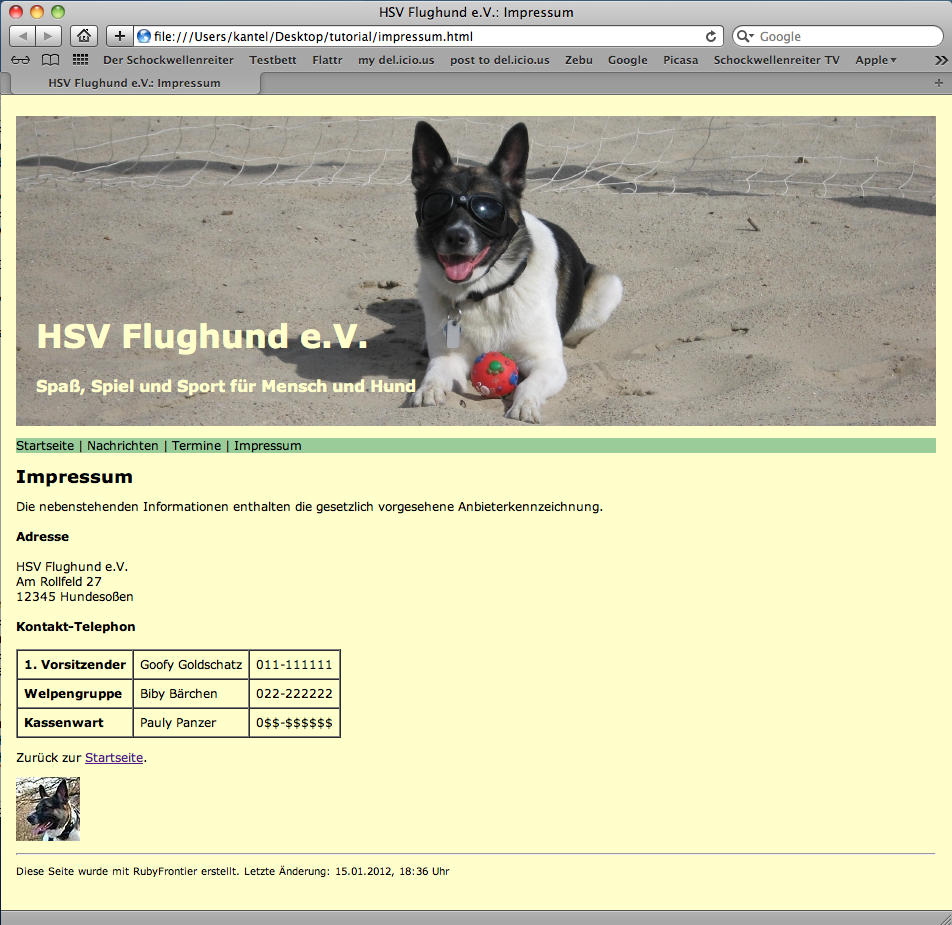
\includegraphics[width=0.7\textwidth]{./images/flughund07.png}
\caption{\label{flughund07}Screenshot 7: Impressum HSV Flughund e.V.}
\end{figure}


Es ist vermutlich genau das, was Sie erwartet haben: RubyFrontier hat
das Template genommen und es mit dem Text der Impressums-Seite
zusammengefügt. Nur da, wo Sie


\begin{verbatim}
Zurück zur <a href="Startseite">Startseite</a>.
\end{verbatim}

geschrieben haben, da erscheint tatsächlich ein Link. Und wenn Sie
darauf klicken, kommen Sie tatsächlich zurück zur Startseite
(vorausgesetzt, Sie haben sie auch herausgeschrieben). Dabei ist das,
nach allem was Sie und ich über HTML wissen, keine korrekte
Linkangabe. Was ist hier geschehen?


RubyFrontier verfügt, wie schon Frontier zuvor, über einen
Wiki-ähnlichen Mechanismus zur Linksubstitution. Für jede Seite, die
Sie in Ihrem RubyFrontier-Projekten anlegen, trägt es in
der \#autoglossary.yaml den Namen der Datei, den Titel und den Pfad
(die URL) zu dieser Datei ein. Wenn der Renderings-Mechanismus von
RubyForniter nun auf eine URL stößt, die nicht mit \href{http://}{http://} beginnt,
schaut er in dieser Datei nach, ob er einen passenden Eintrag dafür
findet. Wenn ja, ersetzt er dieses durch den passenden Link, wenn
nein, setzt er einen Link auf die (in der Regel nicht vorhandene)
Seite errorRefGlossaryFailedHere. So können Sie mit einer einfachen
Suche nach errorRefGlossaryFailedHere in der frisch generierten
HTML-Seite nach Fehlern suchen.


Sie können anstelle des Titels der Seite auch den Namen der Datei
(ohne Postfix), also in diesem Falle auch


\begin{verbatim}
Zurück zur <a href="index">Startseite</a>.
\end{verbatim}

eingeben, das funktioniert genau so. Aber nur, wenn tatsächlich auch
in allen Unterordnern der Name kein zweites Mal vorkommt, sonst gibt
es unter Umständen unerwünschte Seiteneffekte, denn RubyFrontier nimmt
den Eintrag, den es zuerst in der autoglossary.yaml findet, und das
gefundene Linkziel ist vielleicht nicht unbedingt das, auf das Sie
verlinken wollten. Daher hatte ich im letzten Abschnitt empfohlen, das
auch die Dateinamen innerhalb eines Projektes eindeutig sein
sollten. Aber auf jeden Fall sind Sie auf der sicheren Seite, wenn Sie
den Titel der Seite als Link verwenden, der muß eindeutig sein, sonst
steigt RubyFrontier mit einem Fehler aus.


Natürlich müssen Linkname und Link nicht übereinstimmen. Sie könnten
auch


\begin{verbatim}
Zurück zur <a href="Startseite">Heimatseite</a>
\end{verbatim}

schreiben, aber das haben Sie dann hoffentlich nur ironisch gemeint.
\subsection{Markdown: Es muß nicht immer HTML sein}
\label{sec-2-1-2-2}


Bei den beiden von Ihnen bsiher angelegten Seiten bestand der Inhalt
(bis auf ein paar Direktven und Makros) aus purem HTML. Nun stellen
Sie sich vor, Sie haben eine Seite, die häufig geändert werden muß,
weil sie zum Beispiel aktuelle Termine enthält. Dies in HTML zu
schreiben, kann ganz schön umständlich sein, wie schnell hat man da
mal einen Tag vergessen und schon haut es einem die Seite kaputt.


Es gibt dazu jedoch in RubyFrontier (mindestens) eine Alternative, die
schon mehrfach erwähnte Auszeichnungssprache Markdown. Sie will kein
Ersatz für HTML sein, sondern etwas, das den Schreibenden unterstützt,
schnell zu schreiben, ohne sich viel um die Formatierungen kümmern zu
müssen. Schauen Sie sich das einfach an einem Beispiel an, mehr zu
Markdown gibt es in einem separaten Kapitel.


Dazu legen Sie eine weitere Seite in der gleichen Ebene wie die
index.txt und die impressum.txt an und nennen Sie diese
termine.txt. Dort schreiben Sie bitte folgenden Text hinein:


\begin{verbatim}
#title "Termine"
#markdown "True"

# <%= title %>

#### 12. Februar 2012

Agility-Winterturnier in der Reithalle an der Pferdestraße in Altenhunden.
Beginn 9:00 Uhr, die Meldestelle öffnet um 8:00 Uhr.

#### 21. Februar 2012

Gemeinsames Obedience-Training mit den Sportsfreunden vom HSV Doppelhunden
auf unserem Platz. Beginn 10:00 Uhr. **Bitte die Hunde nicht vergessen!**

Um 9:00 Uhr gibt es ein gemeinsames Frühstück. Wer daran teilnehmen möchte,
melde sich bitte wegen der Einkaufsplanung bei *Biby*.

#### 29. Februar 2012

Mitgliederversammlung. Beginn 19:00 Uhr im Vereinsheim. Bitte
Mitgliedsausweise mitbringen.

----

zurück zur [Startseite](Startseite)
\end{verbatim}

Auch wenn Sie jetzt von mir denken »Der Kerl ist wahnsinnig, was soll
denn das?«, rendern sie die Seite doch einfach heraus. Sie sollte so
aussehen:

\begin{figure}[h!]
\centering
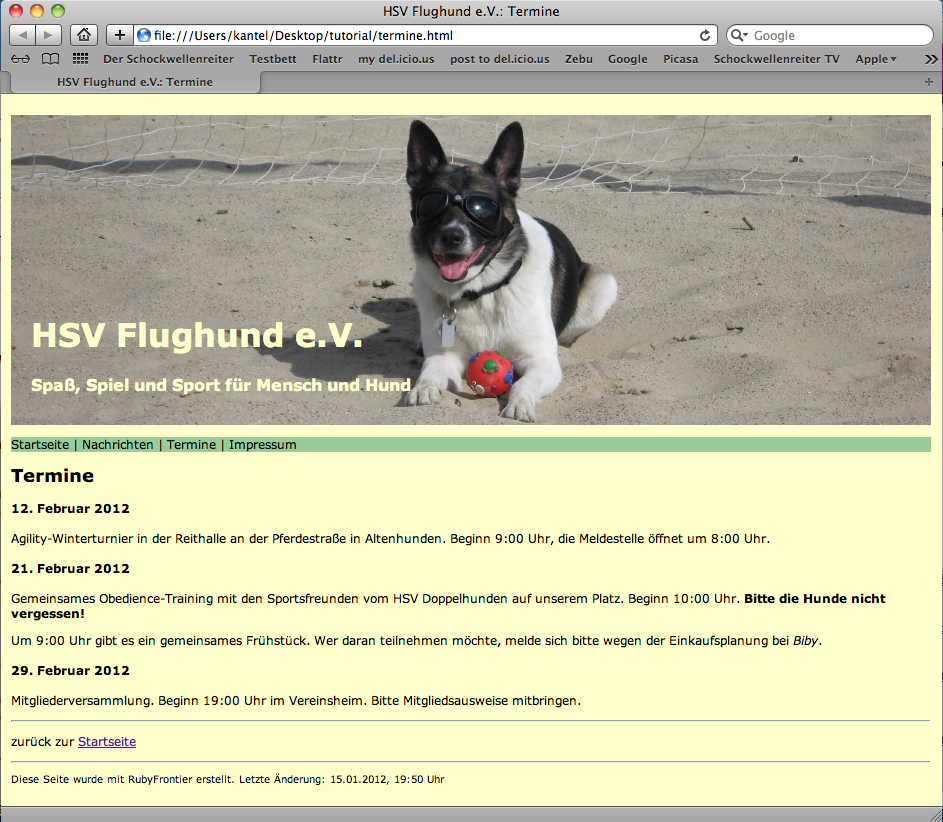
\includegraphics[width=0.7\textwidth]{./images/flughund08.png}
\caption{\label{flughund08}Screenshot 8: Termine HSV Flughund e.V.}
\end{figure}


Schauen Sie sich das Ergebnis in Ruhe an. Die erste Zeile legt wie
gewohnt den Titel fest. Dann folgt eine weitere Direktive, die
RubyFrontier mitteilt, daß diese Seite mit Markdown erstellt
wurde. Danach werden Sie freudig festellten, daß Direktiven (und auch
Makros) mit Markdown ebenfalls funktionieren und genau so wie in
HTML-Seiten geschrieben werden. Ein Doppelkreuz (\#) am Anfang einer
Zeile kennzeichnet eine h1-Überschrift, zwei somit eine h2-Überschrift
und wo weiter …


Absätze werden durch zweimaliges Drücken der Return-Taste erzeugt,
Fetter Text ist mit zwei Sternchen umsäumt, kursiver Text mit einem
Stern. Und vier Striche in einer Reihe erzeugen eine waagrechte Linie.


Links werden in Markdown so notiert


\begin{verbatim}
[Linktext](URL)
\end{verbatim}

und Sie haben sicher mit Freuden schon festgestellt, daß die
Glossary-Substitution


\begin{verbatim}
[Startseite](Startseite)
\end{verbatim}

von RubyFrontier auch hier funktioniert. (Das ist überhaupt der Grund,
warum ich die ersten Schritte mit Markdown hier in dem Abschnitt über
Navigation aufgenommen habe.)


Markdown bietet noch viele Möglichkeiten und auch Alternativen zur
Auszeichnung. Die im obigen Text benutzten sind die, die am häufigsten
und fast ausschließlich von mir verwendet werden. Markdown kann noch
ein wenig mehr und das, was es nicht kann, können Sie erreichen, indem
Sie einfach HTML-Tags an diesen Stellen schreiben.
\subsection{Unsere letzte Seite}
\label{sec-2-1-2-3}


Bevor Sie sich aber endgültig der Navigation zuwenden, legen Sie bitte
noch eine letzte Seite an, die Sie nachrichten.txt nennen.

\begin{figure}[h!]
\centering
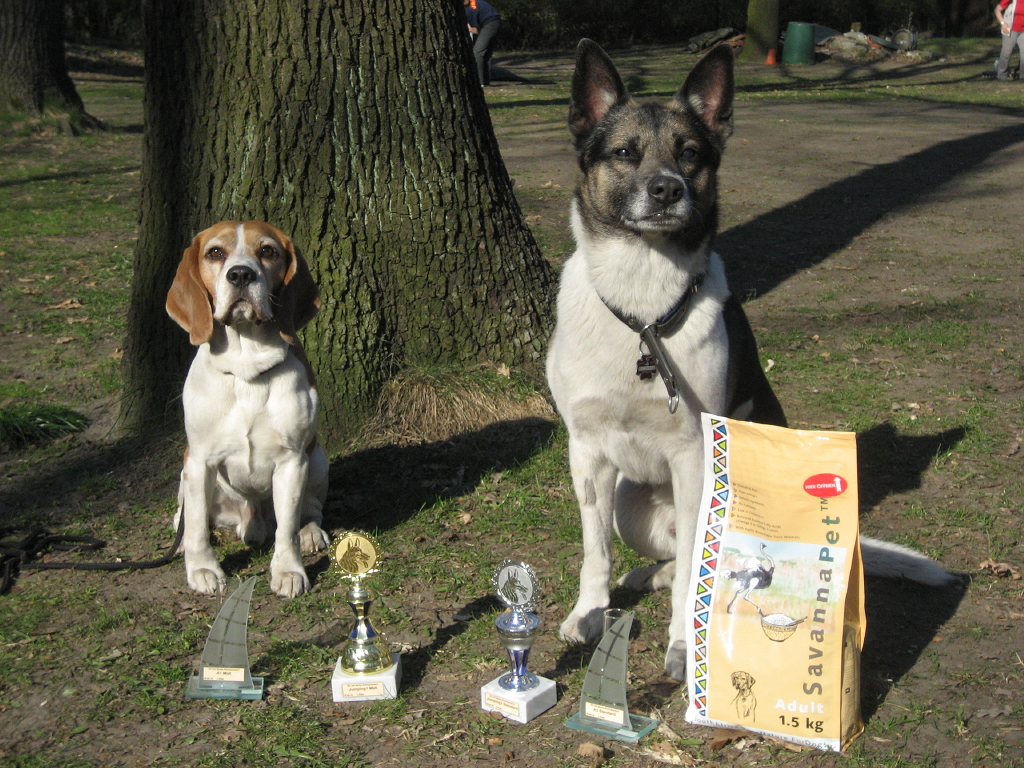
\includegraphics[width=0.7\textwidth]{./images/sieger.jpg}
\caption{\label{sieger}So sehen Sieger aus!}
\end{figure}

\begin{itemize}
\item So sehen Sieger aus!
\end{itemize}

Wenn sie genau so aussehen soll, wie dieses Tutorial laden Sie bitte
erst einmal das obige Bild herunter (es heißt sieger.jpg) und packen
es wie gewohnt in den \#images-Ordner Ihres Projektes.

Dann schreiben Sie bitte folgenden Text in diese Seite:


\begin{verbatim}
#title "Nachrichten"
#markdown "True"

# Nachrichten aus dem Vereinsleben

## Zebu und der Bollerbeagle auf dem Siegertreppchen

<%= imageref("sieger", {:border => "0", :width => "480", :height => "360",
:alt => "So sehen Sieger aus!"}) %>

Auf dem ersten Agility-Turnier dieses Jahres bei den Sportsfreunden in
Altenhunden räumten der Bollerbeagle mit Frau Chen und Zebu mit Herr Chen
gewaltig ab und gewannen sowohl den A-Lauf wie auch den Jumping. Zebu
wurde außerdem Tagessieger und bekam zur Belohnung eine große Tüte Hundefutter.
Wir gratulieren!

## Bilder von der Weihnachtsfeier

Die bestellten Bilder von der Weihnachtsfeier sind eingetroffen. Sie können
gegen Bezahlung bei Biby während der Trainingszeiten im Vereinsheim abgeholt
werden.
\end{verbatim}

Wenn Ihnen der Text zu dämlich ist, können Sie natürlich
hineinschreiben, was Sie wollen. Wichtig ist nur, daß die ersten
beiden Zeilen mit den Direktiven unangetastet bleiben.

Wie Sie sehen, habe ich auch hier wieder Markdown als
Auszeichnungssprache verwendet. Es macht einem vieles einfacher.

Die Seite besitzt zwei Überschriften 2. Ordnung. Wenn Sie sich noch an
das Stylesheet erinnern, haben Sie dafür noch keinen Stil
angelegt. Das holen Sie daher bitte jetzt nach und schreiben in die
default.css an passender Stelle (wo, ist eigentlich egal, ich habe es
direkt hinter die h1-Definition geschrieben):


\begin{verbatim}
h2 {
    font-size: 16px;
}
\end{verbatim}

Wenn Sie die Seite jetzt herausschreiben, sollte sie so aussehen:

\begin{figure}[h!]
\centering
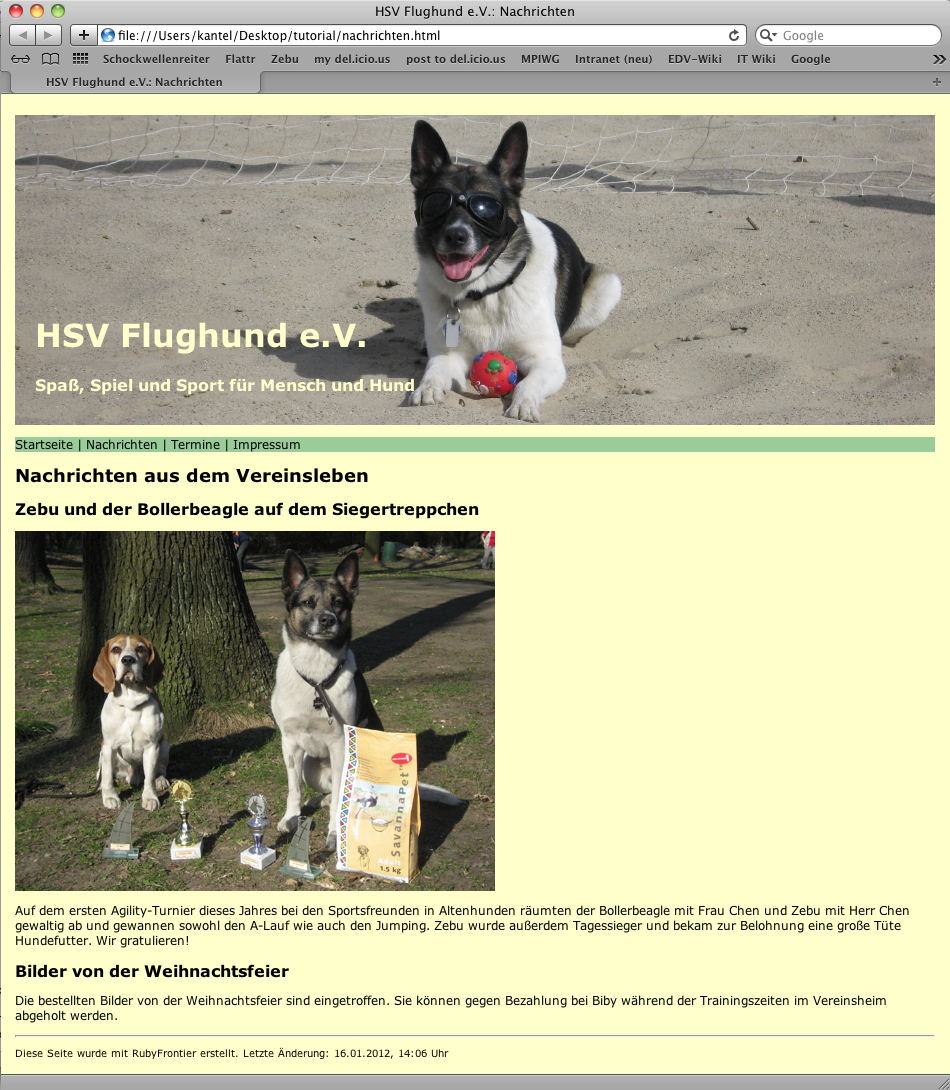
\includegraphics[width=0.7\textwidth]{./images/flughund09.png}
\caption{\label{flughund09}Screenshot 9: Nachrichten HSV Flughund e.V.}
\end{figure}
\subsection{Aber jetzt: Navigation!}
\label{sec-2-1-2-4}


Sie haben sicher gut aufgepaßt und so ist Ihnen aufgefallen, daß nun
genau die Seiten, die ich anfangs in die Dummy-Navigation des
Templates geschrieben habe, erstellt wurden. Und die möchte ich nun
gemeinsam mit Ihnen mit den entsprechenden Links versehen.


Um dies zu erreichen, gibt es einen sehr einfachen Weg: Sie schreiben
einfach die Links in das Template. Öffnen Sie es in TextMate und
ändern die Zeilen


\begin{verbatim}
<div id="navigation">
    <p>Startseite | Nachrichten | Termine | Impressum</p>
</div>
in

<div id="navigation">
    <p><a href="Startseite">Startseite</a> | <a href="Nachrichten">
    Nachrichten</a> | <a href="Termine">Termine</a> | <a href="Impressum">
    Impressum</a></p>
</div>
\end{verbatim}

(Wie schon in einigen Beispielen zuvor wurden die Zeilenumbrüche nur
der besseren Lesbarkeit wegen hinzugefügt.)

Wenn Sie jetzt mit Publish Site alle Seiten herausrendern, werden Sie
merken, daß RubyFrontier sehr schlau ist und mitdenkt: In der
lindgrünen Linkleiste sind alle Seiten mit Links versehen, nur die
gerade aktuelle, auf der Sie sich befinden, nicht. Das heißt, die
Seite linkt nicht auf sich selber. Wer so etwas schon einmal von Hand
basteln mußte, wird der Software sicher sehr dankbar sein. Das ist ein
weiterer Vorteil des Glossary-Mechanismus, der genau dies für Sie
erledigt hat.

Als letzten Akt wollte ich der Navigation noch etwas Raum zum Atmen
geben und habe daher an das Ende der default.css noch diese Zeilen
angefügt:


\begin{verbatim}
#navigation p {
    padding-left: 10px;
    padding-top: 5px;
    padding-bottom: 5px;
}
\end{verbatim}

Wenn Sie jetzt noch einmal mit Publish Site alle Seiten
herausschreiben, sehen Sie das endgültige Ergebnis Ihrer Bemühungen:


\begin{figure}[h!]
\centering
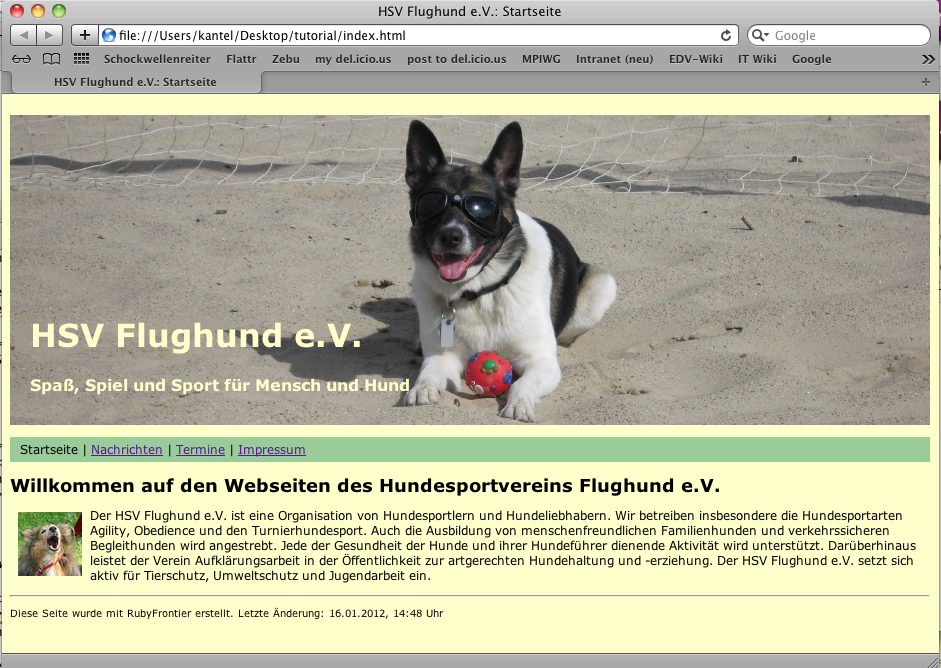
\includegraphics[width=0.7\textwidth]{./images/flughund10.png}
\caption{\label{flughund10}Screenshot 10: Wir haben fertig!}
\end{figure}


Gratuliere! Sie haben Ihre erste vollständige Website mithilfe von
RubyFrontier erstellt. Es ist eine einfache Website, aber wenn Sie
sich etliche Webauftritte von Kleinunternehmen, Selbstständigen oder
eben auch Vereinen anschauen, dann ist es genau das, was gewünscht
wird. Dabei haben Sie bisher nur an der Oberfläche von RubyFrontier
gekratzt. Daß Sie trotzdem schon so weit gekommen sind, spricht für
RubyFrontier. In den nächsten Kapiteln werden wir sukkzessive weiter
in die Tiefe gehen und etliches von den erweiterten Möglichkeiten
RubyFrontiers kennenlernen.


Aber natürlich sollen Sie auch hier nicht stehenbleiben. Spielen Sie
mit Ihrer erstellten Site herum, experimentieren Sie mit den Farben
(sicher werden Sie zu dem Ergebnis kommen, daß ein weißer Hintergrund
vielleicht doch schöner ist) und dem anderen Gelernten, fügen Sie
weitere Seiten hinzu etc. Und wenn Sie dabei das Gefühl entwickeln
»RubyFrontier macht Spaß!«, dann sind Sie auf jeden Fall bereit für
die nächsten Kapitel.
\chapter{Exkurs: RubyFrontier und MAMP}
\label{sec-2-2}


\begin{figure}[h!]
\centering
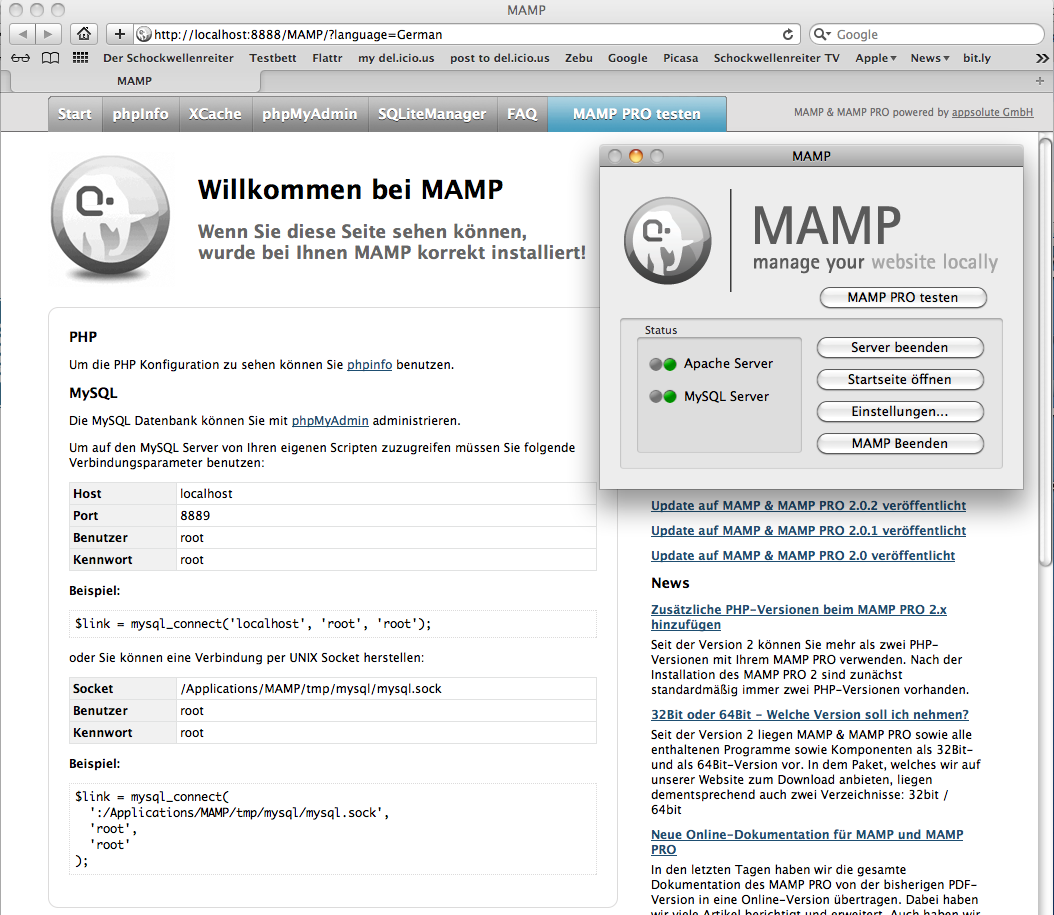
\includegraphics[width=0.7\textwidth]{./images/mamp01.png}
\caption{\label{mamp01}MAMP-Kontrollcenter und MAMP-Startseite}
\end{figure}
\section{Was ist MAMP?}
\label{sec-2-2-1}


Die Abkürzung »MAMP« steht für Macintosh, Apache, Mysql und PHP. Es
ist eine Umgebung, die Ihnen mit wenigen Mausklicks eine
Serverumgebung für Testzwecke zur Verfügung stellt. Das kann für die
Arbeit mit RubyFrontier recht nützlich sein. Denn statische Seiten hin
oder her, manchmal benötigen Sie doch dynamische Elemente oder
Datenbankzugriffe für Teile Ihrer Website — und sei es nur für ein
Kontaktformular.

Aber auch als Entwicklungs- und Testumgebung für AJAX-Anwendungen ist
die Kombination RubyFrontier/MAMP ein sehr nützliches und komfortables
Paket. Beachten Sie jedoch eines: MAMP wurde als Entwicklungsumgebung
für den Desktop konzipert, es sollte aus Sicherheitsgründen niemals
als Produktionsumgebung eingesetzt werden.

MAMP installiert sich per Default im Programme-Ordner Ihres Macs und
alles, was MAMP benötigt, liegt innerhalb dieses Ordners. Es fummelt
also nicht im »normalen« Betriebssystem herum. Und wenn Sie MAMP nicht
mehr benötigen oder sich total verkonfiguriert haben — schieben Sie
einfach den kompletten MAMP-Ordner in den Papierkorb und schon haben
Sie wieder einen sauberen Mac. Und dann laden Sie einfach eine neue
MAMP-Umgebung von der Website des Herstellers herunter und mit wenigen
Klicks besitzen Sie eine neue Umgebung.

Der Vorteil kann unschätzbar sein. Ich habe zum Beispiel einmal den
(eingebauten) Webserver des OPML Editors auf einer meiner Maschinen so
verkonfiguriert, daß sich der zum MacOS X gehörende interne Apache
nicht mehr starten ließ. Ich hatte Stunden gebraucht, um dies wieder
zu beheben. Das kann Ihnen mit MAMP nicht passieren.

Und während Frontier (und zumindest zeitweise auch der OPML Editor)
ein Webserver auf dem Desktop ist, der auch statische Seiten
herausschreiben kann, ist die Kombination RubyFrontier/MAMP ein Tool,
das statische Seiten herausschreibt, aber auch als Webserver auf dem
Desktop funktioniert. Damit kann man im Prinzip all das anstellen, was
Winer und andere mit dem OPML Editor anstellen. Man muß sich
allerdings an die Skriptsprache PHP gewöhnen. Aber die ist eigentlich
recht einfach zu erlernen und da die Anwendung ja nur auf dem Desktop
läuft, müssen Sie sich auch nicht mit Sicherheitsanforderungen, die
die Programmierung von PHP-Anwednugen oft verkompliziert,
herumschlagen.

MAMP ist Open Source und steht unter der GPL, das heißt, Sie können
die Software kostenlos herunterladen und nutzen. Und lassen Sie sich
nicht beirren. Auf der Website wird versucht, Sie ständig auf das
kostenpflichtige MAMP PRO zu locken. Zumindest für das, was Sie hier
in diesem Tutorial anstellen — und vieles, vieles mehr —, brauchen Sie
MAMP PRO nicht. Das kostenlose MAMP genügt völlig.

(Professionelle Webentwickler — vielleicht gibt es ja auch unter den
Lesern dieses Tutorials einige — dürfen aber ruhig einmal einen Blick
auf MAMP PRO werfen. Der wichtigste Unterschied ist, daß die Server
über Dienste wie z.B. DynDNS auch nach außen sichtbar gemacht werden
können. Auch MAMP PRO sollte nicht für Produktionszwecke eingesetzt
werden, aber um einen entfernt sitzenden Kunden die neuesten
Entwicklungen eines Projektes zu zeigen oder um Tests mit den
Anwendern beim Kunden durchzuführen, kann sich die Anschaffung von
MAMP PRO durchaus lohnen. Denn die Alternativen wären die Installation
eines Testsystems entwender beim Kunden oder bei einem externen
Provider.)
\section{Installation und Konfiguration}
\label{sec-2-2-2}


Die Installation von MAMP ist wirklich einfach. Sie gehen auf die
Webseite des Herstellers und laden Sie MAMP (nicht MAMP PRO)
herunter. Und erschrecken Sie sich nicht. Aktuell ist das Paket 116 MB
schwer und bringt auch eine Testversion von MAMP PRO mit. Ein
Doppelklick auf die heruntergeladene Datei MAMP.pkg startet die
Installation. Wenn Sie nicht genau wissen, was Sie vorhaben, belassen
Sie es bei den Voreinstellungen, die der Installer Ihnen
vorschlägt. Sie haben sich bei mir bewährt. Nach der Installation
haben Sie einen Ordner MAMP und einen Ordner MAMP PRO in dem
anwenderübergreifenden Programme-Ordner Ihres Macs. Innerhalb des
Ordners MAMP finden Sie das Programm MAMP. Es empfiehlt sich, um
schnelleren Zugriff zu haben, dieses im Dock abzulegen.


Nach dem ersten Start öffnet sich eine Webseite und ein kleines
Dialogfenster, das MAMP-Kontrollcenter genannt wird. Mit einem Klick
auf Einstellungen können Sie einige Einstellungen vornehmen:

\begin{figure}[h!]
\centering
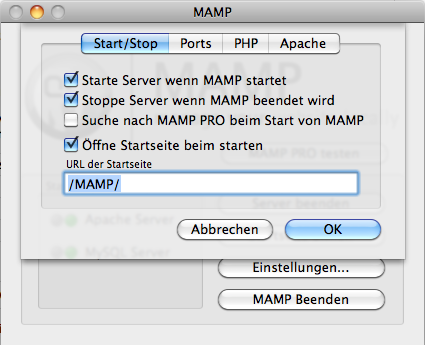
\includegraphics[width=0.7\textwidth]{./images/mamp02.png}
\caption{\label{mamp02}MAMP-Kontrollcenter}
\end{figure}


Als erstes klicke ich immer »Suche nach MAMP PRO beim Start von MAMP«
weg. Danach können Sie nämlich den Ordner MAMP PRO bedenkenlos in den
Papierkorb schieben, ohne daß es eine Fehlermeldung gibt. In dem
Reiter Start/Stop lohnt es sich, Ihr gerade aktuelles Projekt
einzutragen. Dies erspart Ihnen sehr viel Zeit. Ich komme später
darauf zurück.

\begin{figure}[h!]
\centering
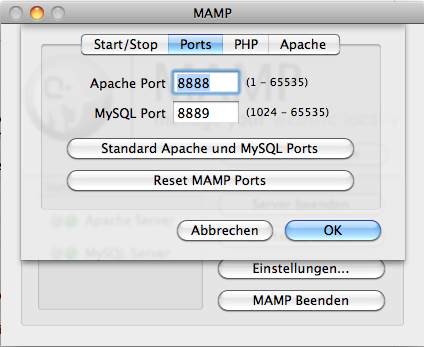
\includegraphics[width=0.7\textwidth]{./images/mamp03.png}
\caption{\label{mamp03}MAMP-Kontrollcenter: Ports}
\end{figure}

Die übrigen Einstellungen können Sie erst einmal so belassen, sie sind
sowieso eher etwas für Spezialisten. Überprüfen Sie lediglich die
Ports, wenn Sie andere Anwendungen auf Ihrem Rechner betreiben, die
bereits Ports belegen. Per Default lauscht MAMPs Apache auf Port 8888
und das dazugehörende MySQL auf Port 8889.
\subsection{RubyFrontier mit MAMP testen}
\label{sec-2-2-2-1}


Um RubyFrontier mit MAMP zu testen, müssen Sie als erstes festlegen,
daß RubyFrontier die Dateien dahin schreibt, wo MAMP sie auch lesen
kann. Wenn Sie sich die Ordnerstruktur innerhalb des MAMP-Ordners
angeschaut haben, werden Sie dort den Ordner htdocs gesehen
haben. Dies ist der Ordner, in dem der Apache des MAMP seine Dateien
erwartet und sie ausliest. Und Sie erinnern sich sicher, daß wir
bisher die Dateien auf den Schreibtisch Ihres Macs herausgeschrieben
haben. Um das zu ändern, öffnen Sie die Datei ftpSite.yaml und ändern
den Eintrag :folder wie folgt:


\begin{verbatim}
:folder: /Applications/MAMP/htdocs/tutorial
\end{verbatim}

Falls Sie Ihre MAMP-Installation irgendwo anders abgelegt haben,
müssen Sie diese Zeile natürlich anpassen.


Jetzt rendern Sie am Besten alle Ihre Tutorial-Seiten noch einmal
heraus. Danach sollten Sie im Ordner htdocs ein Unterordner tutorial
finden. Wenn Sie jetzt Ihren Browser nach
\href{http://localhost:8888/tutorial/}{http://localhost:8888/tutorial/} schicken, sollten Sie die Startseite
des Hundesportvereins sehen können. (Den Ordner tutorial auf Ihrem
Desktop können Sie nun in den Papierkorb schieben, er wird nicht mehr
gebraucht.)


Etwas unangenehm ist natürlich, daß RubyFrontier Ihren
Standard-Browser ebenfalls anweist, die Seite zu öffnen und zwar
unter:


\begin{verbatim}
file:///Applications/MAMP/htdocs/tutorial/index.html
\end{verbatim}

Daher ist noch etwas zu tun. Denn Matt Neuburg hat diesen Fall
natürlich vorausgesehen und Abhilfe geschaffen. Öffnen Sie die
Datei \#ftpSite.yaml und fügen Sie folgende zwei Zeilen darin ein:


\begin{verbatim}
:apacheSite: /Applications/MAMP/htdocs/tutorial
:apacheURL: http://localhost:8888/tutorial/
\end{verbatim}

Wenn dieser Eintrag vorhanden ist, öffnet RubyFrontier alle
HTML-Seiten via HTTP unter der angegeben URL.


Jetzt wollen Sie natürlich endlich eine Testseite schreiben. Legen Sie
also eine neue Seite an, die sie phptest.txt nennen und schreiben Sie
folgendes hinein:


\begin{verbatim}
#title "PHP-Test"
#fileextension ".php"

<h1>Hallo PHP!</h1>

<?php
    print "<p>Hallo PHP-Welt. Dieser Text wird von PHP herausgeschrieben.</p>
    <p>Das ist doch einfach, oder?</p><br /><br />"
?>
\end{verbatim}

fileextension ist eine Direktive, die die Dateiendung festlegt. Der
Default ist natürlich .html, aber da der Apache nur erkennt, wann er
eine Datei zum PHP-Interpreter weiterleiten soll, wenn diese die
Dateiendung .php besitzt, müssen Sie dieses natürlich RubyFrontier
mitteilen. (Wenn Sie sich mit der Konfiguration des Apache auskennen,
wissen Sie natürlich, daß man dieses auch ändern kann, aber ich möchte
doch beim Standardverhalten bleiben.)


Ein PHP-Skript steht (fast) immer zwischen


\begin{verbatim}
<?php
    *Ihr eigener Code hier*
?>
\end{verbatim}

Es gibt zwar Alternativen, aber auch dies hat sich als Standard
etabliert und Sie sollten nur davon abweichen, wenn Sie genau wissen,
was Sie tun. Rendern Sie die Seite heraus. Als erstes werden Sie
feststellen, daß dieses mal RubyFrontier kein Browserfenster
automatisch öffnet, da die Software schlau genug ist, um zu wissen,
daß bei einer Änderung des Dateiendes nicht unbedingt eine HTML-Datei
herausgeschrieben wird, die man sich im Browser anschauen möchte. Also
schicken Sie Ihren Browser zu
\href{http://localhost:8888/tutorial/phptest.php}{http://localhost:8888/tutorial/phptest.php} und voila …

\begin{figure}[h!]
\centering
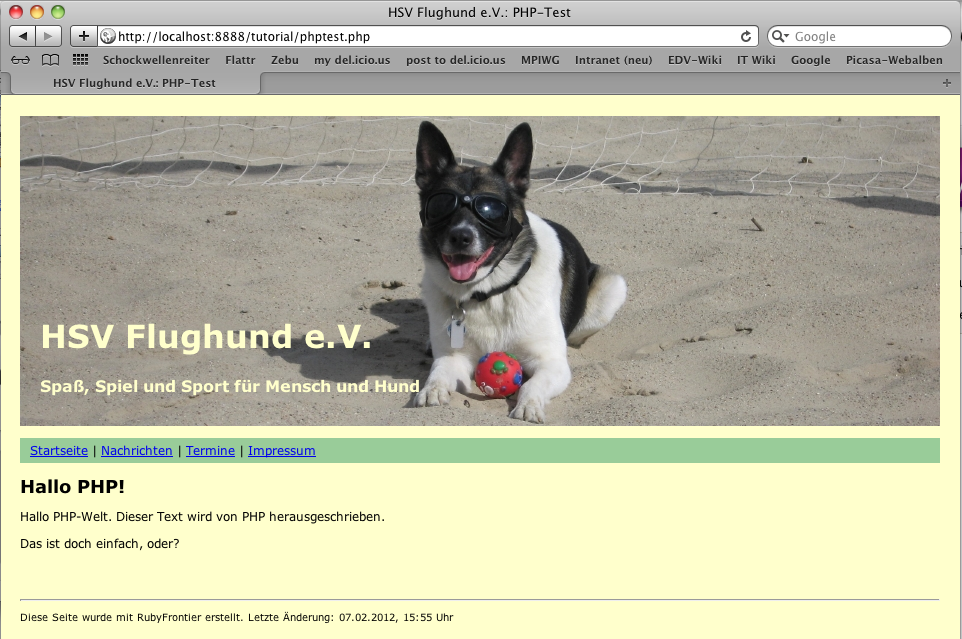
\includegraphics[width=0.7\textwidth]{./images/phptest01.png}
\caption{\label{phptest01}Ihre erste PHP-Seite}
\end{figure}


Gratuliere, Sie haben erfolgreich Ihr erstes PHP-Skript geschrieben.

Zum Schluß können Sie sich die Sache noch ein wenig komfortabler
gestalten. Wenn Sie in den MAMP-Einstellungen den Ordner Ihres
aktuellen Projektes eintragen, also — wenn Sie alles so angelegt
haben, wie hier beschrieben —

\begin{figure}[h!]
\centering
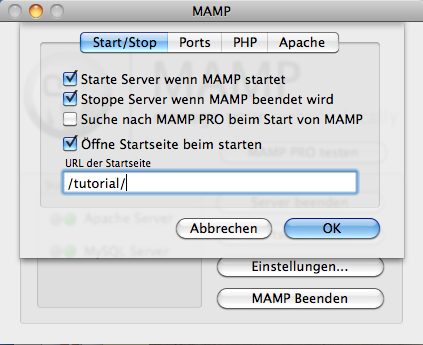
\includegraphics[width=0.7\textwidth]{./images/mamp04.png}
\caption{\label{mamp04}Die MAMP-Startseite ändern}
\end{figure}


den Ordner \emph{tutorial}, dann öffnet MAMP beim Start die Index-Seite
dieses Projekts. Für den Fall, daß Sie die werksseitigen Startseiten
wieder benötigen (z.B. um an den PHP- oder Datenbankeinstellungen zu
schrauben), sollten Sie sich jedoch merken, daß diese im Verzeichnis
\emph{MAMP} liegen und dieses bei Bedarf auch wieder eintragen.


Doch MAMP ist nicht nur nützlich, um PHP-Skripte zu erstellen. Um der
Wahrheit die Ehre zu geben: Ich selber skripte sehr, sehr selten in
PHP. Aber auch einige JavaScripte erwarten, daß sie hinter einem
Apache oder ähnlichem Webserver laufen, speziell die Skripte, die
»nach Hause telephonieren«. Schauen Sie zum Beispiel mal auf dieses
Stück JavaScript (der Zeilenumbruch dient nur der besseren
Lesbarkeit):


\begin{verbatim}
<script type="text/javascript"><!-- 
amazon_ad_tag = "derschockwell-21"; amazon_ad_width = "468";
amazon_ad_height = "60"; amazon_ad_logo = "hide";
amazon_ad_discount = "remove";//--></script>
<script type="text/javascript" src="http://www.assoc-amazon.de/s/ads.js">
</script>
\end{verbatim}

Es ist ein Script, daß Amazons JavaScript API nutzt, um für den Inhalt
der Seite passende Werbung herauszusuchen. Dafür muß es natürlich den
Text der Seite nach Amazon schicken. Wenn Sie testweise dieses Skript
in eine Seite einbauen und diese dann via \href{file:///}{file:///} aufrufen, sehen Sie
nichts. Läuft die Seite aber hinter einem MAMP und wird via HTTP
aufgerufen, erscheint die Anzeige in ihrer ganzen Schönheit:

\begin{figure}[h!]
\centering

\includegraphics[width=0.7\textwidth]{./images/amazon.png}
\caption{\label{amazon}Amazon-Werbung}
\end{figure}

Auch wenn Sie keine Werbung für Amazon auf Ihren Webseiten machen
wollen, es gibt etliche andere JavaScript APIs, die sich ähnlich
verhalten, so einige der APIs von Google, unter anderem für Google
Maps. Und gerade für Webmapping-Anwendungen wird auch die Kombination
JavaScript auf der Client-Seite und PHP auf dem Server wieder
interessant.


Sie sehen also, es kann durchaus wichtige Gründe geben, sich MAMP
zusammen mit RubyFrontier zu installieren.
\section{RubyFrontier, MAMP und die Tropfenschachtel}
\label{sec-2-2-3}


Es gibt keine Vorschrift, daß MAMP — wie alle anderen
Macintosh-Programme auch — im Ordner »Programme« abgelegt sein muß. Es
hindert Sie nichts daran, MAMP im Dropbox-Ordner zu
installieren. Allerdings sollten dann alle ihre damit verbundenen
Rechner über einen sehr schnellen Internet-Anschluß verfügen, da je
nachdem wie intensiv sie mit MAMP arbeiten, schon sehr viele Daten
hin- und hergeschaufelt werden können.


Außer bei sehr großen Projekten sehe ich auch keinen Vorteil
darin. Daher habe ich stattdessen MAMP auf allen angeschlossenen
Rechner installiert und synchroniere lediglich die Quelldateien (im
Projekt-Ordner) über die Dropbox. Das hängt aber auch damit zusammen,
daß ich etliche andere, zum Teil sehr große Projekte zumindest im
Entwicklungsstadium mit MAMP bearbeite und ich mir so die
Tropfenschachtel ziemlich »vollmüllen« wurde. Probieren Sie daher
selber aus, ob dieses Vorgehen für Sie geeignet ist.
\chapter{Exkurs: RubyFrontier und die Dropbox}
\label{sec-2-3}
\chapter{Eine Bildergalerie mit RubyFrontier}
\label{sec-2-4}


Natürlich gehört zu jeder guten Vereinswebseite auch eine
Photogalerie. Diese werden Sie daher als nächstes anlegen. Dabei
lernen Sie dann auch einige neue Features von RubyFrontier kennen,
beispielsweise den Vererbungsmechanismus von RubyFrontier oder wie Sie
mit alternativen Templates umgehen. Aber auch, wie Sie Bilder nicht
nur lokal, sondern auch von Webdiensten wie flickr oder dem Picasa Web
Album von Google in Ihren Seiten einbinden können.


Da die Seiten ja nur ein Beispiel sind und um den Aufwand erträglich
zu halten, wird jede Galerie nur aus vier Photos bestehen. Laden Sie
daher zu Beginn diese vier Photos meines Hundes Zebu (einem
Schäferhund-Husky-Mix) herunter.

\begin{figure}[h!]
\centering
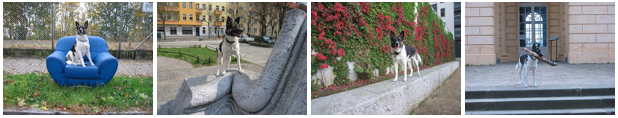
\includegraphics[width=0.7\textwidth]{./images/hundebilder01.png}
\caption{\label{hundebilder01}Hundebilder Zebu}
\end{figure}


Es ist der Hund, der auch die Titelleiste der Seiten Ihres (oder
unseres) fiktiven Hundesportvereins ziert. Die Sonnenbrille, die er
dort trägt, war keine Spinnerei, sondern der Hund litt an einer
Überempfindlichkeit gegenüber UV-Licht und trug daher eine Brille, die
in der Schweiz zum Schutz der Augen von Lawinenhunden entwickelt
worden war.


Zebu starb leider im Dezember 2010 an Krebs. Er wurde nur neun Jahre
jung. Mein zweiter Hund war dann ein Sheltie mit dem Zwingernamen Joey
vom Zillegarten, ein kleiner Hütehund von den Shetland-Inseln. Auch
von ihm habe ich vier Bilder ausgesucht, die Sie bitte herunterladen.

\begin{figure}[h!]
\centering
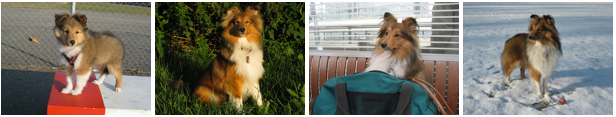
\includegraphics[width=0.7\textwidth]{./images/hundebilder02.png}
\caption{\label{hundebilder02}Hundebilder Joey}
\end{figure}

Die Bilder habe alle eine Größe von 500 mal 375 Pixeln, damit die
Galerie einheitlich aussieht. Aber natürlich steht es Ihnen — speziell
natürlich den Lesern der gedruckten Version — frei, jedes Bild der
Welt, das sie wollen, anstelle der Hundebilder zu nehmen. Oder auch
Bilder ihres eigenen Hundes, der Hunde Ihrer Freunde oder auch Ihrer
Katzen, Wellensittiche und Meerschweinchen.


Als nächstes navigieren Sie zu Ihrem Tutorial-Projekt-Ordner und legen
folgende Dateien und Ordner an:

\begin{figure}[h!]
\centering
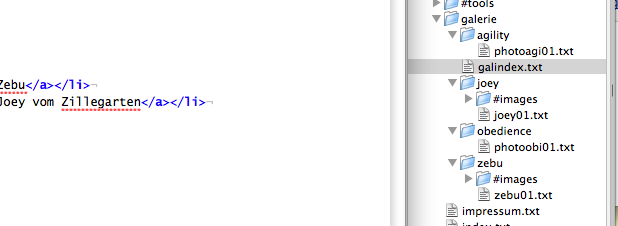
\includegraphics[width=0.7\textwidth]{./images/galerie01.png}
\caption{\label{galerie01}Ordnerstruktur Galerie}
\end{figure}

\begin{itemize}
\item Ordnerstruktur Galerie
\end{itemize}

Also im Klartext und in einer etwas logischeren als der alphabetischen
Reihenfolge, die der Screenshot zeigt, innerhalb des Tutorial-Ordners:


\begin{verbatim}
-- galerie (Ordner)
    -- galindex.txt (Datei)
    -- zebu (Ordner)
        -- #images (Ordner)
        -- zebu01.txt (Datei)
    -- Joey (Ordner)
        -- #images (Ordner)
        -- joey01.txt (Datei)
    -- agility (Ordner)
        -- photoagi01.txt (Datei)
    -- obedience (Ordner)
        -- (photoobi01.txt) (Datei)
\end{verbatim}

In die jeweiligen \#images-Ordner von Zebu und Joey schieben Sie bitte
je die vier zu den Hunden gehörenden Photos hinein.


Und sicher ist Ihnen gleich aufgefallen, daß die Ordner zu Agility und
Obedience keine Bilderordner besitzen. Hier möchte ich Ihnen zeigen,
wie Sie Bilder von externen Webservices einbinden.


Nun nehmen Sie sich die Datei galindex.txt vor und schrieben Folgendes
hinein:


\begin{verbatim}
#title "Galerie"

<h1>Photos aus dem Vereinsleben</h1>

<h2>Unsere Sportarten im Bild</h2>

<ul>
    <li><a href="Photos Agility 1">Agility</a></li>
    <li><a href="Photos Obedience 1">Obedience</a></li>
</ul>

<h2>Unsere Hunde</h2>

<ul>
    <li><a href="Photos Zebu 1">Zebu</a></li>
    <li><a href="Photos Joey 1">Joey vom Zillegarten</a></li>
</ul>
\end{verbatim}

Die einzelnen anderen Datei lassen Sie vorläufig leer. Nur die
Titeldirektive und ein Minimum an Text sollte, um Fehlermeldungen zu
vermeiden, schon einmal hineingeschrieben werden. Die Titel-Direktive
heißt so, wie die jeweiligen Links, die Sie oben in die Listen
eingegeben haben, also schreiben Sie in photoagi01.txt


\begin{verbatim}
#title "Photos Agility 1"

<h1><%= title %></h1>
und in photoobi01.txt

#title "Photos Obedience 1"

<h1><%= title %></h1>
\end{verbatim}

und so weiter …

Bevor Sie sich nun das Ergebnis Ihrer Bemühungen anschauen können,
müssen Sie dafür sorgen, daß es auch in die Navigation eingebunden
ist. Also nehmen Sie sich die Datei \#template.txt vor und ändern die
Navigation, indem Sie einfach den Link zur Galerie noch einfügen:


\begin{verbatim}
<div id="navigation">
    <p><a href="Startseite">Startseite</a> | 
    <a href="Nachrichten">Nachrichten</a> | 
    <a href="Termine">Termine</a> | 
    <a href="Galerie">Galerie</a> | 
    <a href="Impressum">Impressum</a></p>
</div>
\end{verbatim}

Wie immer dient der Umbruch nur der besseren Lesbarkeit und ist nicht
zwingend notwendig.


Wenn Sie jetzt die Seite galindex.txt von RubyFrontier herausschreiben
lassen, sollte Sie so aussehen:

\begin{figure}[h!]
\centering
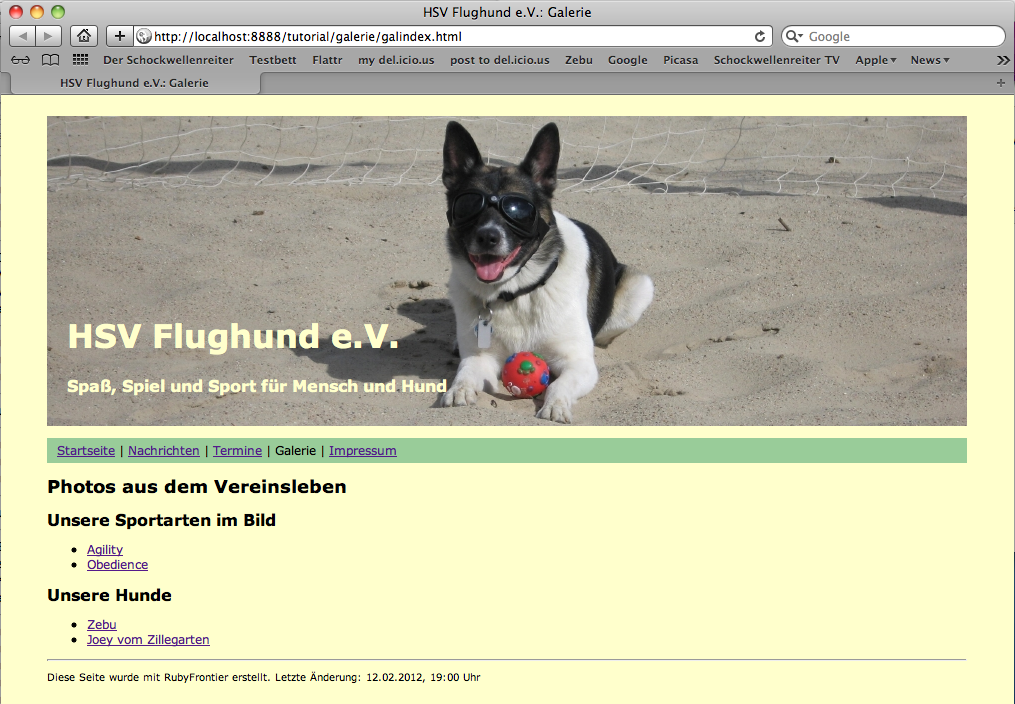
\includegraphics[width=0.7\textwidth]{./images/galerie02.png}
\caption{\label{galerie02}Titelseite Galerie}
\end{figure}

Und wenn Sie nun auch noch alle Seiten herausrendern (was Sie sowieso
müssen, um die Änderungen in der Navigation für alle Seiten wirksam zu
machen), werden Sie feststellen, daß sogar die Links zu den Seiten in
den Unterordnern funktionieren, obwohl wir nirgendwo Unterordner oder
einen Pfad dorthin angegeben haben.


Genau das erledigt RubyFrontier in der Datei autoglossary.yaml
automatisch für uns. Die Software sammelt alle unsere Seiten,
identifiziert sie an den Titeln und speichert die Pfade zu diesen
Seiten ab. Wenn nun ein Link in der Form <a href=''Galerie''>Galerie</a>
auftaucht, identifiziert RubyFrontier dies anhand des fehlenden http
als einen internen Link und schaut in seiner Liste nach dem
Seitentitel, um herauszufinden, wodurch dieser Link zu ersetzen ist,
damit er funktioniert. Eben dies ist der Grund, warum die Seitentitel
eindeutig sein müssen. Die Dateinamen müssen es nicht, theoretisch
kann jeder Unterordner seine eigenen index.txt besitzen. RubyFrontier
findet das jedoch fragwürdig und gibt beim Herausschreiben für jeden
doppelten Dateinamen ein Warnung heraus. Es mag Gründe geben,
Unterordner mit einer eigenen index.html zu versehen und andere
Dateinamen doppelt zu führen, ich versuche dies jedoch durch einen
eindeutigen Prefix (z.B. galindex.txt) zu vermeiden.


Denn RubyFrontier hat einen guten Grund, doppelte Dateinamen
fragwürdig zu finden. Der große Vorteil des Glossary-Mechanismus ist
doch der, daß Sie Unterbäume im Dateibaum ihrer Website beliebig
verschieben, teieln oder auch zusammenfassen können, ohne daß Sie sich
sich um die internen Links kümmern müssen. Einfach einmal alles erneut
herausschreiben und gut ist.


Doch wie Sie vielleicht schon gesehen haben, wenn Sie neugierig die
herausgeschriebene Site inspiziert haben, bewahrt RubyFrontier die
Baumstruktur ihres Projektes: Unterordner im Projekt sind auch
Unterordner (Verzeichnisse) in Ihrer Website. Und wenn Sie jetzt — und
das kommt gar nicht mal so selten vor — Unterordner zusammenfassen
wollen oder müssen und es existieren doppelte Dateinamen, dann geraten
Sie in Teufels Küche.


Daher meine Empfehlung: Beachten Sie die Warnung, die RubyFrontier
herausgibt und vermeiden Sie doppelte Dateinamen. Sie werden mit einer
großen Flexibilität bezüglich der Möglichkeiten, ihre Website
umzuorganisieren, belohnt.


Doch jetzt brennen Sie sicher darauf, Ihre erste Bildergalerie
anzulegen. Nehmen Sie daher die Datei zebu01.txt und schreiben Sie
dieses hinein:


\begin{verbatim}
#title "Photos Zebu 1"

<h1><%= title %></h1>

<%= imageref("zebu01") %>
\end{verbatim}

Wie gewohnt, rendern Sie diese Datei heraus und sie sollte so aussehen:


\begin{figure}[h!]
\centering
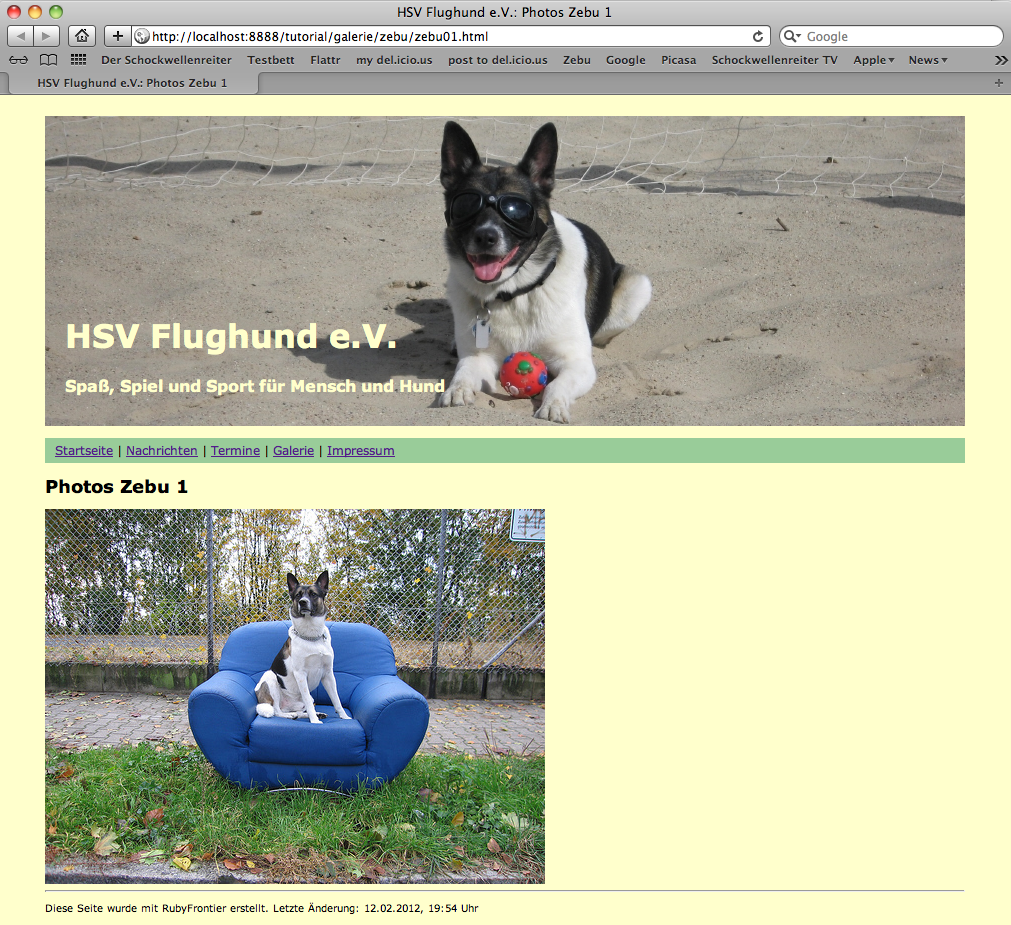
\includegraphics[width=0.7\textwidth]{./images/galerie03.png}
\caption{\label{galerie03}Galerie ohne Stil}
\end{figure}

Okay, seien wir ehrlich. Selbst in den Anfangstagen des Web, als
beinahe jede Scheußlichkeit durchging, wäre diese Seite vom Vorstand
Ihres Sportvereins nicht akzeptiert worden. Zumindest das große Logo
im Kopf der Seite stört und lenkt ganz gewaltig vom Bild ab. Und auch
das Photo sollte mittig erscheinen und etwas mehr Raum gewinnen. Es
ist also an der Zeit für ein alternatives Template!


Also gehen Sie in Ohr Projekt und öffen Sie den
Ordner \#templates. Fall sie darin noch die Dateien secondtemplate.txt
und thirdtemplate.txt finden, können Sie diese löschen. Stattdessen
legen Sie bitte eine Datei namens galerietemplate.txt an. Da ich
schrittweise mit Ihnen das neue Template ausgehend vom
Standard-Template der Website entwickeln möchte, kippen Sie, damit es
einfacher wird, einfach den Inhalt Ihrer \#template.txt-Datei per copy
\& paste dort hinein.


Als erstes löschen Sie dann in dem Galerie-Template das komplette
Header-Div. An diese Stelle kommt nun eine einfache Überschrift mit
dem Titel der Site. Anschließend bauen Sie um den bodytext-Tag
ebenfalls ein div, das Sie mit der id »photogalerie« versehen. Ihr
neues Template sieht dann so aus:


\begin{verbatim}
<%= pageheader() %>
<div class="wrapper">
    <h1><%= sitetitle %></h1>
<div id="navigation">
    <p><a href="Startseite">Startseite</a> |
    <a href="Nachrichten">Nachrichten</a> |
    <a href="Termine">Termine</a> | 
    <a href="Galerie">Galerie</a> | 
    <a href="Impressum">Impressum</a></p>
</div>
<div id="photogalerie">
    <p id="bodytext"></p>
</div>
<hr />
<p class="small">Diese Seite wurde mit RubyFrontier erstellt. 
Letzte Änderung: <%= clocknow() %></p>
</div>
<%= pagefooter() %>
\end{verbatim}

Es ist generell eine gute Idee, den eigentlichen Inhalt der Seite noch
einmal in ein div zu packen, dem man dann noch einmal einen Stil
zuweisen kann.


Jetzt öffnen Sie bitte das Stylesheet und fügen folgende Definition
hinzu:


\begin{verbatim}
#photogalerie {
    margin-top: 30px;
    margin-bottom: 50px;
    margin-left: 100px;
}
\end{verbatim}

Die Werte habe ich experimentell herausgefunden, Sie können also
durchaus damit herumspielen, um ein ästhetisch anspruchsvolleres
Design zu bekommen.


Jetzt fügen Sie noch in die zweite Zeile der Datei zebu01.txt eine
Direktive ein, die RubyFrontier anweist, das alternative Template zu
butzen. (Sie werden später diese Direktive an anderer Stelle
aufschreiben, denn es wäre sicher nicht sinnvoll, diese Zeile in jede
Datei einzufügen, die dieses Template verwenden soll.)


\begin{verbatim}
#template "galerietemplate"
\end{verbatim}

Wenn Sie nun die Seite herausrendern, sollte sie so aussehen:

\begin{figure}[h!]
\centering
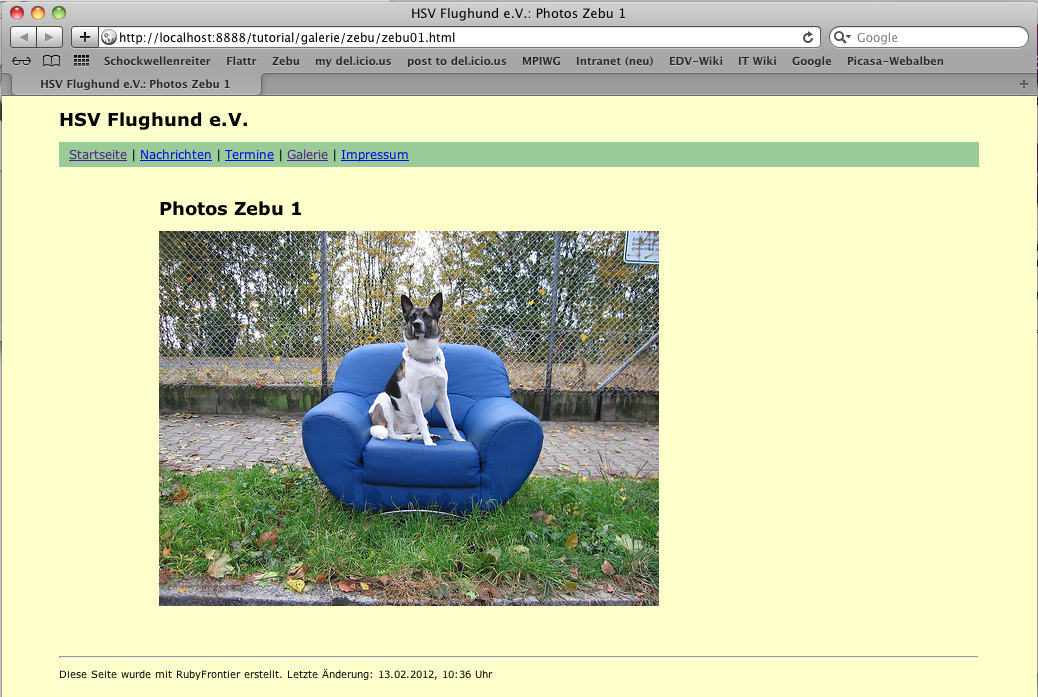
\includegraphics[width=0.7\textwidth]{./images/galerie04.png}
\caption{\label{galerie04}Galerie mit Stil}
\end{figure}

Das kann sich doch schon eher sehen lassen, oder? Jetzt müssen Sie nur
noch die Unschönheit beseitigen, daß die Direktive mit dem
galerietemplate in jeder Datei auftauchen muß. Natürlich können Sie
sich auch hier von RubyFrontier helfen lassen.


In dem Ordner galerie auf gleicher Ebene wie die Datei galindex.txt
legen Sie bitte eine neue, leere Datei mit dem Namen \#prefs.yaml
(inklusive des Doppelkreuzes) an. Und dort schreiben Sie bitte hinein:


\begin{verbatim}
---
:template: galerietemplate
\end{verbatim}

Jetzt können Sie die zuletzt angelegte Direktive in der Datei
zebu01.txt löschen und nach einem erneuten Herausschreiben sollte die
Webseite trotzdem unverändert aussehen.


Was ist passiert? Vor jedem Herausschreiben sammelt RubyFrontier alle
Direktiven, die es findet ein. Einige — aber nicht alle — dieser
Direktiven haben eine kaskadierende Eigenschaft, das heißt, der Wert,
der am nächsten zur gerade herauszuschreibenden Seite steht, wird auf
diese Seite angewendet. Matt Neuburg nennt dies folded (ich habe außer
»kaskadierend« keine wirklich verständliche deutsche Bezeichnung dafür
gefunden). Im Falle des Templates überschreibt der Wert
galerietemplate den globalen Defaultwert template, da die
Datei \#prefs.yaml die Eigenschaft folded besitzt.


Nun legen Sie einfach im Ordner zebu die noch fehldend Dateien
zebu02.txt, zebu03.txt und zebu04.txt an, die genau so aussehen, wie
die erste Datei, nur das die Ziffern in Titel und Bildnamen
entsprechend ausgetauscht werden, also (für die Datei zebu02.txt):


\begin{verbatim}
#title "Photos Zebu 2"

<h1><%= title %></h1>

<%= imageref("zebu02") %>
\end{verbatim}

Bevor Sie nun die Seiten herausrendern, halten Sie einen Moment inne,
da Ihnen sicher aufgefallen ist, daß die einzelnen Seiten der Galerie
ja gar nicht miteinander verlinkt sind. Doch vielleicht erinnern Sie
sich noch an das Makro <\%= nextprevlinks() \%>, welches Sie zu Anfang
aus dem Standard-Template entfernt hatten. Das fügen Sie nun bitte in
das galerietemplate ein, und zwar eine Zeile über dem <hr />:


\begin{verbatim}
</div>
<%= nextprevlinks() %>
<hr />
\end{verbatim}

Rendern Sie nun den Inhalt des Ordners zebu heraus und sie erhalten
vier Seiten mit einer schönen next <-> prev-Navigation unten links:

\begin{figure}[h!]
\centering
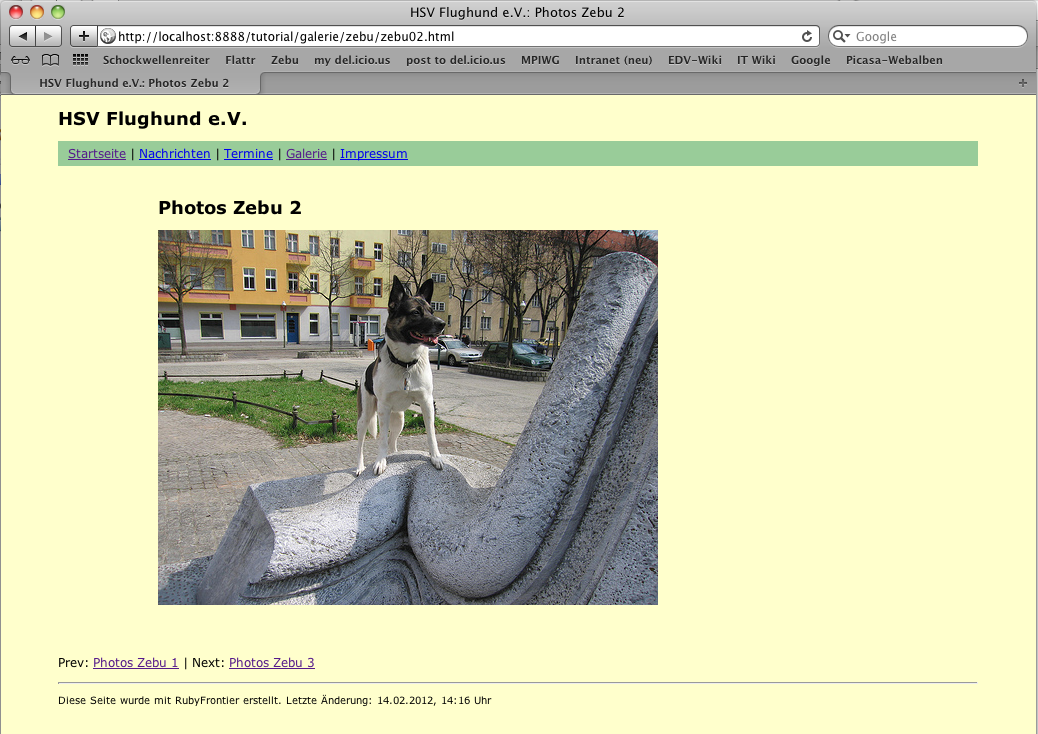
\includegraphics[width=0.7\textwidth]{./images/galerie05.png}
\caption{\label{galerie05}Galerie mit Navigation}
\end{figure}

Sogar die erste und die letzte Seite der Galerie werden erkannt. Es
gibt dort keinen prev- respektive next-Link.


Das die Bezeichnungen englisch sind, nehmen Sie für’s Erste einfach in
Kauf. Ich zeige Ihnen in einem späteren Kapitel, wie Sie diese
Navigation anpassen können. Wichtig zu wissen ist noch, daß
RubyFrontier die Dateien für die Next-Prev-Navigation in
alphabetischer Reihenfolge sortiert — auch dies ist natürlich änderbar
und ich zeige Ihnen später auch noch, wie Sie dies ändern können. Doch
die Galeriebilder liegen ja in der gewünschten Reihenfolge vor, also
können Sie hier einfach das Standard-Marko ohne irgendwelche
Änderungen übernehmen.


Das Anlegen der Galerie »Joey« überlasse ich Ihnen als
Übungsaufgabe. Die erste Datei muß natürlich so aussehen:


\begin{verbatim}
#title "Photos Joey 1"

<h1><%= title %></h1>

<%= imageref("joey01") %>
\end{verbatim}

Beachten Sie bitte, daß Sie auch hier zuerst einmal den ganzen Ordner
(oder alternativ die ganze Site) herausrendern müssen, damit
RubyFrontier die Dateien in seinem Autoglossary aufnehmen und die
Next-Prev-Links herausschreiben kann, andernfalls reagiert die
Software ungehalten mit einer Fehlermeldung. Aber dann sollte Sie auch
eine schöne Sheltie-Galerie besitzen:

\begin{figure}[h!]
\centering
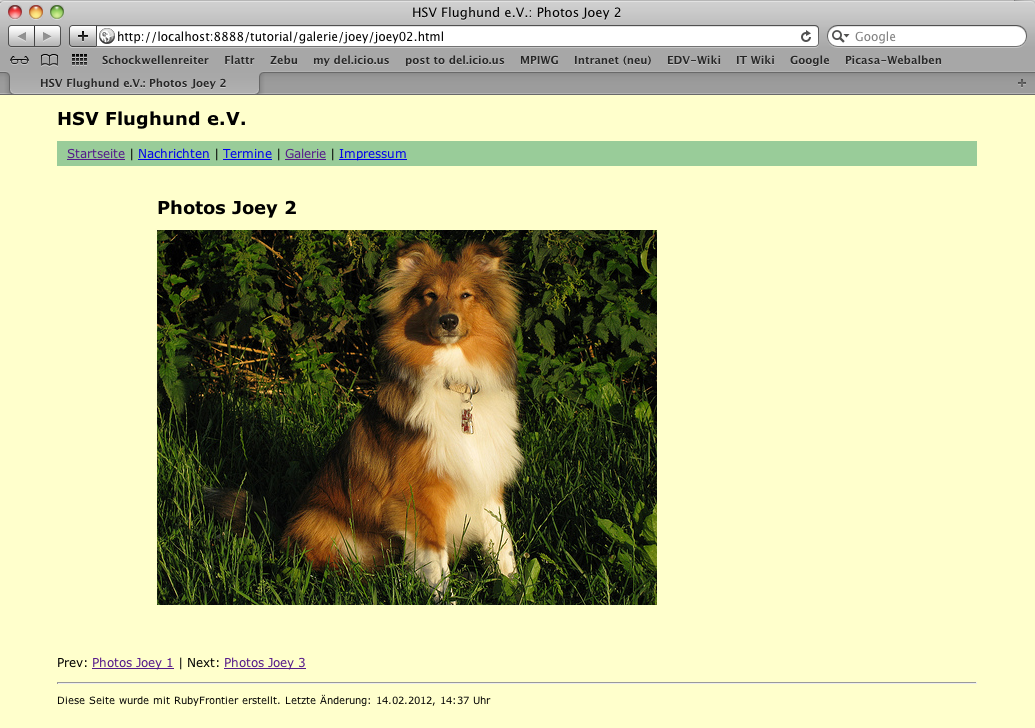
\includegraphics[width=0.7\textwidth]{./images/galerie06.png}
\caption{\label{galerie06}Galerie mit Joey}
\end{figure}

Ein Wort noch zu den Bildern und den \#images-Verzeichnissen. Ob Sie
die Bilder alle in einen großen Bilderordner ablegen oder — wie in
diesem Fall — auf mehrere Ordner verteilen, ist RubyFrontier und dem
imageref-Makro egal. Es Überträgt die Ordnerstruktur so auf den
Server, wie Sie sie angelegt haben. Ich bevorzuge es in diesem Fall,
die Bilder in der Nähe der Seiten zu haben, wo sie eingebunden
werden. Doch das ist sicher auch Geschmackssache. Nur beachten Sie:
Auch das imageref-Makro nimmt bei gleichnamigen Bildern, das was der
gerade herausgeschriebenen Seite am Nächsten liegt, das heißt, auch
der \#images-Ordner ist kaskadierend. Damit lassen sich sogar ganz
nette Tricks realisieren, wie zum Beispiel unterschiedliche
header-Logos je Ordner, wenn jeder Ordner einen \#images-Unterordner
mit zum Beispiel einer eigenen header.jpg-Datei enthält.
\section{Andere Bildquellen}
\label{sec-2-4-1}
\subsection{Photos von Flickr in eine Galerie einbinden}
\label{sec-2-4-1-1}


Der zu Yahoo! gehörende Webservice flickr ist wohl der bekannteste
Service zum Hochladen und und Verteilen von Photographien. Er erlaubt
das komfortable Einbetten von Photos in eigene Webseiten und ist daher
besonders dann eine Alternative, wenn der Speicherplatz bei Ihrem
Provider knapp ist. Ich habe für die Galerie Agility vier Photos von
meinem flickr-Account ausgesucht. (Die Bilder stehen unter einer
Creative-Commons-Lizenz und dürfen daher (bei Namensnennung der
Photographin) für nichtkommerzielle Zwecke eingesetzt werden.)

\begin{figure}[h!]
\centering

\includegraphics[width=0.7\textwidth]{./images/hundebilder03.png}
\caption{\label{hundebilder03}Hundebilder Agility}
\end{figure}

Ein Klick auf die Thumbnails oben öffnet die entsprechende Seite bei
flickr. Dort finden Sie auch den entsprechenden HTML-Code, um das
Photo in Ihre Seite einzubinden:

\begin{figure}[h!]
\centering
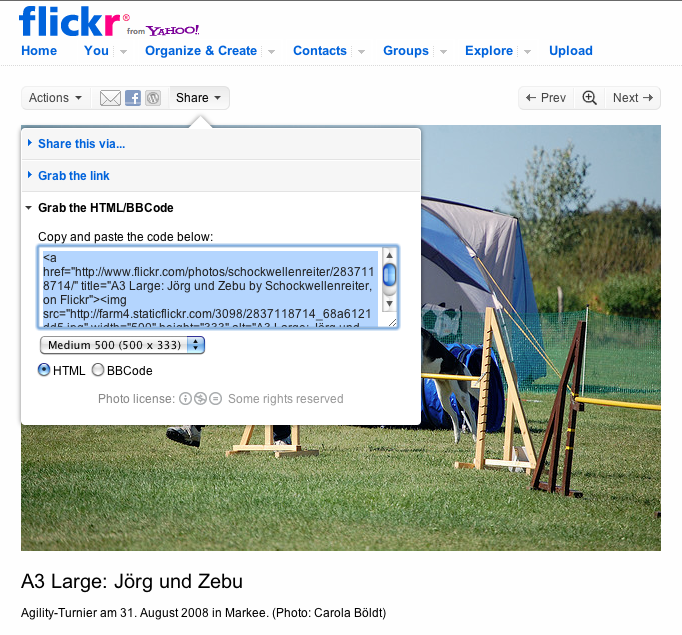
\includegraphics[width=0.7\textwidth]{./images/flickr01.png}
\caption{\label{flickr01}Screenshot Flickr}
\end{figure}


Ich habe die mittlere Größe (500x333 Pixel) ausgewählt. Den Code fügen
Sie bitte ohne Änderungen in die Datei photoagi01.txt im Ordner
agility ein. Mit ein wenig Text drumherum sieht die Seite dann wie
folgt aus:


\begin{verbatim}
#title "Photos Agility 1"

<h1>A3 large: Jörg und Zebu</h1>

<a href="http://www.flickr.com/photos/schockwellenreiter/2837118714/" 
title="A3 Large: Jörg und Zebu by Schockwellenreiter, on Flickr">
<img src="http://farm4.staticflickr.com/3098/2837118714_68a6121dd5.jpg" 
width="500" height="333" alt="A3 Large: Jörg und Zebu"></a>

<p>Agility-Turnier am 31. August 2008 in Markee.
<i>(Photo: Carola Böldt)</i></p>
\end{verbatim}

Wichtig ist, daß der Rücklink auf flickr nicht verändert wird. Die
Geschäftsbedingungen von flickr schreiben dies vor und Yahoo! reagiert
sehr ungehalten mit der Sperrung der Bilder, wenn dies nicht
eingehalten wird.


Mit den übrigen drei Bildern verfahren Sie analog. Überschrift und
Beschreibung können Sie von der flickr-Seite übernehmen. Wenn Sie nun
den gesamten agility-Ordner herausschreiben, erhalten Sie wieder eine
schöne Galerie:

\begin{figure}[h!]
\centering
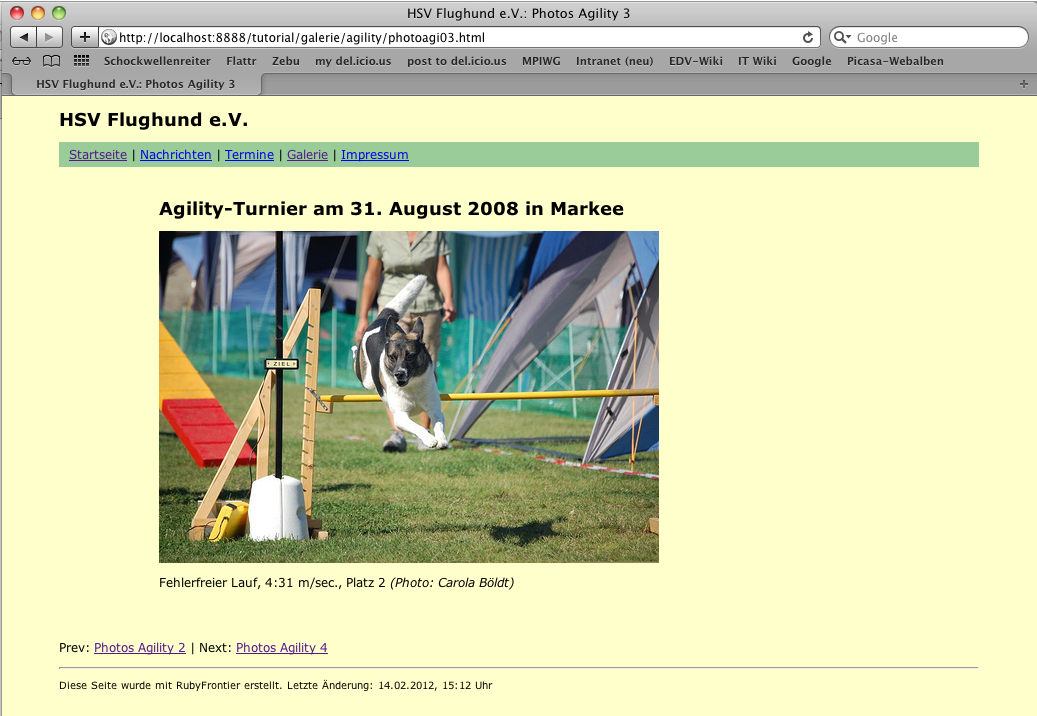
\includegraphics[width=0.7\textwidth]{./images/galerie07.png}
\caption{\label{galerie07}Agility-Galerie}
\end{figure}
\subsection{Picasa Web Albums}
\label{sec-2-4-1-2}


Die Picasa Web Alben sind Googles Antwort auf den Erfolg flickr. Lange
Zeit führten Sie nur ein Schattendasein neben dem Platzhirschen. Aber
seit der Einführung von Google+ hat der Suchmaschinenriese seine
Strategie geändert und Sie können Bilder bis zu einer Größe von 2048 x
2048 Pixeln hochladen, ohne daß dies von dem kostenlosen
Speicherkontingent von 1 Gigabyte abgezogen wird. Bilder, deren
längste Seite 2048 Pixel groß sind, sind für eine Präsentation im Web
allemal ausreichend und so sind die Picasa Web Alben durchaus eine
Alternative zu flickr geworden. Aber beachten Sie bitte: Sie bekommen,
wofür Sie bezahlen, wenn also Google (aber auch Yahoo!) seine
Strategie ändert, kann es durchaus sein, daß die kostenlosen Accounts
auf einmal wieder weg sind.

\begin{figure}[h!]
\centering
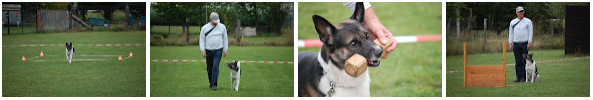
\includegraphics[width=0.7\textwidth]{./images/hundebilder04.png}
\caption{\label{hundebilder04}Hundebilder Obedience}
\end{figure}
                        
Aber egal, ich habe ein paar Obedience-Bilder zu Google hochgeladen
und Sie sollen diese nun in Dateien im Ordner obedience einbinden. Den
Einbettlink finden Sie bei Picasa jeweils rechts unten auf der Seite
des Bildes:

\begin{figure}[h!]
\centering
\includegraphics[width=0.7\textwidth]{./images/picasa01.png}
\caption{\label{picasa01}Screenshot Picasa}
\end{figure}

Den HTML-Code unter »Bild einbinden« kopieren Sie jetzt einfach in die
Seite photoobi01.txt:


\begin{verbatim}
#title "Photos Obedience 1"

<h1><%= title %></h1>

<a href="https://picasaweb.google.com/lh/photo/wdg47Vq08yj_
enKBKxZgxtMTjNZETYmyPJy0liipFm0?feat=embedwebsite">
<img src="https://lh5.googleusercontent.com/-LoOFrVvVcQg/Tzp49KnmOgI/
AAAAAAAACV4/zq3zjHJ8Emw/s800/ob04.jpg" height="297" width="448" /></a>

<p><i>(Photo: Sandra Dittrich)</i></p>
\end{verbatim}

Ich habe auch hier wegen der besseren Lesbarkeit ein paar Umbrüche
vorgenommen, die Sie aber im eigentlichen Code der Seite auf gar
keinen Fall vornehmen dürfen, Sie verändern sonst die URL zu den
Bildern und zum Rücklink.


Google nimmt es übrigens nicht so streng mit dem Rücklink wie
flickr. Wenn nichts Wichtiges dagegenspricht, ist es aber trotzdem ein
Akt der Höflichkeit, den Rücklink zu setzen. Und vergessen Sie bitte
nicht, den Namen der Photographin anzugeben. Es ist bei allen vier
Bildern Sandra Dittrich. Denn auch dies ist ein Akt der Höflichkeit.


Die Seiten photoobi02.txt bis photobi04.txt füllen Sie bitte genau so
aus. Und wenn Sie nun den Ordner herausrendern, haben Sie die letzte
Bildergalerie dieses kleinen Tutorials ebenfalls angelegt.

\begin{figure}[h!]
\centering
\includegraphics[width=0.7\textwidth]{./images/galerie08.png}
\caption{\label{galerie08}Obedience-Galerie}
\end{figure}
\subsection{Selber hosten oder Webservices?}
\label{sec-2-4-1-3}


Das Einbinden von Photos via Webservices wie flickr oder den Picasa
Webalben erscheint auf den ersten Blick äußerst attraktiv,
insbesondere bei quasi kostenlosen Diensten wie Picasa. Es gilt dabei
jedoch zu beachten, daß dies auch mit erheblichen Risiken verbunden
ist: flickr zensiert — speziell in Deutschland. Mein eigener
flickr-Account wurde schon einmal gesperrt, weil dort hochgeladene
Bilder (Abbildungen klassischer Gemälde von Gustave Doré und Georgio
Vasari — das letztere aus dem Jahre 1570 — den Tugendwächtern von
Yahoo! zu nackt waren. Erst nach langwierigem Email-Verkehr und der
(Selbst-) Einstufung dieser Bilder als moderat wurde mein Account
wieder freigeschaltet.

\begin{figure}[h!]
\centering
\includegraphics[width=0.7\textwidth]{./images/zensur.png}
\caption{\label{zensur}Auf Flickr zensierte Bilder}
\end{figure}

Und ich vermute einmal, daß Ihnen dieses auch bei Google passieren
kann. Oder schlimmer noch: Google hat in den letzten Jahren immer
wieder mal Services, die nicht den Erwartungen der Datenkrake
entsprachen, wieder vom Netz genommen. Und wer garantiert Ihnen und
mir, daß dieses nicht auch mit den Picasa Webalben passiert?


Auch wenn in vielen Fällen die Situation nicht so dramatisch ist: Ein
große Vorteil statischer Seiten, wie sie RubyFrontier herausschreibt,
ist der, daß alle Daten in Ihrem Besitz sind und bleiben. Sie sind
weder von Google noch von Yahoo! abhängig. Sicher, flickr wird
vermutlich nie Photos aus dem Leben eines Sportvereins zensieren, aber
schon etwas weniger sicher erscheint mir, ob Google für einen längeren
Zeitraum an den Picasa Webalben festhalten wird. Ohne Zweifel machen
Webservices Spaß und ich nutze Sie auch gerne und viel. Aber überall
dort, wo es Ihnen auf Nachhaltigkeit ankommt, sollten Sie Ihre Daten,
Bilder, Videos (!) — es muß nicht immer YouTube sein — unter Ihrer
Kontrolle behalten.


In dem doch sehr speziellen Fall von Audio- und Video-Dateien werde
ich Ihnen in einem späteren Artikel noch zeigen, wie Sie diese
sinnvoll mit RubyFrontier selber verwalten und in Ihre Seiten
einbinden können.
\section{Der letzter Schliff}
\label{sec-2-4-2}


\begin{figure}[h!]
\centering
\includegraphics[width=0.7\textwidth]{./images/galerie09.png}
\caption{\label{galerie09}Der letzter Schliff}
\end{figure}


Zwei Dinge bleiben meiner Meinung nach noch zu tun, um den Seiten des
fiktiven Hundesportvereins den letztenSchliff zu verpassen. Zum einen
sieht die Startseite der Galerie (galindex) nicht wirklich schön aus,
da auch für Sie nun auch das Template greift, das Sie für die
Photoseiten gescrieben haben. Doch hier ist leicht Abhilfe zu
schaffen. Verschieben Sie einfach die Datei galindex.txt eine Ebene
höher, also auf die gleiche Ebene wie zum Beispiel die index.txt. Und
dann rendern Sie die ganze Site noch einmal neu heraus. Und voila,
alles sieht wieder schick aus. Dank der Hilfe von RubyFroniter müssen
Sie sich keine Gedanken über die internen Pfade etc. machen, das
erledigt die Software für Sie. Und da Sie ja meiner Empfehlung gefolgt
sind und die Seite galindex.txt und nicht index.txt genannt haben, gab
es auch keine Probleme. Verstehen Sie jetzt, warum RubyFrontier eine
Warnung herausgibt, wenn Dateinamen gleich lauten?


Die zweite Änderung ist trivial: In den Galerien wechseln Sie ja die
Navigationsmetapher von einem Linkmenü, wie Sie es in der
Navigationsleiste realisiert hatten, zu den Next-Prevs-Links. Um
klarzustellen, was die nächsthöhere Navigationsebene ist, sollte der
Galerie-Link in der Navigationsleiste hervorgehoben werden. Machen Sie
ihn doch einfach fett, indem Sie den entsprechenden Eintrag im
Galerie-Template wie folgt ändern:


\begin{verbatim}
<b><a href="Galerie">Galerie</a></b>
\end{verbatim}

Das heißt, Sie umgeben den Link einfach noch mit dem entsprechend
HTML-Tag für bold. Das ist generell eine einfache Strategie, um ohne
großen Aufwand eine mehrstufige Navigation zu ermöglichen. Große Sites
können Sie damit so konzipieren, daß Sie bei einer Änderung der
Navigationsstruktur trotzdem nur den entsprechenden (Unter-) Ordner
und nicht die ganze Site neu herausschreiben müssen. Auch darauf werde
ich in einem späteren Kapitel noch einmal zurückkommen.

Nun sind Sie an einem Punkt angelangt, der es Ihnen ermöglicht,
selbstständig mit RubyFrontier zu arbeiten und eigene Sites zu
entwerfen und anzulegen. Auf den nächsten Seiten werde ich auf mehr
fortgeschrittenere Features eingehen, dafür aber die Grundlagen nicht
mehr so ausführlich behandeln. Und dem Hundesportverein Flughund
e.V. sagen Sie hiermit Adieu. Ich hoffe, er ist Ihnen ans Herz
gewachsen. Damit Sie sich ihn noch einmal ansehen können, habe ich die
Seiten hier hochgeladen.
\chapter{Exkurs: RubyFrontier und Amazons S3}
\label{sec-2-5}


Zuerst mußte ich bei meinen Versuchen den Dateinamen index.html noch
explizit anhängen, aber diese Seite hat mir geholfen, Amazon diese
Unart auszutreiben. Der Trick ist folgender:


\begin{enumerate}
\item Das Bucket muß genau so heißen wie die Domain also technisch
   gesprochen, die gleiche CNAME besitzen, in diesem Fall also
   jweb.kantel-chaos-team.de.
\item Dann muß man über die AWS Management Console für dieses Bucket
   festlegen, daß die index.html das Startdokument der Website ist,
   der Welt den Zugriff darauf explizit erlauben und eine Bucket
   Policy erstellen.
\item Die Umleitung der Domain muß auf
   jweb.kantel-chaos-team.de.s3-website-region.amazonaws.com
   erfolgen. Die genaue Region kopiert man sich am einfachsten von der
   Management Console, in meinem Fall war es s3-website-us-east-1.
\end{enumerate}

Und schon hat man eine funktionierende (statische) Website in Amazons
Cloud. Ob und wenn ja, was ich damit anfangen werde, weiß ich noch
nicht. Ich wollte erst einmal nur wissen, ob und wie es geht …
\section{Synchronisieren}
\label{sec-2-5-1}


\begin{figure}[h!]
\centering
\includegraphics[width=0.7\textwidth]{./images/cyberducks3.png}
\caption{\label{cyberducks3}Cyberduck und S3}
\end{figure}
\chapter{RubyFrontier als Autorenwerkzeug}
\label{sec-2-6}


In vielen Projekten, die ich ins Web gestellt hatte, ging es darum,
große Sammlungen historischer Texte, Bilder und anderer Dokumente zu
präsentieren und der (forschenden) Öffentlichkeit zugänglich zu
machen. Prototypisch sei hier auf das Virtual Laboratory (VLP)
hingewiesen, eine Forschungsseite über die Medizingeschichte
des 19. und frühen 20. Jahrhunderts. Diese Site machte auch eine
typische historische Entwicklung durch: Erst wurde sie als statische
Site konzipiert herausgeschrieben mit einer Mixtur aus Frontier und
etlichen handgestrickten Python-Skripten. Nach einiger Zeit wuchs sie
im Umfang und das Herausschreiben dauerte oft eine ganze Nacht oder
länger. So stieg ich auf Zope um, ein damals populäres, in Python
geschriebenes Web Framework, das die einzelnen Seiten dynamisch
herausschrieb und strukturell eine große Ähnlichkeit mit Frontier
aufwies. Mit Zope läuft das VLP heute noch.
\section{The Web is a Writing Environment}
\label{sec-2-6-1}


\begin{figure}[h!]
\centering
\includegraphics[width=0.7\textwidth]{./images/mosaicfrueheversion.jpg}
\caption{\label{mosaicfrueheversion}Erster Mosaic-Browser}
\end{figure}

\begin{itemize}
\item Erster Mosaic-Browser
\end{itemize}

\emph{Das sah übrigens schon Tim Berners-Lee so.}

Doch die Zeit ging weiter und Zope ist schon lange nicht mehr state of
the art. Neben der Tatsache, daß auch einige Zeit die
Weiterentwicklung von Zope auf der Kippe stand, zeigte sich, daß bei
großen Projekten mit vielen Seitenaufrufen sehr schnell
Server-Engpässe auftraten, die es bei statischen Seiten nicht gegeben
hätte. Das größte Problem trat jedoch auf, als mehr und mehr
Wissenschaftler mit dem System arbeiten und in dem System publizieren
wollten. Denn — obwohl das VLP von uns mittlereile zu einem Content
Management System aufgebohrt war, es war nicht wirklich ein writing
environment. Da wurden von einem extra eingerichtetem Redaktionsteam
die (meist als Word-Dokumente) eingesandten Beiträge, mühselig nach
HTML konvertiert, die Links zu den Ressourcen gesetzt und dann in der
Essay-Sektion publiziert.


Und so entstand der Wunsch nach einem Werkzeug, das es den Autoren
leicht macht, für das Web zu publizieren und der Wunsch nach einer
Arbeitsumgebung, die statische Seiten herausschreibt. Ich
experimentierte lange Zeit mit dem Perl Template Toolkit (TT2), das
ein wirklich hervorragendes Werkzeug ist — für Informatiker. Einen
Autoren mit womöglich noch geisteswissenschaftlichem Hintergrund
schreckt es aber eher ab. Wobei ich nicht falsch verstanden werden
möchte: Das Perl Template Toolkit ist ein mächtiges Werkzeug und wer
in die Verlegenheit gerät, Websites mit zehntausenden von Seiten
herausschreiben zu müssen, der sollte sich TT2 durchaus einmal
anschauen.


Ein zweites Beispiel: Als wir am Institut die Edition Open Access
konzipierten (der Prototyp dieser Website wurde von mir übrigens mit
RubyFrontier entwickelt), war uns dieses Problem bewußt. So schufen
wir einen Workflow mit \LaTeX{} als Basis, in die der Autor seine Texte
schreiben sollte. Diese \LaTeX{}-Texte wurden dann mit Hilfe diverser
Werkzeuge und einiger selbstgeschriebener Python-Skripte nach HTML und
EPUB konvertiert. Basis war jedoch das gedruckte Buch.

\begin{figure}[h!]
\centering
\includegraphics[width=0.7\textwidth]{./images/eoa.png}
\caption{\label{eoa}Edition Open Access}
\end{figure}


Das war und ist für die Edition Open Access auch sinnvoll: Die
wissenschaftliche Community hängt am Buch, das ist immer noch der
Nachweis der Arbeit, der auch in Bibliotheken und Bibliographien
verewigt wird. Aber die vielen zusätzlichen Möglichkeiten, die das Web
bietet (Verlinkung, Einbindung multimedialer Inhalte oder Webservices,
die zum Beispiel Übersetzungen der lateinischen Begriffe bieten usw.),
die mußten alle nachträglich und mühsam in die Webseiten eingebaut
werden.


So kam ich auf die Idee, ein Werkzeug für Autoren zu konzipieren, das
es ihnen erlaubt, ihre Texte möglichst einfach selber zu schreiben und
ins Netz zu stellen. Und solch ein Werkzeug möchte ich nun mit Ihnen
gemeinsam entwickeln. Es überrascht Sie sicher nicht, daß die Basis
RubyFrontier ist und daß im Endeffekt so etwas herauskommen wird, wie
diese Website.
\section{Vorüberlegungen}
\label{sec-2-6-2}


RubyFrontier trennt ja, wie viele andere Werkzeuge auch, strikt den
Text, also den eigentlichen Inhalt, von der Präsentation. Alle
Layout-Informationen sind vor dem Autor zu »verstecken«, er soll
komfortabel seinen Text schreiben können, ohne sich um Layout-Dinge
kümmern zu müssen. So kann der Text auch mit diversen anderen Layouts
und auch anderen Werkzeugen bearbeitet werden, um zum Beispiel ein
Ebook oder auch eine gedruckte Version zu erstellen.


Daraus folgt aber auch, daß der Autor nicht mit den Fein- und
Eigenheiten von HTML und seinen diversen Dialekten behelligt werden
sollte. Auch andere XML-basierte Auszeichnungssprachen wie DocBook XML
fallen aus diesen Gründen aus. Doch RubyFrontier bietet mit Markdown
und der Markdown-Erweiterung kramdown eine ernstzunehmende und leicht
zu erlerndene Alternative, die weder am Schreibfluß hindert noch die
Lesbarkeit des Textes erschwert. Daher habe ich sie ausgewählt.


Bei der (Web-) Seitengröße scheiden sich die Geister. Viele Werkzeuge
schreiben jeden kleinsten (Unter-) Abschnitt als eigene HTML-Seite
heraus. Das erhöht zwar die Klickrate, erschwert in meinen Augen aber
die Lesbarkeit, da ich beim Lesen einen größeren Abschnitt auch schon
einmal überfliegen möchte, um dann etwas weiter unten wieder
intensiver nachzulesen. Daher habe ich mich entschieden, jedes Kapitel
auf einer Webseite unterzubringen. Zwar muß man dann beim Lesen der
Seite herunterscrollen, aber ich glaube, daß dies dennoch ein guter
Kompromiß ist, der zudem auch das Ausdrucken der Seiten erleichtert
(nennt mich altmodisch, aber Korrekturlesen mache ich immer noch am
Liebsten auf einem Ausdruck).


Über die Entscheidung ob Markdown oder kramdown nehme ich im nächsten
Abschnitt noch einmal Stellung.


Das Layout der Seite sollte extrem minimalistisch sein und eher an ein
Blatt weißes Papier erinnern, auf das der Autor schreibt. Ich nehme
an, daß während des Schreibvorgangs die Seiten immer wieder einmal
herausgerendert werden, um sie zu lesen oder Links zu testen und
Abbildungen zu überprüfen. Daher sollte nicht allzuviel vom
eigentlichen Text ablenken.


Die meisten Autoren denken, wenn Sie schreiben, seriell das heißt, ihr
Text wird von ersten bis zum letzten Kapitel durchgelesen. Daher soll
eine Navigation eingebaut werden, die ein Vor- oder Zurückblättern
erlaubt. (Das ist aber — besonders für Webpublikationen — nicht
zwingend. Im letzten Beispiel dieses Buches werde ich Ihnen eine
andere, in meinen Augen mehr Web-gerechte Herangehensweise
vorstellen.)


Eine der Forderungen Tim Berners-Lees, des Vaters des World Wide Web,
ist die, daß sich »gute URLs niemals ändern«. Wer schon länger im Web
unterwegs ist, weiß aber auch, daß dies die Forderung ist, gegen die
am häufigsten verstoßen wird. Es gibt einfach viel zu wenig »gute
URLs« im Web. Daher werden Sie lernen, wie Sie mit Hilfe des
Glossary-Mechanismus von RubyFrontier ihre Links so implementieren
können, daß sie wenigstens nur an einer Stelle Änderungen pflegen und
nicht mühselig Seite über Seite überprüfen müssen. Außerdem erfahren
Sie, wie Sie mit Hilfe dieses Mechanismus Querverweise implementieren
können.


Und schließlich soll das Ergebnis dieses Kapitels wiederverwertbar
sein. Denn Sie wollen sicher nicht jedes Mal, wenn Sie ein neues
Projekt beginnen, alles wieder von vorne beginnen. Zum Schluß werden
Sie also ein Template entwickelt haben, eine Blaupause, die Sie immer
wieder neu aufsetzen und für ein Projekt nutzen können.
\section{Ein neues Projekt}
\label{sec-2-6-3}


Legen Sie also los. Bitten Sie RubyFrontier ein neues Projekt
anzulegen. Ich habe es buchprojekt genannt, doch steht es Ihnen
natürlich frei, es so zu benennen, wie Sie wollen. Legen Sie es dort
ab, wo Sie Ihre RubyFrontier-Projekte ablegen möchten und vergessen
Sie nicht, dieses Projekt auch zu sichern.


Dann nehmen Sie sich zuerst die \#ftpSite.yaml vor:


\begin{verbatim}
--- 
:folder: /Applications/MAMP/htdocs/buchprojekt
:method: file
:isLocal: true
:apacheSite: /Applications/MAMP/htdocs/buchprojekt
:apacheURL: http://localhost:8888/buchprojekt/
\end{verbatim}

Mit der ersten Zeile legen Sie wie gewohnt fest, wo RubyFrontier die
herausgeschriebenen Seiten ablegen soll, die beiden letzten Zeilen
brauchen Sie nur, wenn Sie meiner Empfehlung gefolgt sind und mit MAMP
arbeiten. Die zweite und dritte Zeile lassen Sie unverändert, die
benötigt RubyFrontier und Sie sollten sie nie ändern — außer Sie
wissen wirklich genau, was Sie tun.


Jetzt können Sie Ihr Projekt erst einmal komplett herausrendern. Das
empfiehlt sich zu Anfang immer, denn RubyFrontier füllt nun sein
Autoglossary zum ersten Mal.


Im nächsten Schritt passen Sie bitte die Datei \#prefs.yaml an:


\begin{verbatim}
--- 
:bgcolor: ffffff
:sitetitle: 'Mein RubyFrontier-Buchprojekt'
:linkstylesheets: [default]
:markdown: true
\end{verbatim}

Was Sie als sitetitle wählen, bleibt völlig Ihnen überlassen, aber Sie
sehen schon, daß Sie nun ein Stylesheet mit dem Namen default.css
anlegen müssen, um RubyFrontier ohne Fehlermeldung zur Mitarbeit
bewegen zu können.


Und Sie haben mit der letzten Zeile RubyFrontier mitgeteilt, daß Sie
Ihr Buch mit Markdown als Auszeichnungssprache schreiben wollen.
\subsection{Ein komplexeres Stylesheet}
\label{sec-2-6-3-1}


Dazu gehen Sie in den Ordner \#stylesheets ihres Projektes und legen
diese Datei dort an. Und keine Panik: Auch wenn die Überschrift es
ankündigt, sooo komplex ist das Stylesheet dann nun doch nicht:


\begin{verbatim}
body {
    text-align: center; /* IE-Fix */
    font-family: 'Trebuchet MS', Verdana, 'Lucida Grande',
    Arial, Helvetica, sans-serif;
    font-size: 100.01%/1.0;
    color: #111111;
}

pre {
    border: 1px dashed #cccccc;
    padding: 20px 10px;
}

code, pre {
    background-color: #f9f9f9;
    font-family: "Lucida Sans Typewriter", "Monaco",
    "Courier New", Courier, monospace;
    font-size: 90%;
}

.wrapper {
    width: 920px;
    margin: 0 auto;
    text-align: left;
}

.content {
    overflow: hidden;
}

.content .maincontent {
    width: 650px;
    padding-right: 20px;
    float: right;
    display: inline;
}

.content .navbar {
    width: 230px;
    float:left;
    display: inline;
}

.header {
    border-bottom: 1px solid;
}

.header .mylogo {
    float:left;
    margin-right: 10px;
}

.header .mytitle {
    float:left;
}

.footer {
    font-size: 70%;
    border-top: 1px solid;
}
\end{verbatim}

Ich habe wieder wegen der besseren Lesbarkeit ein paar zusätzliche
Zeilenumbrüche bei der Aufzählug der Schriften vorgenommen, im
eigentlichen Stylesheet lassen Sie diese Zeilenumbrüche bitte besser
weg.

Es ist eigentlich immer noch ein ziemlich minimalistisches
Stylesheet. Sie erkennen sicher, daß es ein Zweispaltenlayout anlegt,
mit einer 230 Pixel breiten, linken Navigationsspalte und einer 650
Pixel breiten Hauptspalte für den eigentlichen Inhalt. Spielen Sie
ruhig damit, es ist sicher noch verbesserungsfähig. Denn ich bin nicht
wirklich ein CSS-Guru.
\subsection{Das Template}
\label{sec-2-6-3-2}


Bevor Sie nun mit dem Template beginnen, kopieren Sie sich bitte diese
beiden Bilder in den \#images-Ordner Ihres Projektes,

\begin{figure}[h!]
\centering
\includegraphics[width 5cm]{./images/widgets.png}
\caption{\label{widgets}Widgets}
\end{figure}

damit RubyFrontier Sie auch finden kann. Sie können Sie auch
umbenennen (dann müssen Sie es aber auch im Template ändern), aber per
Default heißen Sie cc80x15.png und rubyfrontierbadge.png.


Als nächstes können Sie die Datei \#pageheader.txt anlegen. Sie ist
nicht unbedingt notwendig, außer dem Zusatz, daß die Sprache deutsch
ist, ist es der Standard-Pageheader, der in RubyFrontier als Default
fest verdrahtet ist. Aber ich habe lieber einen eigenen Pageheader,
über den ich die Kontrolle habe und den ich gegebenenfalls auch
erweitern kann. Im Falle dieser Seite habe ich hier zum Beispiel auch
noch das JavaScript für den Flattr-Button eingebaut. Und natürlich
besteht der Titel aus dem Titel der Seite und dem Site-Titel:


\begin{verbatim}
<!DOCTYPE html PUBLIC "-//W3C//DTD XHTML 1.0 Transitional//EN"
    "http://www.w3.org/TR/xhtml1/DTD/xhtml1-transitional.dtd">
<html xmlns="http://www.w3.org/1999/xhtml" xml:lang="de" lang="de">
<head>
    <%= metatags() %>
    <%= linkstylesheets() %>
    <%= linkjavascripts() %>
    <title><%= sitetitle %>: <%= title %></title>
</head>
<%= bodytag() %>
\end{verbatim}

So, und nun endlich das Template. Es ist schon etwas komplexer, aber
ich werde die einzelnen Stellen mit Ihnen Schritt für Schritt
durchgehen:


\begin{verbatim}
<%= pageheader() %>
<div class="wrapper">
    <div class="header">
        <div class="mylogo">
            <a href="index.html">
                <%= imageref("rubyFrontierLogo", {:border => "0", 
                :alt => "RubyFrontier Logo", :width => "59", :height => "64"}) %>
            </a>
        </div>
        <div class="mytitle">
            <h1><%= sitetitle %></h1>
        </div>
        <br clear="all" />
    </div>
    <div class="content">
        <div class="maincontent">
            <!-- begin content -->
            <p id="bodytext"></p>
            <!-- end content -->
        </div>
        <div class="navbar">
            <h4>Navigation</h4>
            <!-- hier kommt die Navigation hin -->
        </div>
    </div>
    <%= nextprevlinks() %>
    <div class="footer">
        <p>(<a href="http://creativecommons.org/licenses/by-nc-sa/3.0/de/">cc</a>)
         2011-<%= yearnow() %> -- Some Rights Reserverd -- Letze Änderung: 
        <%= clocknow() %></p>
        <p>
            <!-- RubyFrontier -->
            <a href="http://www.apeth.com/RubyFrontierDocs/default.html">
            <%= imageref("rubyfrontierbadge", {:width => "80", :height => "15", 
            :alt => "RubyFrontier Badge", :title => "Made with RubyFrontier", 
            :border => "0"}) %></a>
            <!-- Ende RubyFrontier -->
            &nbsp;
            <!-- CC-Button -->
            <a href="http://creativecommons.org/licenses/by-nc-sa/3.0/de/">
            <%= imageref("cc80x15", {:width => "80", :height => "15", 
            :alt => "CC Logo", :title => "CC BY NC SA", :border => "0"}) %></a>
            <!-- Ende CC-Button -->
        </p>
    </div>
</div>
<%= pagefooter() %>
\end{verbatim}

Auch hier habe ich wieder aus Gründen der Lesbarkeit ein paar
zusätzliche Zeilenumbrüche vorgenommen.


Mit diesen Änderungen können Sie die Seite firstpage.txt probeweise
einmal von RubyFrontier herausschreiben lassen. Sie sollte dann so
aussehen:

\begin{figure}[h!]
\centering
\includegraphics[width=0.7\textwidth]{./images/buchprojekt01.png}
\caption{\label{buchprojekt01}Screenshot 1}
\end{figure}

Daß die Seite korrekt herausgeschrieben wird, obwohl sie keine einzige
Markdown-Auszeichnung erhält, liegt daran, daß Markdown beliebigen
HTML-Code enthalten darf, der ohne Änderung vom Markdown-Interpreter
durchgereicht wird.


Doch jetzt zum Template: Die ganze sichtbare Seite ist in einem
Wrapper geklammert, der via Stylesheet dazu gebracht wurde, die Breite
auf 920 PIxel festzulegen und zu zentrieren. Dann kommt der Header,
der links das Logo einbindet und rechts daneben den Sitetitle
anzeigt. Sie können natürlich ein Logo Ihrer Wahl nehmen, müssen
natürlich dann den Namen der Datei anpassen oder im Template
ändern. Im Prinzip geht jedes Bild, das etwa 60 bis 65 Pixel hoch
ist. (Die Breite ist relativ egal und höchstens ein ästhetisches
Problem.)


Dann kommt der eigentliche Inhalt und die Navigation (wie Sie diese
realisieren erfahren Sie weiter unten).


Und schließlich noch der Footer, dem Sie stolz ein RubyFrontier-Badget
verpaßt haben und dort ist auch die Stelle, an der Sie dem geneigten
Leser mitteilen, daß Ihre Seiten unter einer Creative Commons Lizenz
zur Verfügung stehen. Es bleibt natürlich Ihnen überlassen, weitere
Buttons hinzuzufügen oder wegzulassen. Ich habe auf meinen Seiten —
also auch hier — zusätzlich noch ein Statistik Tool und den
Flattr-Button (eine Micro-Payment-Dienst) eingebaut. Auf Letzeren
können Sie klicken, wenn Sie mir etwas Gutes tun wollen.
\subsection{Navigation}
\label{sec-2-6-3-3}


Doch nun zur Navigation. Damit Sie überhaupt navigieren können, müssen
Sie natürlich erst einmal ein paar Seiten anlegen, zwischen denen Sie
hin- und herspringen wollen. Löschen Sie daher erst einmal alle
Seiten, die Matt Neuburg angelegt hat, also firstpage, secondpage und
thirdpage. Sie benötigen Sie nicht mehr. Stattdessen legen Sie eine
Seite index.txt, kapitel01.txt und kapitel02.txt an, die Sie mit ein
wenig Blindtext füllen (ich benutze dafür der Einfachheit halber immer
diesen Blindtext-Generator).


Sie werden dabei feststellen, daß die Seiten ohne Überschrift
dargestellt werden — falls Sie nicht so klug waren, und Ihr schon
welche verpaßt hatten. Denn sicher haben Sie gemerkt, daß im Template
vor dem bodytext kein Titel-Makro der Form <\%= title \%> steht. Der
Grund ist, daß ich die Erfahrung gemacht habe, daß die
Kapitelüberschriften — speziell in wissenschaftlichen Werken — doch
oft eine erhebliche Länge aufweisen, der Titel aber, da er in der
Kopfleiste des Browser erscheint und auch in der noch zu erstellenden
Navigation, meist kürzer gewünscht wird.


Ich habe in meinem Beispiel die Titel Startseite, Kapitel 1 (mit einer
langen Kapitel-Überschrift) und Kapitel 2 (mit einer kürzeren
Kapitelüberschrift) gewählt.


Wenn Sie nun einfach alle drei Seiten herausschreiben, werden Sie
feststellen, daß — wie durch ein Wunder — die Navigation auf die
vorherige und nächste Seite funktioniert.

\begin{figure}[h!]
\centering
\includegraphics[width=0.7\textwidth]{./images/buchprojekt02.png}
\caption{\label{buchprojekt02}Screenshot 2}
\end{figure}


Natürlich ist es kein Wunder, sondern es liegt daran, daß
RubyFrontier, solange Sie der Software nichts anderes sagen, die
alphabetische Reihenfolge der Dateinamen für die Navigation
annimmt. Hätten Sie die Kapitel-Seiten statt kapitel01 etc. chapter01
genannt, dann wäre Ihnen die schöne Reihenfolge völlig durcheinander
geraten.


Um RubyFrontier also die Reihenfolge mitzuteilen, benötigen Sie eine
Direktive namens \#nextprevs, für die Sie am Besten die
Datei \#nextprevs.txt anlegen. Und dort schreiben Sie einfach die
Kapitel in der korrekten Reihenfolge untereinander hinein, also in
diesem Fall


\begin{verbatim}
Startseite
Kapitel 1
Kapitel 2
\end{verbatim}

oder wie immer Sie die Titel der einzelnen Seiten gewählt haben. Sie
können übrigens statt der Titel auch die Dateinamen (ohne die Endung
.txt) dort hineinschreiben, RubyFrontier sucht sich das Richtige schon
heraus. In diesem Fall sähe es dann so aus:


\begin{verbatim}
index
kapitel01
kapitel02
\end{verbatim}

Welche der beiden Versionen Sie nehmen, ist Geschmacksache. Ich
persönlich bevorzuge die zweite Fassung, da ich während des
Entstehungsprozesses eines Buches schon häufiger mal die Titel
wechsle, aber eigentlich nur noch sehr selten die Dateinamen.


So, und nun wollen Sie sicher die leere Navigationsspalte
auffüllen. Dazu habe ich ein Ruby-Makro, das Matt Neuburg im Quelltext
zur RubyFrontier-Dokumentation mitliefert, gnadenlos
vereinfacht. Legen Sie also im Ordner \#tools eine Datei navbar.rb an
und schreiben Sie dort folgendes hinein:


\begin{verbatim}
def navbar()
  dirname = adrSiteRootTable
  embed_in_template(process(dirname))
end

def process(dir)
  arr = Array.new
  html.pagesInFolder(dir).each do |what|
    title, path = html.getTitleAndPaths(what)
    s = html.getLink(title, what)
    arr << "<li>" + s + "</li>\n"
  end
  arr
end

def embed_in_template(arr)
  return "" unless arr
  ss = <<END
  <ul class="nav">
  #{arr}
  </ul>
END
  ss
end
\end{verbatim}

Was macht nun dieses Makro? Es liest alle Seiten in einem Ordner
heraus — das Buchprojekt geht davon aus, daß Sie keine Unterordner
benutzen — und bastelt daraus eine Liste mit Links. Und jetzt kommt
der Trick: Wenn eine \#nextprevs-Direktive existiert, lädt das Makro
diese und behält auch die Reihenfolge.


Übrigens lohnt es sich durchaus, den Quelltext der Dokumentation
ausführlich zu studieren (sie können ihn sich im Bundle-Menü unter
Show RubyFrontier Docs Source in TextMate anzeigen lassen). Dort sind
schon viele Lösungen vorhanden, von denen Sie sich inspirieren lassen
können.


Nun müssen Sie nur noch das Template öffnen und unter das Makro an der
korrekten Stelle einfügen:


\begin{verbatim}
<div class="navbar">
    <h4>Navigation</h4>
    <%= navbar() %>
</div>
\end{verbatim}

Wenn Sie nun wieder alle Seiten herausschreiben lassen, sehen Sie
links die gewünschte Navigationsleiste. Wenn Sie wollen, können Sie
diese natürlich mit ein paar CSS-Spielereien noch ein wenig
aufhübschen, mir reicht sie so jedoch aus.


Was mich aber noch störte, waren die englischen Wörter Next und Prev
in der Vorwärts-/Rückwärts-Navigation links unten. Für die ist das
(mitgelieferte) Makro nextprevlinks() verantwortlich, das im Original
so aussieht:


\begin{verbatim}
def nextprevlinks()
  p, n = html.getNextPrev(adrObject)
  ntitle, npath = html.getTitleAndPaths(n) if n
  ptitle, ppath = html.getTitleAndPaths(p) if p
  rel_to_top = adrsiteroottable.relative_uri_from(adrobject)
  s = ""
  s << "Prev: " + html.getLink(ptitle, rel_to_top + ppath) if p
  s << " | " if p and n
  s << "Next: " + html.getLink(ntitle, rel_to_top + npath) if n
  "<p>#{s}</p>\n"
end
\end{verbatim}

Selbst Menschen, die in Ruby nicht so bewandert sind, erkennen sofort
die Stellen, an denen Änderungen vorgenommen werden müssen, um die
Navigation zu internationalisieren. Ich hatte beschlossen, statt der
englischen Begriffe einfach je zwei Doppelpfeile zu setzen (<<
>>). Dies ist — glaube ich — international verständlich. Mit meinen
Änderungen sieht das Makro dann so aus:


\begin{verbatim}
def nextprevlinks()
  p, n = html.getNextPrev(adrObject)
  ntitle, npath = html.getTitleAndPaths(n) if n
  ptitle, ppath = html.getTitleAndPaths(p) if p
  rel_to_top = adrsiteroottable.relative_uri_from(adrobject)
  s = ""
  s << "<< " + html.getLink(ptitle, rel_to_top + ppath) if p
  s << " | " if p and n
  s << html.getLink(ntitle, rel_to_top + npath) + " >>" if n
  "<p>#{s}</p>\n"
end
\end{verbatim}

Jetzt rendern Sie noch einmal alle Seiten heraus. Sie sollten von der
Struktur her nun nahezu identisch mit diesen Seiten sein:

\begin{figure}[h!]
\centering
\includegraphics[width=0.7\textwidth]{./images/buchprojekt03.png}
\caption{\label{buchprojekt03}Screenshot 3}
\end{figure}

Im Prinzip könnten Sie nun loslegen und Ihr Meisterwerk schreiben. Es
ist nun alles dafür vorhanden. Daher werde ich Ihnen als Nächstes
zeigen, wie Sie Ihre Seiten mit Markdown als Auszeichnungssprache
füllen oder ob Sie besser kramdown dafür nutzen.
\chapter{Markdown und kramdown}
\label{sec-2-7}


Markdown ist eine von John Gruber und Aaron Swartz entwickelte,
einfache Auszeichnungssprache mit dem Ziel, schnell und komfortabel
Webseiten zu erstellen, ohne sich mit den Tücken von HTML
herumschlagen zu müssen. Dabei sollte der Text für Menschen leicht
lesbar bleiben. Die Referenzimplementierung ist in der Skriptpsrache
Perl geschrieben und RubyFrontier ruft dieses Perl-Skript auf.


Markdown hatte nie das Ziel, HTML zu ersetzen, an allen Stellen, an
denen Markdown nicht ausreicht, kann man HTML einsetzen, das der
Markdown-Interpreter einfach unangetastet durchreicht. Markdown ist
mittlerweile so etwas wie ein (Quasi-) Standard, es existieren
Implementierungen in vielen anderen Skript- und Programmiersprachen
und es gibt etliche Erweiterungen, von denen eine — nämlich kramdown
durch RubyFrontier von Hause aus unterstützt wird.


Es ist nicht Ziel des Kapitels, die komplette Syntax von Markdown
vorzustellen, dazu gibt es eine hervorragende deutschsprachige
Webseite, ich möchte nur die wichtigsten Elemente vorstellen, die ich
tagtäglich nutze:




\begin{verbatim}
# Das ist eine H1-Überschrift und
## Das eine H2-Überschrift
\end{verbatim}

das geht natürlich weiter bis H5. Textauszeichnungen sind auch möglich:


\begin{verbatim}
**dieser Text wird fett dargestellt** und *dieser Text kursiv*
und so sieht ein [Link zur
RubyFrontier-Dokumentation](http://www.apeth.com/RubyFrontierDocs/default.html)
aus.
\end{verbatim}

In RubyFrontier kann man interne Links natürlich auch abkürzen:


\begin{verbatim}
Hier geht es zur [Startseite](Startseite)
\end{verbatim}

Text, der mit einem Tabulatorschritt eingerückt ist, wird als
Quelltext behandelt, also in einem <code><pre>-Block
eingeschlossen. Um das eventuelle Maskieren von reservierten Zeichen
kümmert sich Markdown selber. Das gilt auch für Inline-Code-Elemente,
die zwischen zwei Backticks (`) eingeschlossen werden.


Listen gehen auch. Zunächst eine ungeordnete Liste:


\begin{verbatim}
* Listenpunkt 1
* Listenpunkt 2
\end{verbatim}

wird zu

\begin{itemize}
\item Listenpunkt 1
\item Listenpunkt 2
\end{itemize}

Dabei ist zu beachten, daß zwei Leerzeichen vor dem Stern stehen müssen.

Geordnete (durchnumerierte) Listen sehen ähnlich aus. Auch zwei
Leerzeichen einrücken und dann


\begin{enumerate}
\item Listenpunkt 1
\item Listenpunkt 2
\end{enumerate}

schreiben. Das ergibt das gewünschte Ergebnis:


Listenpunkt 1
Listenpunkt 2

Die Reihenfolge der Ziffern und welche gewählt wird, ist dabei völlig
unerheblich. Auch


\begin{enumerate}
\item Listenpunkt 1
\item Listenpunkt 2
\end{enumerate}

wird zu

Listenpunkt 1
Listenpunkt 2

Die korrekte Numerierung übernimmt Markdown für uns. Das ist manchmal
recht nützlich, wenn man nachträglich in einer großen Liste noch
einige Punkte einfügen muß.


Das ist eigentlich alles, was ich benötige und was ich mir gemerkt
habe, denn für Bilder nutze ich RubyFrontiers <\%= imageref()
\%>-Makro. Brauche ich doch einmal mehr, schreibe ich dies entweder
direkt in HTML (z.B. Tabellen) oder ich schaue doch einmal im
Syntax-Manual nach.


Es gibt (mindestens) zwei Probleme, die bei der Nutzung des
Markdown-Interpreters auftreten. Links mit Klammern, wie sie zum
Beispiel in der Wikipedia häufig vorkommen
(\href{http://de.wikipedia.org/wiki/Pascal_(Programmiersprache)}{http://de.wikipedia.org/wiki/Pascal\_(Programmiersprache)}) werden in
Markdown nicht korrekt interpretiert, die schließende Klammer ist
nicht mehr Teil des Links, der daher dann in die Leere geht. Als
Workaround kann man an dieser Stelle direkt mit HTML arbeiten, also
zum Beispiel


<a href=''\href{http://de.wikipedia.org/wiki/Pascal_(Programmiersprache)}{http://de.wikipedia.org/wiki/Pascal\_(Programmiersprache)}''>Pascal</a>
schreiben, schön ist dies natürlich nicht. Andere
Markdown-Implementierungen und/oder -Erweiterungen wie kramdown haben
diesen Fehler nicht. Das gilt auch für das zweite Problem:


Da nicht nur das Sternchen (*), sondern auch der Unterstrich ($_)$
genutzt werden kann, um Text kursiv zu setzen, sind Unterstriche in
Links und Dateinamen problematisch (auch im <\%= imageref()
\%>-Makro). Das ist ärgerlich, da Unterstriche speziell in Dateinamen
für Bilder häufig vorkommen. Aber es gibt nur einen Lösung (wenn man
mit Markdown arbeiten will): Alle Unterstriche in Dateinamen zum
Beispiel durch Bindestriche ersetzen. Die sind unproblematisch. Auch
dieser Fehler tritt in kramdown nicht auf.
\section{Doch was ist mit Fußnoten?}
\label{sec-2-7-1}


Jetzt haben Sie mich erwischt! Fußnoten kann Markdown nicht! Vermutlich haben die Schöpfer von Markdown Fußnoten als etwas dem Web völlig Fremdes angesehen und deshalb darauf verzichtet. Eine Aussage, die ich durchaus unterstreichen kann. In der Besten aller Welten kommen Fußnoten auf Webseiten nicht vor. Nur leider leben wir nicht in der Besten aller Welten und auch ich habe einige Projekte, die ohne Fußnoten nicht auskommen. Und so habe ich es mit kramdwon versucht. In der Theorie war dies auch recht einfach: Sie müssen bloß in der \#prefs.yaml


\begin{verbatim}
:markdown: true
\end{verbatim}

durch


\begin{verbatim}
:kramdown: true
\end{verbatim}


ersetzen und schon flutscht alles. Denn RubyFrontier kümmert sich um
alles andere und nimmt in diesem Fall den kramdown-Interpreter. Doch
leider erlebte ich einige unschöne Überraschungen: RubyFrontier ruft
in der Default-Implementierung den Markdown-Interpreter im pageFilter
auf und der arbeitet auf dem :bodytext, also ohne das ganze HTML des
Templates drumherum. kramdown dagegen wird im postMacroFilter
aufgerufen, da das mächtigere kramdown einige unschöne Sachen mit den
Makros anstellt (genauer: Es setzt »intelligente« Anführungszeichen
statt der doppelten Hochkommata). Abgesehen davon, daß »intelligente«
Anführungszeichen außerhalb der anglo-amerikanischen Welt nie eine
gute Idee sind, da fast jede Sprache eigene Anführungszeichen besitzt
(zum Beispiel in Deutschland „“, in Frankreich »« und in der Schweiz
«» — oder umgekehrt), ist das natürlich katastrophal für Makro-Aufrufe
etc. Deshalb der Aufruf nach der Makro-Ersetzung. Doch damit rennt man
natürlich in folgende zwei Probleme:


Der postMacroFilter arbeitet mit dem :postMacroText, und das ist der
Text inklusive des vollständigen Templates, da in den Templates ja
ebenfalls Makros vorkommen dürfen. Und was passiert, wenn man
ordentlich eingerückte Templates geschrieben hat und man kramdown, das
ja im Prinzip eine Erweiterung von Markdown ist, mit Tabstops
eingerückten HTML-Quelltext vorsetzt? Richtig! kramdown behandelt dies
als Code und legt einen <code><pre>-Block drumherum. (Es gibt Tricks,
der Software dieses Verhalten abzugewöhnen — zum Beispiel auf
Einrückungen verzichten —, aber schön ist es trotzdem nicht).

Schlimmer aber ist: kramdown schreibt den Text der Fußnoten ganz unten
an den Fuß der Seite, also noch unterhalb des Footers mit den
Copyright-Vermerk und den schönen Buttons, statt sie an das Ende des
Content-Blocks zu schreiben. Dieses Verhalten ist nicht wirklich der
Software anzulasten, denn woher soll sie wissen, wo der Content endet
und das Template anfängt?
\section{RubyFrontier und kramdown}
\label{sec-2-7-2}


Nach langen Überlegungen habe ich mich dennoch entschieden, das
Markdown-Superset kramdown, in den meisten meiner
RubyFrontier-Projekte einzusewtzten. Und das aus zwei Gründen:

\begin{itemize}
\item (John Grubers Original-) Markdown hat zwei kleinere Bugs: So kann
  die Software nicht vernünftig mit Links umgehen, die Klammern
  enthalten, wie sie zum Beispiel in der Wikipedia häufiger vorkommen
  (\href{http://de.wikipedia.org/wiki/Java_(Programmiersprache)}{http://de.wikipedia.org/wiki/Java\_(Programmiersprache)}). Hier
  glaubt Markdown einfach, die Klammer hinter Programmiersprache wäre
  das Ende der Linkauszeichnung und liefert daher den Link in der Form
  \href{http://de.wikipedia.org/wiki/Java}{http://de.wikipedia.org/wiki/Java}_(Programmiersprache, also ohne die
  letzte Klammer. Außeredem kann man in Markdown ja kursiven Text auch
  darstellen, indem man nicht nur Sternchen, sondern auch je einen
  Unterstrich vor und nach dem Text setzt, also \underline{dieser Test ist   kursiv} wird zu »dieser Text ist kursiv«. Markdown interpretiert
  aber auch Unterstriche in Links, wenn sie mindestens zwei mal
  vorkommen, als Anweisung, dieses als kursiven Text zu behandeln und
  verhaut so die Links: Aus www.meine$_{\mathrm{tolle}}$$_{\mathrm{webseite}}$ wird
  www.meine<em>tolle</em>webseite. Für beides gibt es Workarounds,
  aber schön ist es nicht.
\item Markdown hat keine Befehle für Fußnoten, kramdown schon. Und auch
  wenn ich Fußnoten als etwas betrachte, das dem Web ferne steht1, im
  wissenschaftlichen Bereich kommt man bis heute einfach nicht darum
  herum.
\end{itemize}

Daher hatte ich mich entschieden, kramdown zu nutzen, das von Matt
Neuburg ja auch wärmstens empfohlen wird2.

Doch zuerst rannte ich dabei nur in Probleme. Das kleinste dabei war,
daß kramdown weder zur Standard-Ruby-Installation auf dem Mac gehört,
noch daß es mit RubyFrontier mitgeliefert wird.

\begin{figure}[h!]
\centering
\includegraphics[width=0.7\textwidth]{./images/installingkramdown.png}
\caption{\label{installingkramdown}kramdown installieren}
\end{figure}


Doch


\begin{verbatim}
sudo gem install kramdown
\end{verbatim}

erledigt dies zuverlässig auf jedem Mac.

Schwieriger war das nächste Problem. Da kramdown Seltsames mit den
Makro-Aufrufen anstellt, hatte sich Matt entschieden, im Gegensatz zu
Markdown, das im pageFilter aufgerufen wird, kramdown erst im
postMacroFilter aufzurufen. Das führte bei mir jedoch zu zwei
ärgerlichen Nebeneffekten:


\begin{enumerate}
\item Der postMacroFilter arbeitet auf der gesamten Webseite, also auf
   dem bodytext wie auf dem umgebenden Template. Das ist natürlich
   logisch, da ja auch das Template Makros enthalten kann. Nun erkennt
   aber dummerweise kramdown (wie auch Markdown) eingerückten Text als
   Quelltext und behandelt ihn auch als solchen, das heißt also, statt
   den Footer dieser Seite als HTML zu behandeln, schrieb kramdown
\end{enumerate}


\begin{verbatim}
<br />
<div class="footer">
<p>(<a href="http://creativecommons.org/licenses/by-nc-sa/3.0/de/">cc</a>) 2012-<%= yearnow() %> -- Some Rights Reserverd -- Letze Änderung: 07.11.2013, 11:48 Uhr -- <a href="Impressum">Impressum</a> -- <a href="RSS-Feed">RSS-Feed</a></p>
<p> …
\end{verbatim}

heraus. Die Alternative wäre natürlich, im Template auf Einrückungen
zu verzichten, aber ich liebe nun einmal sauber eingerückten
Quellcode, daher war diese Alternative für mich keine.


\begin{enumerate}
\item kramdown schreibt die Fußnoten an das Ende des Textes, den der
   Interpreter abarbeitet. Das heißt also, wenn man dann auf
   Einrückungen verzichtet, erschienen die Fußnoten nach dem Footer,
   also im Falle dieses Notizheftes unterhalb des Flattr-Buttons. Das
   ist natürlich ebenfalls hoch unerwünscht, Fußnoten sollten da
   erscheinen, wo Ihr sie in dieser Worknote unten auch seht.
\end{enumerate}


Daher erschien mir die einzig vernünftige Alternative, kramdown
ebenfalls im pageFilter aufzurufen3. Dann funktionierten aber die
Makros nicht mehr, da kramdown einige Substitionen vornimmt. Nun kann
man kramdown aber auch von der Kommandozeile aus aufrufen, und daher
habe ich mir dort angeschaut, was die Software eigentlich mit den
Makro-Aufrufen anstellt. Und das war eigentlich ziemlich eindeutig,
aus


\begin{verbatim}
<%= imageref("pussyland", {:width => "560", :height => "560") %>
\end{verbatim}

wurde


\begin{verbatim}
&lt;%= imageref(&ldquo;pussyland&rdquo;, {:width =&gt;
&ldquo;560&rdquo;, :height =&gt; &ldquo;560&rdquo;) %&gt;
\end{verbatim}

Wie man leicht sieht, werden alle < in \&lt;, alle > in \&gt; und alle
Anführungszeichen in \&ldquo; resp. \&rdquo; umgewandelt. Das ließ sich
mit ein paar einfachen Textersetzungen in RubyFrontier einfach wieder
rückgängig machen. Also habe ich dem pageFilter noch folgende Zeilen
spendiert (direkt nach der Markdown-Substitution – die erste
Kommentarzeile ist noch Originaltext von Matt Neuburg, damit Ihr wißt,
wo Ihr den Code einfügen könnt):


\begin{verbatim}
# however, I now advise using kramdown instead of Markdown
if adrPageTable[:kramdown]
  adrPageTable[:bodytext] = Kramdown::Document.new(adrPageTable[:bodytext],
  :auto_ids => false, :entity_output => :numeric).to_html.gsub("&quot;", '"')
# but kramdown also substitutes &lt;% for <% and %&gt; for %>, so if we have macros they've just been stripped
  adrPageTable[:bodytext] = adrPageTable[:bodytext].gsub("&lt;%", "<%")
  adrPageTable[:bodytext] = adrPageTable[:bodytext].gsub("%&gt;", "%>")
# and kramdown substitutes =&gt; for => so we have to substitute that back
  adrPageTable[:bodytext] = adrPageTable[:bodytext].gsub("=&gt;", "=>")
# we also need macros for removing the "smart quotes"
  adrPageTable[:bodytext] = adrPageTable[:bodytext].gsub("&#8220;", "\"")
  adrPageTable[:bodytext] = adrPageTable[:bodytext].gsub("&#8221;", "\"")
end
\end{verbatim}

Natürlich darf man nicht vergessen, im postMacroFilter den
kramdown-Aufruf zu entfernen (bei mir ist dieser Filter nun leer),
dann aber – wenn man in der \#prefs.yaml die Anweisung


\begin{verbatim}
:markdown: true
\end{verbatim}

durch die Anweisung


\begin{verbatim}
kramdown: true
\end{verbatim}

ersetzt – läuft alles wie geschmiert.

Die Geschichte mit den smart quotes (oder fancy quotes) finde ich
übrigens ärgerlich. Fast jede Sprache der Welt hat ihre eigenen Regeln
für An- und Abführungszeichen, so z.B. “Großbritannien und die USA”,
„Deutschland“, die »Schweiz« oder «Frankreich», wobei die beiden
letzgenannten auch bei deutschen Verlagen (und auch auf diesen Seiten)
häufig eingesetzt werden. In Zeiten von UTF-8 resp. UTF-16 sollte man
es jedem selber überlassen, welche An- und Abführungszeichen er
verwenden will und nicht eine Software basteln, die glaubt, schlauer
sein zu müssen, als der Autor der Texte.


Jetzt bleibt eigentlich nur noch eine Kleinigkeit zu tun: kramdown
schreibt die Fußnoten einfach als ordered list heraus und das sieht in
der Default-Version nicht besonders schön aus. Da aber diese Liste mit
class=footnote identifizierbar ist, reicht es, ein wenig CSS-Zauberei
an den Tag zu legen und schon ist alles wieder gut:


\begin{verbatim}
.footnotes {
  font-size: 90%;
  border-top: 1px solid;
  margin-top: 20px;
}
\end{verbatim}

Wie ich schon häufiger anmerkte, bin ich nicht wirklich der
CSS-Guru. Es bleibt also Euch überlassen, die Fußnoten noch schöner zu
gestalten.
\subsection{Caveat}
\label{sec-2-7-2-1}


Zum Schluß aber noch etwas Grundsätzliches: Die Zahl der Supersets zu
Markdown ist Legion und fast jede hat eine leicht abweichende Syntax
bei den eigenen Erweiterungen. Setzt daher diese Erweiterungen sparsam
ein, damit Ihr möglichst kompatibel zu Markdown und anderen Supersets
wie Multimarkdown, PHP-Markdown Extra, Maruku, Pandoc und anderen
seid. Ihr verschenkt sonst die Möglichkeit, unter Umständen einfach
eine andere Software, die auf Markdown oder einem der Supersets
aufsetzt, zu benutzen.


Ich selber nutze konsequent (fast) nur die Syntax von Markdown und
keine der kramdown-Erweiterungen. Lediglich wenn ich tatsächlich
Fußnoten benötige, mache ich eine Ausnahme. Und natürlich werde ich
bei mathematischen Formeln schwach, die in kramdown in der
\LaTeX{}-Notation niedergeschrieben werden können. Und Tabellen sind in
kramdwon auch ganz, ganz einfach zu erstellen. Soviel zur Konsequenz …
\chapter{Eigene Templates in RubyFrontier nutzen}
\label{sec-2-8}
\chapter{Exkurs: (X)HTML5}
\label{sec-2-9}


Es ist natürlich möglich, statt des voreingestellten XHTML 1.0 auch
das neuere HTML5 mit RubyFrontier zu benutzen. Dazu muß nur der
Pageheader entsprechend angepaßt werden:



\begin{verbatim}
<!DOCTYPE html>
<html xmlns="http://www.w3.org/1999/xhtml" xml:lang="de" lang="de">
<head>
    <%= metatags() %>
    <meta name="generator" content="RubyFrontier" />
    <%= linkstylesheets() %>
    <%= linkjavascripts() %>
    <title><%= sitetitle %>: <%= title %></title>
</head>
<%= bodytag() %>
\end{verbatim}

Das ist der Pageheader für HTML5 im XHTML-Stil. Das ist das
XML-konforme HTML5, mit dem Sie auch einfach andere XML-Elemente in
die Seiten einbinden können, zum Beipiel SVG-Daten. Wenn Sie das
»normale« HTML5 bevorzugen, dann ersetzen Sie einfach die zweite Zeile
durch:


\begin{verbatim}
<html lang="de">
\end{verbatim}

Genaugenommen müßten Sie auch das <\%= metatags() \%>-Makro durch


\begin{verbatim}
<meta http-equiv="content-type" content="application/xhtml+xml" />
<meta charset="UTF-8" />
\end{verbatim}

ersetzen, da das Makro den content-type als text/html herausgibt. Und
dann müßten Sie Ihren Server auch noch anweisen, daß er diese Dateien
auch als application/xhtml+xml serviert (MAMP zum Beispiel sieht das
per Default für alle Dateien mit der Endung .xhtml vor). Dabei werden
sie allerdings sehr schnell in Teufels Küche geraten. Bei dem
expliziten MIME-Type application/xhtml+xml gehen nämlich alle Browser
sehr streng mit Ihnen ins Gericht und meckern zum Beispiel nicht
deklarierte Entities wie \&nbsp; an (die müssen Sie in XHTML5
tatsächlich selber deklarieren) und brechen an dieser Stelle die
Darstellung Ihrer Seite ab.


Dagegen habe ich die Erfahrung gemacht, daß moderne, aktuelle Browser
wie Firefox oder Safari es Ihnen nicht übel nehmen, wenn Sie Ihre
(X)HTML5-Seite als text/html ausliefern. Sie stellen direkt in die
Seite eingebundene SVG-Bilder trotzdem korrekt dar.


Trotzdem empfehle ich Ihnen, HTML5 oder XHTML5 nur dann zu nutzen,
wenn Sie wirklich genau wissen, was Sie tun. Ältere Browser,
insbesondere der Internet-Explorer, kommen damit nicht sehr gut
zurecht und auch sonst bestehen zwischen den verschiedenen Brwosern
noch kleiner bis größere Inkompatibilitäten, die Ihnen das Leben zur
Hölle machen können. Daher sind Sie vermutlich auf lange Zeit noch
sehr gut bedient, wenn Sie sich des bewährten XHTML 1.0 bedienen.


Allerdings ist HTML5 die Zukunft. Ich habe mir deshalb (natürlich auch
mit RubyFrontier) eine Testsite angelegt, die komplett in HTML5
geschrieben ist und ausprobiert, was damit alles geht. Schließlich
möchte ich für die Zukunft gerüstet sein. Aber meine (meisten)
Produktionsseiten schreibe auch ich nach wie vor noch mit XHTML 1.0
heraus.


Anders sieht die Situation allerdings aus, wenn Sie ein HTML5- oder
JavaScript-Framework wie jQuery oder Bootstrap verwenden. Dort nimmt
Ihnen das Framework die Browsererkennung und viele andere Qualen
ab. Im letzten Beispiel werde ich Ihnen daher ein umfangreiche Website
vorstellen, die mit Bootstrap (und somit auch mit HTML5) entwickelt
wurde. Diese Site wird meine erste in Produktion gehende Site werden,
die auf HTML5 basiert.
\chapter{Eine Wiki-ähnliche Website als Werkzeug für Wissenssammlungen}
\label{sec-2-10}


\begin{figure}[h!]
\centering
\includegraphics[width=0.7\textwidth]{./images/cognitiones-start.png}
\caption{\label{cognitiones-start}Startseite Cognitiones Publicae}
\end{figure}

Was Sie hier sehen ist nicht etwa die Wikipedia oder ein Wiki, das mit
MediaWiki, der ziemlich leistungsfähigen Software, die hinter der
Wikipedia steht, erstellt wurde, sondern es ist mein persönliches
Wiki. Und es besteht aus statischen Seiten, geschrieben in Markdown
und herausgeschrieben mit RubyFrontier.
\section{Warum ein persönliches Wiki?}
\label{sec-2-10-1}


Im Laufe der Zeit sammeln sich bei jedem von uns, also sicher auch bei
Ihnen, Informationen an, die man aufheben und vielleicht später einmal
verwenden möchte. Klassischer Aufbewahrungsort für solche
Wissensschnipsel war früher der Zettelkasten, in dem man auf
Karteikarten seine Notizen festhielt und hoffte, sie durch mehr oder
weniger vernünftige Schlagworte und Einsortierungen später auch
wiederzufinden. Mit dem Aufkommen der Computer wollte man diese
Aufgabe natürlich diesem übergeben und hoffte, daß dieser das Wieder-
und Auffinden der Informationen einfacher machte. Dabei war die
Karteikarten- und Karteikasten-Metapher eine unheimlich starke
Metapher, die das Design einiger früher Anwendungen deutlich
beeinflußte. HyperCard zum Beispiel, eine frühe, sehr einflußreiche
Hypertext/Hypermedia-Software, war direkt von der Metapher des
Kartenstapels beeinflußt, nur, daß die Karten untereinander verlinkt
werden konnten. Und auch frühe Windows 3.1-Nutzer werden sich sicher
noch an das mitgelieferte Progrämmchen erinnern, das direkt einen
Karteikasten simulierte.


Ich selber habe diese beiden Programme viel genutzt, um Informationen
zu sammeln. Und habe viele gesammelte Informationen verloren, weil es
beide Programme so nicht mehr gibt.


Ähnlich verhält es sich mit dem MediaWiki und anderen Wiki-Engines,
mit denen Sie sicher eine Wissenssammlung anlegen können. Nur gibt es
dabei folgendes zu bedenken:

\begin{itemize}
\item Das MediaWiki speichert seine Daten in einer Datenbank. Dort sind sie
\end{itemize}
erst einmal versenkt und nur das MediaWiki kann sie auch wieder
herauslesen. Es ist ein Menge Arbeit erforderlich, wenn Sie dieses in
der Datenbank versenkte Wissen in einem anderen Zusammenhang mit einer
anderen Software nutzen wollen.


\begin{itemize}
\item Der Aufwand für die Installation und die Betreuung für so ein
  serverbasiertes Wiki ist beachtlich. Sicherheitsupdates müssen
  eingespielt werden und die Anforderungen an den Server selber sind
  auch nicht ohne.
\end{itemize}

Auf der anderen Seite: Ist solch ein Wiki erst einmal installiert, ist
es sehr einfach, dort Dinge hereinzuschreiben und Informationen
abzulegen. Daher soll ja auch der Name stammen, WikiWiki ist angeblich
hawaiianisch und bedeutet schnell schnell.


Auch ich habe mein Wiki lange Jahre als dynamisches Wiki
betrieben. Die dahinter arbeitende Software war ein DokuWiki, eine
Wiki-Engine, die ohne Datenbank auskam und alle Informationen in reine
Textdateien abspeicherte. Damit war dem Versenken in einer Datenbank
schon einmal ein Riegel vorgeschoben. Aber was blieb, war die
Abhängigkeit von einem Server.


Und so habe ich mich vor einigen Jahren, nachdem der Server meines
Providers mal wieder Ausfallerscheinungen zeigte, entschlossen, mich
von dieser Abhängigkeit zu befreien. Ein statisches Wiki ist nicht
unbedingt ein Wiki im klassischen Sinne mehr, also eine Anwendung, in
der jeder hineinschreiben kann, sondern eben mehr ein persönlicher
Zettelkasten. Aber das war ja genau das, was ich mir wünschte.


RubyFrontier trennt scharf zwischen Content, also den Inhalt der
Wikiseiten und der Präsentation, also dem ganzen anderen Drumherum,
dem Layout und die Navigation, das in das Template gehört. Und so
besteht im Endeffekt das gesamte, gesammelte Wissen, das mein Wiki
ausmacht, aus einem Bündel reiner Markdown-Dateien, die untereinander
allerdings dank des Autoglossary’s von RubyFrontier heftig verlinkt
sind.


Aber es sind alles Textdateien, die auf meinem Rechner leben, die ich
auch offline schreiben kann und — Markdown ist ja, wie ich schon
mehrfach erwähnte, eine Auszeichnungssprache, die auch von anderen
Programmen gelesen werden kann — mit denen ich einige anderen Dinge
anstellen kann, z.B. ausgewählte Texte nach \LaTeX{} konvertieren oder
sie für ein Ebook aufbereiten.


Auf der anderen Seite ist das herausgeschriebe HTML etwas, das ich auf
jeden Server meiner Wahl hochladen kann, solange dieser Server in der
Lage ist, statisches HTML auszuliefern. Und das ist eigentlich das
Mindeste, was ein Webserver können sollte, denn sonst wäre er ziemlich
nutzlos.
\section{Desktop-Wiki}
\label{sec-2-10-2}


Ein weiterer Vorteil eines solchen mit RubyFrontier realisierten
Zettelkastens: Niemand zwingt Sie, ihn ins Netz zustellen. Wenn Sie
damit zum Beispiel Informationen sammeln, von denen etliche noch dem
Urheberrecht unterliegen, dann schreiben Sie Ihr Wiki doch nur auf
Ihrem Rechner heraus. Und wenn Sie an mehreren Rechnern arbeiten,
nutzen Sie die Dropbox zur Synchronisation. Sie können ja auch die
fertigen HTML-Seiten dort ablegen und haben so auf jedem ihrer Rechner
Zugriff auf Ihr gesammeltes Wissen.
\section{Laß das mal den Google machen …}
\label{sec-2-10-3}


Aber natürlich ist ein Wiki ohne Suchfunktion ziemlich nutzlos. Und so dachte ich mir: Wer kann eigentlich am Besten suchen? Die Antwort ist natürlich klar und so habe ich in mein Testwiki eine Google-Suche eingebaut. Das ist ziemlich einfach und kann beispielsweise so aussehen:


\begin{verbatim}
<form method="get" action="http://www.google.com/search">
  <input type="hidden" name="as_sitesearch"
  value="cognitiones.kantel-chaos-team.de" />
  (Google-) Suche:<br />
  <input type="text" name="q" size="16" maxlength="255"
  value="" /><br />
 <input type="submit" name="sa" value="Start" />
</form>
\end{verbatim}

Die Idee ist, die Google-Suche auf die Wiki-Domain einzuschränken,
eine ähnliche Suche hatte ich auch schon in der statischen Version des
Schockwellenreiters implementiert.


Natürlich nützt das nichts, wenn die Seiten nicht auf Googles Index
landen. Daher habe ich das mal getestet: Diese Seite zur GLS Bank
hatte ich gestern abend geschrieben und hochgeladen und heute früh
wird sie schon von Google gefunden. Das sollte für alle praktischen
Belange ausreichen.
\chapter{Exkurs: RubyFrontier und GitHub}
\label{sec-2-11}


Wenn man mit mehreren Personen an einer RubyFrontier-Website arbeitet,
reicht oft die Synchronisation via Dropbox nicht aus. Zu groß ist die
Gefahr, daß zeitgleich an einem Dokument gearbeitet wird und der eine
die Änderungen des anderen überschreibt. Hier empfiehlt sich der
Einsatz eines Versionsverwaltungssystems. Für Werkzeuge wie
RubyFrontier, mit denen man auch ohne Netzzugang arbeiten kann,
empfehle ich ein verteiltes Versionsverwaltungssystem, denn verteilte
Versionskontrollsysteme verwenden kein zentrales Repositorium
mehr. Jeder, der an dem verwalteten Projekt arbeitet, hat sein eigenes
Repositorium und kann dieses mit jedem beliebigen anderen Repositorium
abgleichen. Die Versionsgeschichte ist dadurch genauso
verteilt. Änderungen können lokal verfolgt werden, ohne eine
Verbindung zu einem Server aufbauen zu müssen.


Optional kann man dann auch noch ein Web-Repositorium verwenden. Sehr
populär für solche Anwendungen ist das freie Versionskontrollsystem
Git. Ich möchte daher zeigen, wie man RubyFrontier mit Git und dem
Web-Repositorium GitHub nutzt.


GitHub ist für Open Source Projekte kostenlos, wenn man private
(d.h.nicht öffentlich einsehbare) Repositorien benötigt, muß man einen
kostenpflichtigen Account einrichten.


Die Einrichtung von Git und Github erfolgt in folgenden Schritten:
\section{Schritt 1: Einen SSH-Key generieren}
\label{sec-2-11-1}


Die Einrichtung eines SSH-Keys ist zwar nicht zwingend erforderlich,
für eine sichere, verschlüsselte Verbindung zwischen einem lokalen
Rechner und dem GitHub-Repositorium jedoch zu empfehlen. Sie muß
einmalig für jeden teilnehmenden Rechner erfolgen.

\begin{figure}[h!]
\centering
\includegraphics[width=0.7\textwidth]{./images/generate-ssh.png}
\caption{\label{generate-ssh}Einen SSH-Key generieren}
\end{figure}

Navigieren Sie bitte im Terminal mit folgendem Kommando zu ihrem SSH-Verzeichnis:


\begin{verbatim}
cd ~/.ssh
\end{verbatim}

Dort überprüfen sie, ob bereits ein SSH-Schlüssel vorhanden ist, indem
sie folgendes eintippen:


\begin{verbatim}
ls
\end{verbatim}

Dies listet den gesamten Inhalt des aktuellen Verzeichnis auf. Wenn
Sie dort Dateien mit dem Namen id$_{\mathrm{rsa}}$ und id$_{\mathrm{rsa}}$.pub entdecken, dann
ist die meiste Arbeit für Sie schon getan und sie können ihren Key –
wie weiter unten beschrieben – Github bekanntgeben. Wenn nicht, müssen
Sie einen neuen Key erst generieren.


Dazu tippen Sie folgenden Code in das Terminal ein:


\begin{verbatim}
ssh-keygen -t rsa *email-name@youremail.de* 
Enter file in which to save th key
(/Users/*ihr-user-directory*/.ssh/id_rsa):
\end{verbatim}

Natürlich müssen Sie anstelle der in Sternchen eingeschlossenen
Platzhalter Ihre Email und Ihr Nutzerverzeichnis eingeben.


Jetzt wird von Ihnen eine Passphrase verlangt. Je länger und
komplizierter diese Passphrase ist, desto sicherer ist Ihr
Schlüssel. Aber Achtung: Sie müssen Sie sich merken können, da Sie sie
zweimal eingeben müssen (ich verwende dafür immer einen Zungenbrecher
aus meiner Kindheit):


\begin{verbatim}
Enter passphrase (empty for no passphrase): *passphrase eingeben*
Enter same passphrase again: *noch einmal die passphrase eingeben*
\end{verbatim}

Wenn alles gut gegangen ist, bekommen Sie eine Antwort, wie im obigen
Screenshot zu sehen ist. Und Ihr SSH-Schlüssel ist generiert.
\section{Schritt 2: Eine Github-Account einrichten}
\label{sec-2-11-2}


Falls Sie ihn nicht schon besitzen, müssen Sie sich nun einen
Guthub-Account einrichten. Dafür navigieren Sie Ihren Browser auf die
Homepage von Github und folgen dort den (einfachen) Anweisungen, um
sich dort zu registrieren. Je nachdem, ob Ihnen öffentliche
Repositorien, die jeder sehen kann, genügen, oder ob Sie private
Repositorien mit eingeschränktem Benutzerkreis benötigen, müssen Sie
entscheiden, ob Ihnen ein kostenloser Account reicht, oder ob Sie auf
einen kostenpflichtigen Account ausweichen müssen.


Jedenfalls, wenn Sie sich einmal angemeldet haben, sehen Sie bei jedem
Besuch Ihr Dashboard mit dem GitHub Bootcamp, das Ihnen alle Schritte
erleichtert, um ein GitHub-Repositorium einzurichten.

\begin{figure}[h!]
\centering
\includegraphics[width=0.7\textwidth]{./images/github-bootscamp.png}
\caption{\label{github-bootscamp}GitHub Bootcamp}
\end{figure}

Jetzt sind Sie auch bereit, GitHub Ihren RSA-Schlüssel
mitzuteilen. Dazu klicken Sie rechts oben auf das Symbol mit
Schraubenschlüssel und -zieher (-dreher), dann links auf den
Navigationspunkt SSH Keys und dann rechts oben wieder auf den Add
Key-Knopf.

\begin{figure}[h!]
\centering
\includegraphics[width=0.7\textwidth]{./images/ssh-keys.png}
\caption{\label{ssh-keys}SSH Keys}
\end{figure}

Jetzt navigieren Sie wieder im Terminal mit cd \~{}/.ssh zu Ihrem
SSH-Verzeichnis und geben dort folgendes Kommando ein:


\begin{verbatim}
cat id_rsa.pub
\end{verbatim}

Die Antwort ist eine lange, unverständliche Liste mit Zeichen, die mit
ssh-rsa beginnt und mit Ihrer Email-Adresse endet. Diese kopieren Sie
vollständig in Ihre Zwischenablage und navigieren dann wieder zu Ihrem
hoffentlich noch offenen Browserfenster, das die Eingabe eben dieses
Codes erwartet. Vergessen Sie nicht, diesem Key einen aussagekräftigen
Titel zu geben, der es Ihnen ermöglicht, den Account zu identifizieren
(ob er zum Beispiel zu Ihrem Notebook gehört oder ob es Ihr Rechner am
Arbeitsplatz ist). Dies ist wichtig, wenn Sie zum Beispiel Ihr
Notebook verkaufen, dann sollten Sie diesen und nur diesen Key auf
Ihrem Github-Konto auch löschen.
\section{Schritt 3: Git installieren}
\label{sec-2-11-3}


Git zu installieren ist sehr einfach. Besuchen Sie die Git Homepage
und laden sich den Installer für MacOS X herunter. Es ist ein One
Click Installer, der alle Installationsarbeiten für Sie
erledigt. Danach geben Sie im Terminal einfach nur das Kommande git
ein und Sie sollten eine Liste aller verfügbaren Kommandos sehen:

\begin{figure}[h!]
\centering
\includegraphics[width=0.7\textwidth]{./images/git-kommandos.png}
\caption{\label{git-kommandos}Git-Kommandos}
\end{figure}

Falls nicht, beenden Sie einfach das Terminal und öffnen es erneut.
\section{Schritt 4: Git konfigurieren}
\label{sec-2-11-4}


Jetzt müssen Sie – einmalig für jeden Rechner – Git noch
konfigurieren. Dazu navigieren Sie noch einmal mit cd \~{}/.ssh in Ihr
SSH-Verzeichnis und tippen dort folgende Befehle ein:


\begin{verbatim}
git config --global user.name "Vorname Nachnahme"
git config --global user.email "email-name@youremail.de"
git config --global color.ui true
git config --global color.status auto
git config --global color.branch auto
git config --global color.interactive auto
git config --global color.diff auto
\end{verbatim}
 
Wenn Sie danach


\begin{verbatim}
git config -l --global
\end{verbatim}

eintippen, sollten Sie Ihre Konfiguration, die Sie soeben eingetippt
hatten, sehen. Ich muß gestehen, daß ich diese Parameter und Ihre
Bedeutung auch nicht wußte, sondern sie der einschlägigen Literatur
entnommen habe. Besonders das Buch Drupal for Designers von Dani
Nordin, das nicht RubyFrontier, sondern das Content Management System
Drupal mit Git und Github »verheiratete«, hat mir dabei sehr geholfen.
\section{Schritt 5: Ein Repositorium auf Github einrichten}
\label{sec-2-11-5}


Als nächstes richten Sie bitte ein (leeres) Repositorium ein, daß Sie
dann später mit Ihren RubyFrontier-Dateien via Git füllen werden. Dazu
kehren Sie zurück zu Ihrer Github Seite. Rechts unten finden Sie ein
Schaltfläche, die mit New Repository beschriftet ist.

\begin{figure}[h!]
\centering
\includegraphics[width=0.7\textwidth]{./images/new-repository.png}
\caption{\label{new-repository}Repositories}
\end{figure}

Falls Sie schon Repositorien angelegt hatten, finden Sie sie, wie
obiger Screenshot zeigt, dort auch und können von da dorthin
manövrieren.

\begin{figure}[h!]
\centering
\includegraphics[width=0.7\textwidth]{./images/git-repo-anlegen.png}
\caption{\label{git-repo-anlegen}Git Repo anlegen}
\end{figure}

Geben Sie Ihrem neuen Repositorium einen Namen und eine kurze
Beschreibung. Und nun müssen Sie auch endgültig entscheiden, ob es ein
offenes oder ein privates Repositorium ist, d.h. ob Sie einen
kostenpflichtigen Account (auf den Sie – natürlich – jederzeit
upgraden können) benötigen oder ob Ihnen der kostenlose Account
reicht.
\section{Schritt 6: Ein lokales Repositorium einrichten}
\label{sec-2-11-6}


Jetzt müssen Sie letztmalig das Terminal bemühen. Rufen Sie es also
auf und navigieren Sie in das Verzeichnis, das Ihre
RubyFrontier-Quellen enthält (also nicht in das Verzeichnis, in das
die fertigen HTML-Seiten herausgeschrieben werden):


\begin{verbatim}
cd ~/*mein/superduper/rubyfrontier/projekt*
\end{verbatim}

Dort angekommen, erklären Sie dieses Verzeichnis und die
Unterverzeichnisse mit diesen Kommandos zu einem Git-Repositorium und
verbinden es gleichzeitig mit Github:


\begin{verbatim}
git init
git add -A
git commit -m 'first commit'
git remote add origin https://github.com/*username/repositoriumsname*.git
git push origin master
\end{verbatim}

Damit haben Sie Ihr lokales Verzeichnis zu einem Master erklärt und
das Github-Repositorium zum Origin. Gleichzeitig wurden alle Dateien
Ihres lokalen Verzeichnisses erstmalig mit dem Origin synchronisiert.
\section{Schritt 7: Mit GitHub for Mac arbeiten}
\label{sec-2-11-7}


Normalerweise verläuft eine Sitzung mit Git und Github nun wie
folgt. Jedesmal bevor Sie mit Ihrem RubyFrontier-Projekt arbeiten,
synchronisieren Sie es erst einmal, indem Sie


\begin{verbatim}
cd ~/*mein/superduper/rubyfrontier/projekt*
git pull
\end{verbatim}

eingeben. Damit stellen Sie sicher, daß Ihr lokaler Master mit dem
Origin synchronisiert, denn in der Zwischenzeit könnte ja einer Ihrer
Mitstreiter Änderungen an den Projektdateien vorgenommen und diese auf
dem Origin abgelegt haben. Wenn Sie wirklich sicher sind, daß nichts
dergleichen geschehen ist, können Sie natürlich auf diesen Schritt
verzichten, aber nur, wenn Sie wirklich sicher sind.


Wenn Sie dann mit Ihrer Arbeit fertig sind, laden Sie Ihre Änderungen
auf Github hoch:


\begin{verbatim}
git add [*FILENAME, DIRECTORY oder -A*]
git commit -m "*kurze Beschreibung Ihrer Änderungen*"
\end{verbatim}

Und mit


\begin{verbatim}
git pull
\end{verbatim}

synchronisieren Sie dann letztmalig Ihre Dateien. Dies ist natürlich
für die meisten Mausschubser wie mich zu viel Kommandozeilen-Tipperei
und daher haben die Macher mit GitHub for Mac eine GUI zur Verfügung
gestellt, die nicht nur dies alles im Hintergrund erledigt, sondern
sogar auch schon Schritt 6, das Anlegen eines neuen, lokalen
Repositoriums via graphischer Benutzeroberfläche und Mausklicks für
Sie erledigt.

\begin{figure}[h!]
\centering
\includegraphics[width=0.7\textwidth]{./images/github-for-mac-working.png}
\caption{\label{github-for-mac-working}GitHub for Mac}
\end{figure}

GitHub for Mac können Sie sich hier herunterladen, doch Achtung: Die
aktuelle Version benötigt mindestens MacOS X 10.7 (Lion). Wer also –
wie ich – mit dem Schneeleoparden unterwegs ist (MacOS X 10.6), muß
ein wenig googeln, um eine ältere Version der Software auf einer der
vielen Downloadseiten des Netzes zu finden. Ich nutze Github for Mac
schon länger und hatte daher eine Version für »mein« Betriebssystem
noch auf meiner Festplatte. (Warum Github nicht selber eine Version
für ältere Macs zur Verfügung stellt, entzieht sich meiner Kenntnis.)


Jedenfalls haben Sie mit Github for Mac eine Stück Software, die es
Ihnen ermöglicht, ohne das Terminal hinzuziehen zu müssen, Ihre
RubyFrontier-Projekte mit Github zu synchronisieren.


Die Software überwacht im Hintergrund Ihre lokalen Repositorien und
synchronisiert sie mit Github. Nach der Arbeit eines Tages könnte das
zum Beispiel wie in obigem Screenshot aussehen, wo Änderungen auf ein
commit warten.


Die ersten Schritte mit Git und Github mögen erst einmal ungewohnt für
Nichtprogrammierer sein, die noch nie mit einem Versionskontrollsystem
gearbeitet haben. Doch die Synchronisierung mit diesem Tool
erleichtert nicht nur die Zusammenarbeit mehrerer Personen an einem
Projekt, sondern bringt auch noch ein wenig zusätzliche
Sicherheit. Sie haben auf Github nicht nur immer ein Backup Ihrer
Daten, sondern auch eine vollständige History mit allen vorgenommenen
Änderungen und können so – falls Sie sich einmal völlig »verrannt«
haben, jederzeit mit einer älteren Version Ihres Projektes wieder neu
aufsetzen.
\chapter{Zwischenspiel: Eine kleine Galerie, die wachsen kann}
\label{sec-2-12}


\begin{figure}[h!]
\centering
\includegraphics[width=0.7\textwidth]{./images/pussi-waschen-1920er.png}
\caption{\label{pussi-waschen-1920er}Pussy-Bild}
\end{figure}

Ich gestehe: Ich bin ein manischer Sammler von Bildern. Nicht nur
meine eigenen Photos und die Photos von Gabi, sondern vor allem
(seltsame) Bilder, die ich im Web finde, landen alle auf meinen
Festplatten. Und leider verschimmeln sie dort meistens (natürlich nur
virtuell). Und so habe ich mir mit RubyFrontier eine kleine Lösung
gebastelt, in der ich zumindest die Copyright-freien Bilder im Web
präsentieren kann. Diese Lösung zeigt nichts Neues, sie wendet nur das
bisher gezeigte an. Daher ist dieser Abschnitt auch mit
»Zwischenspiel« überschrieben. Ich habe diese (hoffentlich) wachsende
Galerie »Lost \& Found« genannt.
\section{Design-Überlegungen}
\label{sec-2-12-1}


Da ich mich kenne, weiß ich, daß diese Website ins Unermeßliche
wachsen wird. Und hier spielt dann irgendwann RubyFrontier nicht mehr
mit. Der Glossary-Mechanismus kostet doch zuviel Ressourcen, um in
einer endlichen Zeit mehrere tausend Seiten herauszuschreiben. Daher
ist die Site so designed, daß es in der Regel ausreichend ist, bei
Änderungen nur Teilbäume herauszuschreiben. Genau aus diesem Grund hat
Matt Neuburg in RubyFrontier die Option Publish Folder (übrigens auf
meine Anregugung hin) implementiert. Ausgehend vom aktuellen Ordner
werden dieser und alle darunterliegenden Ordner herausgeschrieben. Und
so gibt es — außer der Startseite, die natürlich auf alle Teilbäume
verlinkt — nur Breadcrumbs als Navigationselement. Bei einer Änderung
muß so nur der betreffende Teilbaum, der mit der Folder-Hierarchie
identisch ist, von RubyFrontier angefaßt werden. (Das preflighting,
mit dem RubyFrontier seine \#autoglossary.yaml neu auffüllt, geht
natürlich nach wie vor über die gesamte Site. Aber selbst bei Sites
mit mehreren 10.000 Seiten dauerte dies auf meinen Rechnern maximal 10
bis 20 Minuten, ist also gerade noch erträglich. Und unter Umständen
braucht man dies bei einer Änderung auch nicht. Denn es gibt ja
schließlich noch die Option Publish Folder (No Preflight), dann geht
alles ganz schnell.)


Wirklich zeitfressend ist aber das Nachschlagen in solch einer
aufgeblähten \#autoglossary.yaml, so daß dann das Herausschreiben
einzelner Seiten etwa zwei bis drei Sekunden dauern kann. Bei 10.000
Seiten kommen da leicht 30.000 Sekunden zusammen, das sind mehr als 8
Stunden,so daß man in solch einem Fall die gesamte Site wohl nur noch
sehr selten und wenn der Rechner die Nacht über durchläuft,
herausschreiben wird.
\chapter{World Markdown: Ein kleines Notizheft}
\label{sec-2-13}


\begin{figure}[h!]
\centering
\includegraphics[width=0.7\textwidth]{./images/screenshot-tn-rubyfrontier.png}
\caption{\label{screenshot-tn-rubyfrontier}Mein kleines Kritzelheft}
\end{figure}
\chapter{Querverweise und Linkverwaltung}
\label{sec-2-14}
\part{Technische Dokumentation}
\label{sec-3}
\chapter{Direktiven}
\label{sec-3-1}
\chapter{Macros}
\label{sec-3-2}
\chapter{Wie RubyFrontier die Seiten herausschreibt}
\label{sec-3-3}
\chapter{Filter}
\label{sec-3-4}
\chapter{Literatur und Links}
\label{sec-3-5}

\end{document}
